\documentclass{beamer} 
%\documentclass[handout]{beamer} 
%\usepackage{pgfpages} 
%\pgfpagesuselayout{2 on 1}[letterpaper,border shrink=5mm] 

\usepackage{textpos}
\usepackage{helvet}
\usepackage{caption}
\usepackage{changepage}
\usepackage{graphicx}
\usepackage{algorithmic}

\usepackage{array}
\usepackage{xcolor}

%%%%% similar to verbatim, but with more options. For code with broken lines: \lstset{basicstyle=\ttfamily , breaklines} \begin{lstlisting} \end{lstlisting} %%%
\usepackage{listings}
%\lstset{basicstyle=\ttfamily\small , breaklines}
%\lstset{language=R , breaklines}
\lstset{breaklines}

%\usepackage[firstpage]{draftwatermark}
%\usepackage{draftwatermark}
%\SetWatermarkFontSize{2.5cm}

% The beamer theme
\usetheme{CambridgeUS}

\definecolor{mrggreen}{RGB}{19, 152, 4}
\definecolor{mrggreen2}{RGB}{0, 102, 0}
\definecolor{mrgteal}{RGB}{57, 146, 172}
\definecolor{mrglightteal}{RGB}{53, 155, 173}
\definecolor{mrgaqua}{RGB}{44, 174, 173}
% MRG color for structural elements
\usecolortheme{default}

% Custom colors for alerts and examples
%\setbeamercolor{alerted text}{fg=red!95!black}
%\setbeamercolor{example text}{fg=blue!60!white}
%
\setbeamercolor{palette primary}{fg=mrgaqua}
\setbeamercolor{palette secondary}{fg=mrgaqua}
\setbeamercolor{palette tertiary}{bg=mrgteal}
%\setbeamercolor{palette quaternary}{fg=black,bg=white}

\setbeamercolor*{structure}{fg=mrgteal}
\setbeamercolor{titlelike}{fg=black}

\setbeamercolor{block title}{use=structure,fg=white,bg=mrgteal}
\setbeamercolor{block body}{use=structure,fg=black,bg=mrgaqua!20!white}

\hypersetup{colorlinks,linkcolor=,urlcolor=mrgteal}

%% Comment out the following 3 lines when not using watermark
%\setbeamercolor{background canvas}{bg=}%transparent canvas
%\setbeamertemplate{title page}[default]
%\setbeamercolor{title}{bg=}

\newcommand{\mcrot}[4]{\multicolumn{#1}{#2}{\rlap{\rotatebox{#3}{#4}~}}} 

\newcommand*{\twoelementtable}[3][l]%
{%  
    \renewcommand{\arraystretch}{0.8}%
    \begin{tabular}[t]{@{}#1@{}}%
        #2\tabularnewline
        #3%
    \end{tabular}%
}

%%%%%%%%%%
% Copyright in footer
\setbeamertemplate{footline}
{
  \leavevmode%
  \hbox{%
  \begin{beamercolorbox}[wd=.333333\paperwidth,ht=2.25ex,dp=1ex,center]{author in head/foot}%
    \usebeamerfont{author in head/foot}\copyright \number \year\ \insertshortinstitute
  \end{beamercolorbox}%
  \begin{beamercolorbox}[wd=.333333\paperwidth,ht=2.25ex,dp=1ex,center]{title in head/foot}%
    \usebeamerfont{title in head/foot}\insertshorttitle
  \end{beamercolorbox}%
  \begin{beamercolorbox}[wd=.333333\paperwidth,ht=2.25ex,dp=1ex,right]{date in head/foot}%
    \usebeamerfont{date in head/foot}\insertshortdate{}\hspace*{2em}
    \insertframenumber{} / \inserttotalframenumber\hspace*{2ex} 
  \end{beamercolorbox}}%
  \vskip0pt%
}


\title[Bayesian data analysis using NONMEM$^\text{\textregistered}$]{Introduction to
  Bayesian pharmacometric data analysis using NONMEM$^\text{\textregistered}$} 

\author{Bill Gillespie \& Curtis Johnston\\
Metrum Research Group} 
\date[19 October 2019]{ACoP10  \\
Orlando, FL \\
19 October 2019} 


\begin{document}
 
\begin{frame}

\begin{textblock*}{80mm}(-2mm,-3mm)

\includegraphics[scale=0.2]{graphics/metrum_new_logo.png}
\end{textblock*}

%\begin{textblock*}{80mm}(0.8\textwidth,0.5\textheight)
%
\includegraphics[width=0.25\textwidth]{graphics/stan_logo.pdf}
%\end{textblock*}

\begin{textblock*}{80mm}(0.72\textwidth,0.75\textheight)

\includegraphics[trim=0.9in 0.9in 0.9in 0.9in,clip,width=0.45\textwidth]{graphics/torsten-white-Stan.png}
\end{textblock*}

\begin{textblock*}{80mm}(0.05\textwidth,0.8\textheight)

\includegraphics[width=0.35\textwidth]{graphics/mrgsolve-300x63.png}
\end{textblock*}

\titlepage

\nocite{gelman2014,mcelreath2018statistical,robert2007,carlin2008,berger1993,3565,spiegelhalter2004,robertAndCasella2010,robertAndCasella2004}

\nocite{2875,3012,2911,3208,2720,3537,2074,2071,3293,3345}

\end{frame}

\section{Course Outline}

\begin{frame}
  \frametitle{Introduction to
  Bayesian pharmacometric data analysis using NONMEM$^\text{\textregistered}$}
  
\begin{block}{Objectives}
  \begin{itemize}
  \item Introduce principles and methods of Bayesian data analysis for pharmacometric
  applications.
\item Provide a hands-on experience in Bayesian data analysis using NONMEM$^\text{\textregistered}$.
  \end{itemize}
\end{block}
\begin{block}{Primary intended audience: Pharmacometricians}
  Background assumed
  \begin{itemize}
  \item Population PKPD modeling
  \item Use of R and NONMEM$^\text{\textregistered}$
  \end{itemize}
\end{block}

\end{frame}

\begin{frame}
  \frametitle{Introduction to Bayesian pharmacometric data analysis
    using NONMEM$^\text{\textregistered}$}
  
%  \textcolor{mrgteal}{Day 1 Start: 9:00am}
  \begin{itemize}
\item Why Bayesian?
  \item Introduction to Bayesian statistical principles and methods
    \begin{itemize}
    \item Bayes Rule
    \item Bayesian modeling \& inference process
    \end{itemize}
  \item Computation for Bayesian modeling
    \begin{itemize}
    \item Maximum a Posteriori (MAP) Bayes
      \begin{itemize}
      \item Individual: NONMEM POSTHOC
      \item Population: Penalized Maximum Likelihood
      \end{itemize}
    \item Full Bayesian analysis
      \begin{itemize}
      \item General computational approach: posterior simulation
      \item Brief intro to Markov chain Monte Carlo (MCMC) simulation \\
        \hspace{1em} $\cdot$ Gibbs sampling \\
        \hspace{1em} $\cdot$ Metropolis-Hastings \\
        \hspace{1em} $\cdot$ Hamiltonian Monte Carlo and NUTS
      \end{itemize}
    \end{itemize}
  \end{itemize}
%  \textcolor{mrgteal}{Break: 10:30--10:45am}

\end{frame}

\begin{frame}
  \frametitle{Introduction to Bayesian pharmacometric data analysis
    using NONMEM$^\text{\textregistered}$}

  \vspace{-10pt}
%  \textcolor{mrgteal}{Day 1 (cont.)}
  \begin{itemize}
  \item Overview of NONMEM$^\text{\textregistered}$ implementations
    \begin{itemize}
    \item MAP estimation
      \begin{itemize}
      \item Using prior distributions with optimization methods
      \end{itemize}
    \item MCMC: BAYES and NUTS methods
    \item Prior specification in NONMEM$^\text{\textregistered}$
    \end{itemize}
  \end{itemize}
%  \textcolor{mrgteal}{Lunch: 12:00--1:00pm}
  \begin{itemize}
  \item Hands-on 1: Example illustrating Bayesian data analysis
    workflow
  \item Prior distributions
    \begin{itemize}
    \item Role of a prior distribution
    \item Informative, uninformative or weakly informative?
    %\item More on NONMEM$^\text{\textregistered}$ prior specification
    \end{itemize}
  \end{itemize}
%  \textcolor{mrgteal}{Break: 3:00--3:15pm}
  \begin{itemize}
  \item Hands-on 2: MAP popPK with selective use of informative priors
    for nuisance parameters: pediatric atorvastatin
%\item Model evaluation and comparison
  \end{itemize}
%  \textcolor{mrgteal}{Adjourn: 5:00pm}

\end{frame}

\begin{frame}
  \frametitle{Introduction to Bayesian pharmacometric data analysis
    using NONMEM$^\text{\textregistered}$}
  
%  \textcolor{mrgteal}{Day 2 Start: 9:00am}
  \begin{itemize}
  \item Assessing convergence and choosing numbers of burn-in and
    post-burn-in samples
  \item Getting your hands on posterior samples for individual
    parameters and predictions
  \item Hands-on 3: Full Bayes popPK with selective use of informative
    priors for nuisance parameters: pediatric atorvastatin
  \end{itemize}
%  \textcolor{mrgteal}{Break: 10:30--10:45am}
  \begin{itemize}
  \item When stuff goes wrong
    \begin{itemize}
    \item Diagnosing and remedying sampling problems encountered with
      MCMC
    \item Reparameterization, e.g., centered vs non-centered
      parameterizations for hierarchical models
    \item Prior distributions as part of the solution
    \end{itemize}
  \end{itemize}
%  \textcolor{mrgteal}{Lunch: 12:00--1:00pm}

\end{frame}

\begin{frame}
  \frametitle{Introduction to Bayesian pharmacometric data analysis
    using NONMEM$^\text{\textregistered}$}
  
%  \textcolor{mrgteal}{Day 2 (cont.)}
  \begin{itemize}
  \item Hands-on 4: Full Bayes popPKPD using semi-mechanistic model
    \begin{itemize}
    \item Friberg-Karlsson semi-mechanistic model for drug-induced
      myelosuppression
    \item Informative priors for drug-independent system parameters
    \end{itemize}
  \end{itemize}
%  \textcolor{mrgteal}{Break: 3:00--3:15pm}
  \begin{itemize}
  \item Practical strategies for selecting Bayesian estimation methods
    for specific types of problems
    \begin{itemize}
    \item When to go Bayes (and why)?
    \item Which method?
    \item Which tool?
    \end{itemize}
  \item Preview of Bayesian data analysis using Stan and Torsten
    \begin{itemize}
    \item Brief intro with demo
    \item Advantages/disadvantages
    \end{itemize}
  \item What didn't we cover?
  \end{itemize}
%  \textcolor{mrgteal}{Adjourn: 5:00pm}

\end{frame}

%\subsection{Computer resources}

\begin{frame}<article>
  \frametitle{Computer resources}

Cloud-based computer access via \href{http://metrumrg.com/solution/metworx/}{
\includegraphics[width=0.2\textwidth]{graphics/metworx.pdf}} 
\begin{itemize}
\item Each participant may access an 8 core cloud instance using
  Metworx.
\item All software needed for the workshop is pre-installed.
\item We will use Rstudio and the R package RStan for the course
  exercises.
\item System requirements: Laptop with wifi and a browser than can
  access Metworx at \url{https://metworx-us-west-stg.metworx.com/}
\end{itemize}
  
\end{frame}

\begin{frame}<article>[shrink]
  \frametitle{Accessing \href{https://www.metrumrg.com/solution/metworx/}{
\includegraphics[width=0.25\textwidth]{graphics/metworx.pdf}} }
  
  \begin{description}
  \item[url:] \url{https://metworx-us-west-stg.metworx.com/}
\item[username:] to be assigned
\item[password:] to be assigned
  \end{description}
  \begin{enumerate}
  \item Sign in
\item Click on Rstudio 
  \begin{description}
  \item[username:] to be assigned
\item[password:] same as Metworx password
   \end{description}
  \end{enumerate}

\end{frame}

\section{Why Bayesian?}

\begin{frame}
  \frametitle{Why Bayesian?}

  \begin{itemize}
  \item<1-> Pharmacometricians are often called on to leverage prior knowledge
  in order to interpret new data and facilitate decision-making in
  drug development.
  \begin{itemize}
  \item<2-> Qualitative prior knowledge is captured in the mathematical
    form of a model, i.e., the \textcolor{mrggreen}{\bf likelihood function}.
  \item<3-> Quantitative prior knowledge may be captured in the form of
    probability distributions of model parameter values, i.e.,
    \textcolor{mrggreen}{\bf prior
    distributions}.
  \end{itemize}
  \item<4-> Add \textcolor{mrggreen}{\bf data} and you have all the ingredients of Bayesian data
    analysis.
\item<5-> With Bayes Rule and suitable computation tools those components
  are combined to yield \textcolor{mrggreen}{\bf posterior distributions} of model parameters
  and predictions.
\item<5-> Those distributions permit probabilistic inferences directly
  relevant to decision-making.
  \end{itemize}

\end{frame}

\begin{frame}
  \frametitle{Why Bayesian analysis for pharmacometrics applications?}
  
  \begin{itemize}
  \item Decision-making supported by quantitative synthesis of prior
    knowledge and heterogenous data.
  \item Calibration (and recalibration) of complex QSP models as new
    data accumulates.
  \item Bayesian framework more easily accommodates
    \begin{itemize}
    \item model complexity, particularly in the stochastic structure
      of a model,
    \item analysis of data from heterogeneous sources.
    \end{itemize}
  \end{itemize}

\end{frame}

\section{Introduction to Bayesian statistical principles and methods}

\subsection{Core notions}

\begin{frame}{Introduction to Bayesian statistical principles and
    methods}

  \begin{itemize}
  \item Bayesian principles and methods provide a coherent framework
    for:
    \begin{itemize}
    \item Quantifying uncertainty, 
\item Making inferences in the presence
      of that uncertainty.
    \end{itemize}
  \item It is also the basis for formal approaches to incremental
    model building, parameter estimation and other statistical
    inference as knowledge and data are accumulated.
  \end{itemize}

\begin{alertblock}{The two core notions that distinguish Bayesian analysis are:}
  \begin{itemize}
\item Unknown quantities are viewed as random variables, i.e., they are described in terms of probability distributions.
\item Bayes rule provides a formal mechanism for combining prior knowledge and new data. 
  \end{itemize}
\end{alertblock}

\end{frame}

%\subsection{Bayesian approach to uncertainty}

\begin{frame}<article>{Bayesian approach to uncertainty}

\begin{itemize}
\item Uncertainty is described in terms of probability:
\begin{itemize}
 \item Can assign a quantitative description of uncertainty in the model parameters and evaluate how it affects the uncertainty in predicted outcomes.
\item Probability can be used to quantitatively represent uncertainty based on either “objective” evidence/data or “subjective” expert opinion or belief.
\end{itemize}
\end{itemize}
\vspace{-0.35in}
\mode<beamer>{\only<1>{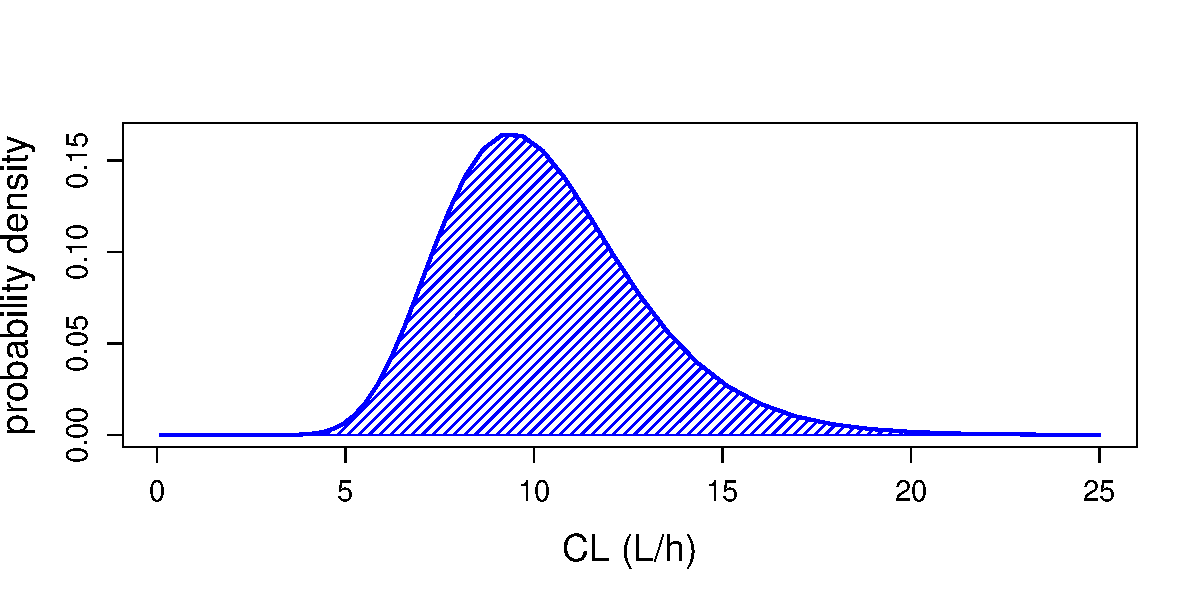
\includegraphics[width=4.5in]{graphics/clDensity001.pdf}}}
\only<2>{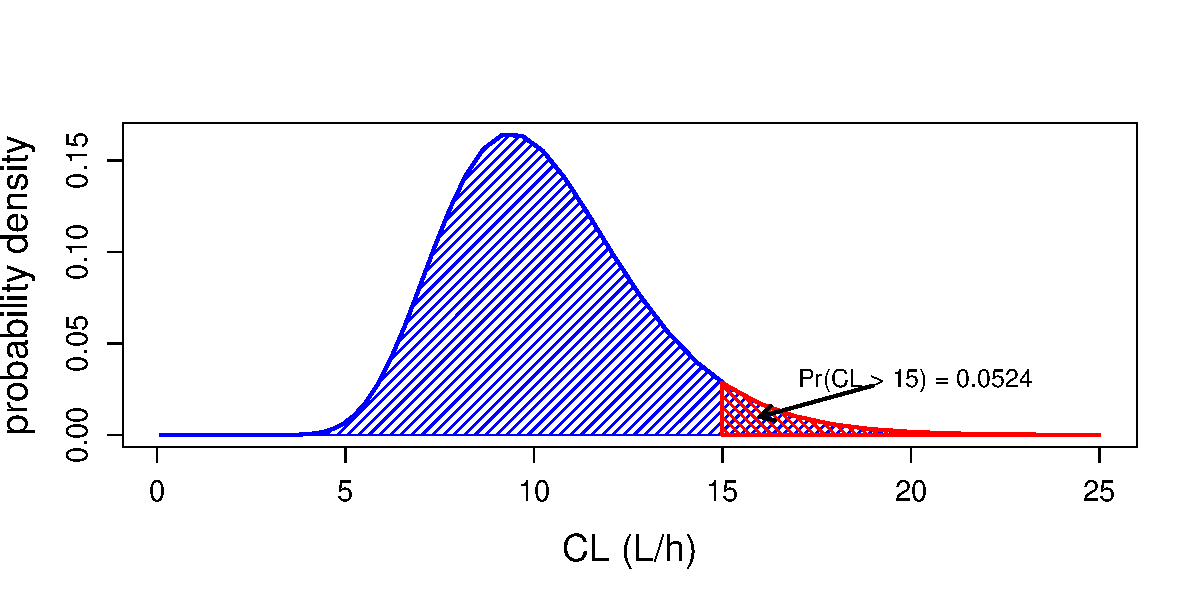
\includegraphics[width=4.5in]{graphics/clDensity002.pdf}}

\end{frame}

\subsection{Bayesian approach to statistical inference}

\begin{frame}{Bayesian approach to statistical inference}

\begin{itemize}
\item Model parameters and predictions are described in terms of probability distributions representing uncertainty.
\item Results reflect the combined evidence of data and prior knowledge or belief.
\item Focuses on estimation and inferences related to probabilities of unknown quantities: parameters, future data, hypotheses.
\item Inferences may be described directly in terms of probabilities, e.g.,
\begin{itemize}
  \item What is the probability that a parameter or a function of parameters is
  within or outside of a specific interval?
  \item What is the lowest dose that will achieve a $\ge$ 80\% probability
    of reaching an efficacy or safety target?
\end{itemize}
\end{itemize}

\end{frame}

%\subsection{Bayesian applications}

\begin{frame}<article>{Bayesian applications}

\begin{block}{Decision analysis}
\begin{itemize}
\item Bayesian principles are well-suited to decision-making
\begin{itemize}
\item  Assess probable outcomes of different decisions via predictive probabilities
\item Choose decision that maximizes average gain (minimizes average loss) 
\end{itemize}
\end{itemize}
\end{block}

\begin{block}{Modeling and simulation}
\begin{itemize}
\item  Bayesian modeling and simulation are practical options for many applications due to advances in hardware, numerical methods and software.
\item Now possible to model complex nonlinear systems (e.g., PK/PD) and processes (e.g., clinical trials).
\end{itemize}
\end{block}

\end{frame}

\subsection{Bayesian inference}

\begin{frame}{Bayesian inference}
\framesubtitle{\large Bayes Rule}

\alert{Bayes Rule} is the basis for inference about model parameters ($\theta$) given data ($y$) and prior knowledge about model parameters ($p\left(\theta\right)$):
\begin{eqnarray*}
p\left(\theta|y\right) &=& \frac{p\left(\theta\right)p\left(y|\theta\right)}{p\left(y\right)}
= \frac{p\left(\theta\right)p\left(y|\theta\right)}{\int{p\left(\theta\right)p\left(y|\theta\right) d\theta}}
\\ 
&\propto& p\left(\theta\right)p\left(y|\theta\right)
\end{eqnarray*}
The $p$'s are probabilities or probability densities of the specified random variables.

\end{frame}

%\note[item]{This slide and the next are the most important w.r.t. understanding the fundamentals of the Bayesian approach. }
%\note[item]{Explain the slides in detail and make sure the particpants understand this is the core of everything we do in the rest of the course. }

\begin{frame}{Bayesian modeling/inference process}

\begin{enumerate}
\item Assess prior distribution $p\left(\theta\right)$
\begin{itemize}
 \item $\theta$ viewed as random variables
\item Subjective
\item Ideally base on all available evidence/knowledge (or belief)
\item Or deliberately select a non-informative prior (e.g., reference, vague or improper prior)
\end{itemize}
\item<2-> Construct a model for the data $p\left(y | \theta\right)$, also known as the likelihood function when viewed as a function of $\theta$.
\note<2>[item]{$p\left(y | \theta\right)$ is not new to you. It is exactly the same as the model you specify when using ML methods.}
\item<3-> Calculate posterior distribution $p\left(\theta | y\right)$.
\begin{itemize}
\item Use for inferences regarding parameter values
\end{itemize}
\item<4-> Calculate posterior predictive distribution $p\left(y_\text{new} | y\right)$.
\begin{itemize}
\item  Use for inferences regarding future observations
\end{itemize}
\end{enumerate}
\onslide<4->{$$p\left(y_{new}|y\right) = \int{p\left(y_{new}|\theta\right)p\left(\theta|y\right) d\theta}$$}

\end{frame}

\begin{frame}{A simple one parameter example}

Estimating the mean of a normal distribution with a known variance where the prior is also normal:
\begin{footnotesize}
\begin{eqnarray*}
\theta &\sim& N\left(\mu_0,\tau_0\right) \ \ \ \ \ \ \ \ \ \ \ \ \ \ \ 
y|\theta \sim N\left(\theta,\sigma\right) \\
\onslide<2->{
p\left(\theta|y\right) &\propto& p\left(\theta\right)p\left(y|\theta\right) = p\left(\theta\right)\prod_{i=1}^n p\left(y_i|\theta\right) \\}
\onslide<3->{
&\propto& \exp\left(-\frac{1}{2\tau_0^2}\left(\theta-\mu_0\right)^2\right)\prod_{i=1}^n \exp\left(-\frac{1}{2\sigma^2}\left(y_i-\theta\right)^2\right) \\
&\propto& \exp\left(-\frac{1}{2}\left[\frac{1}{\tau_0^2}\left(\theta-\mu_0\right)^2 + \frac{1}{\sigma^2}\sum_{i=1}^n \left(y_i-\theta\right)^2\right]\right) \\}
\onslide<4->{
&\Downarrow& \\
\theta|y &\sim& N\left(\mu_n,\tau_n\right) \\
\mu_n &=& \frac{\frac{1}{\tau_0^2}\mu_0 + \frac{n}{\sigma^2}\overline{y}}{\frac{1}{\tau_0^2} + \frac{n}{\sigma^2}} \;\;{\rm and}\;\;
\tau_n^2 = \frac{1}{\frac{1}{\tau_0^2} + \frac{n}{\sigma^2}}}
\end{eqnarray*}
\end{footnotesize}

\end{frame}

\begin{frame}{A simple one parameter example}

\vspace{-0.1in}
\begin{footnotesize}
\begin{itemize}
\item Posterior mean is a weighted average of prior mean ($\mu_0$) and the sample mean ($\overline{y}$).
\item Posterior precision $\left(\frac{1}{\tau_n^2}\right)$ is a sum of the prior precision $\left(\frac{1}{\tau_0^2}\right)$ and the data precision $\left(\frac{n}{\sigma^2}\right)$.
\item The prior can also be interpreted in terms of equivalent number of data points, i.e., $n_0 = \frac{\sigma^2}{\tau_0^2}$.
\end{itemize}
\end{footnotesize}
\vspace{-0.5in}
\only<1>{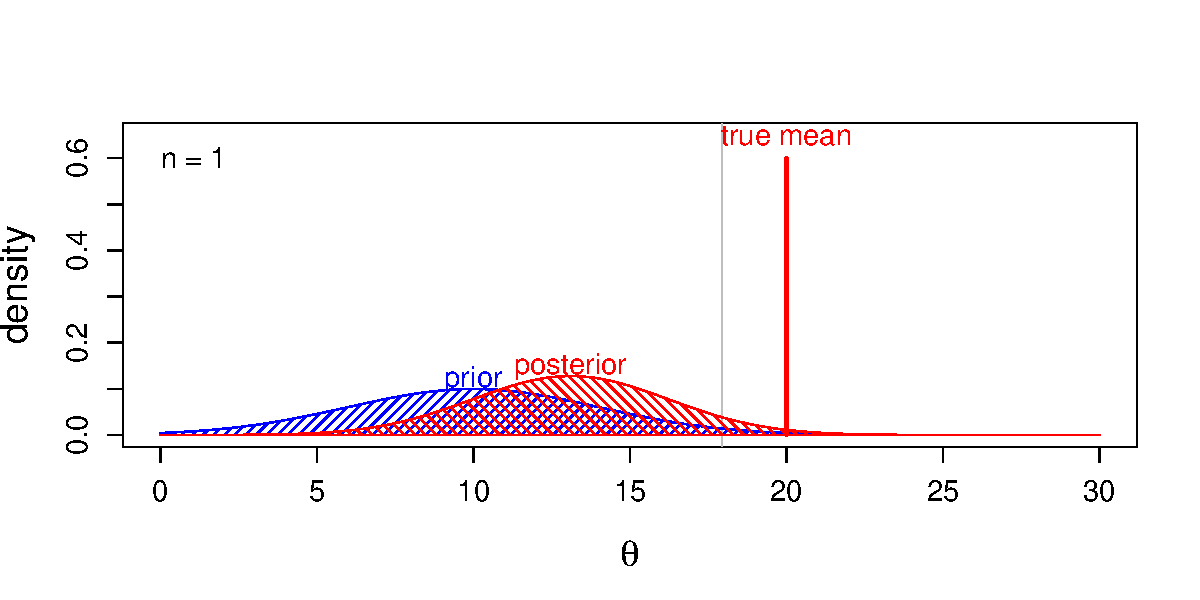
\includegraphics[width=5in]{graphics/updateExample001.pdf}}
\mode<beamer>{\only<2>{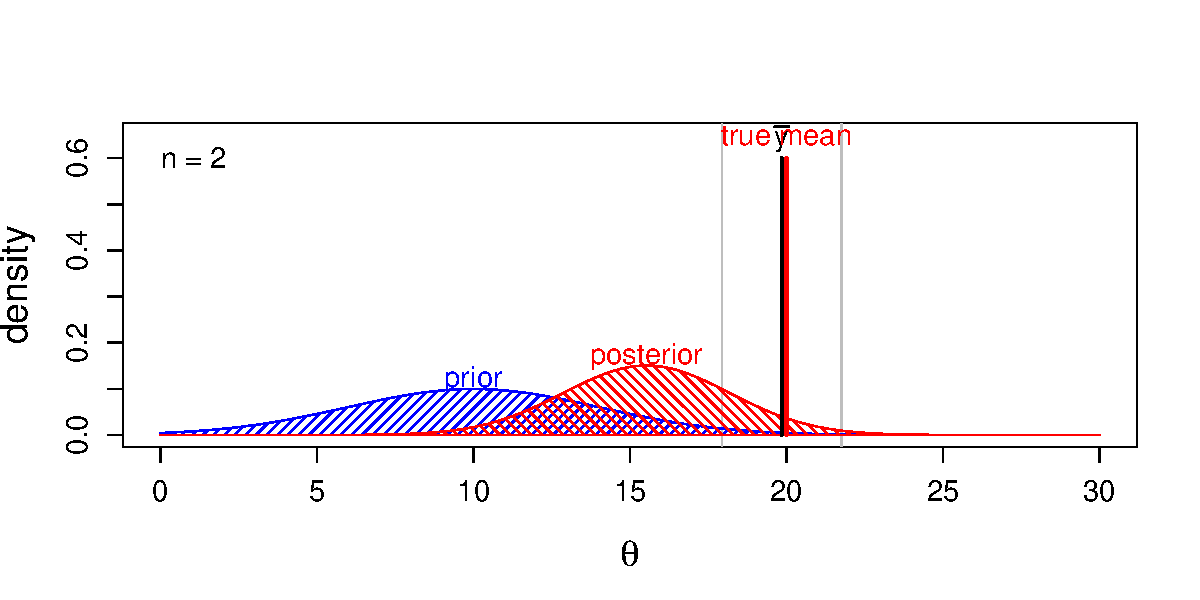
\includegraphics[width=5in]{graphics/updateExample002.pdf}}}
\mode<beamer>{\only<3>{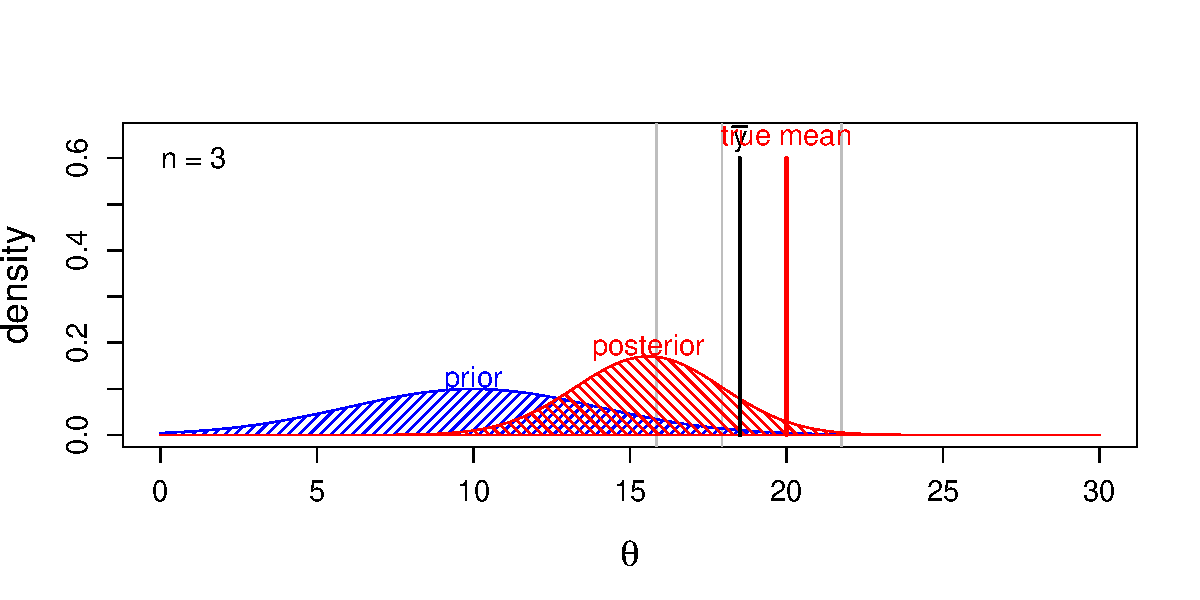
\includegraphics[width=5in]{graphics/updateExample003.pdf}}}
\mode<beamer>{\only<4>{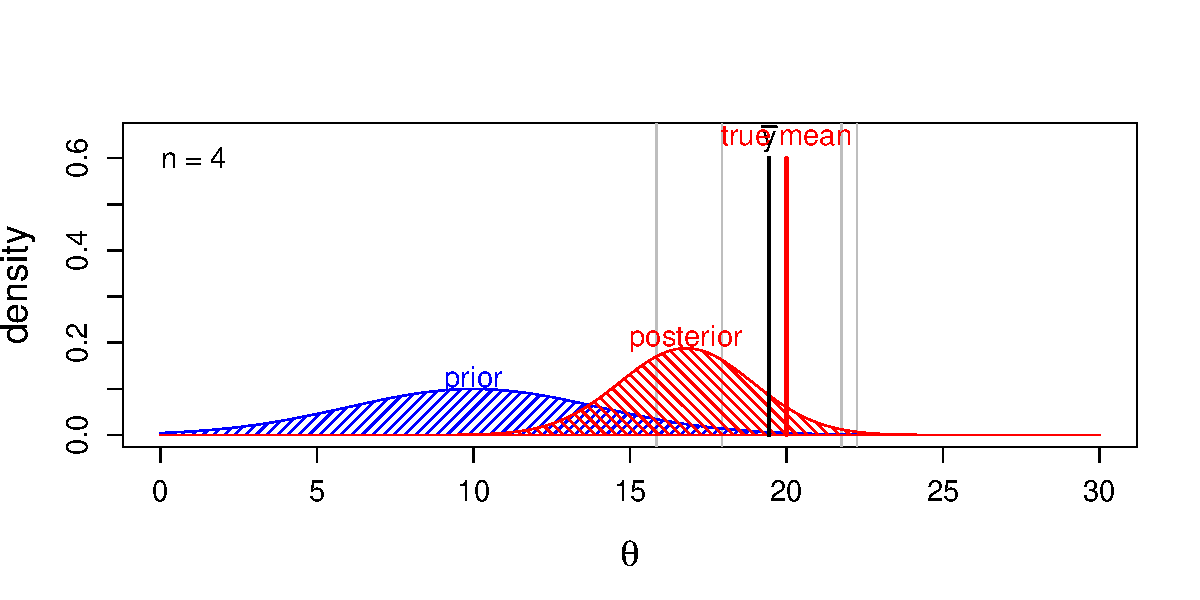
\includegraphics[width=5in]{graphics/updateExample004.pdf}}}
\mode<beamer>{\only<5>{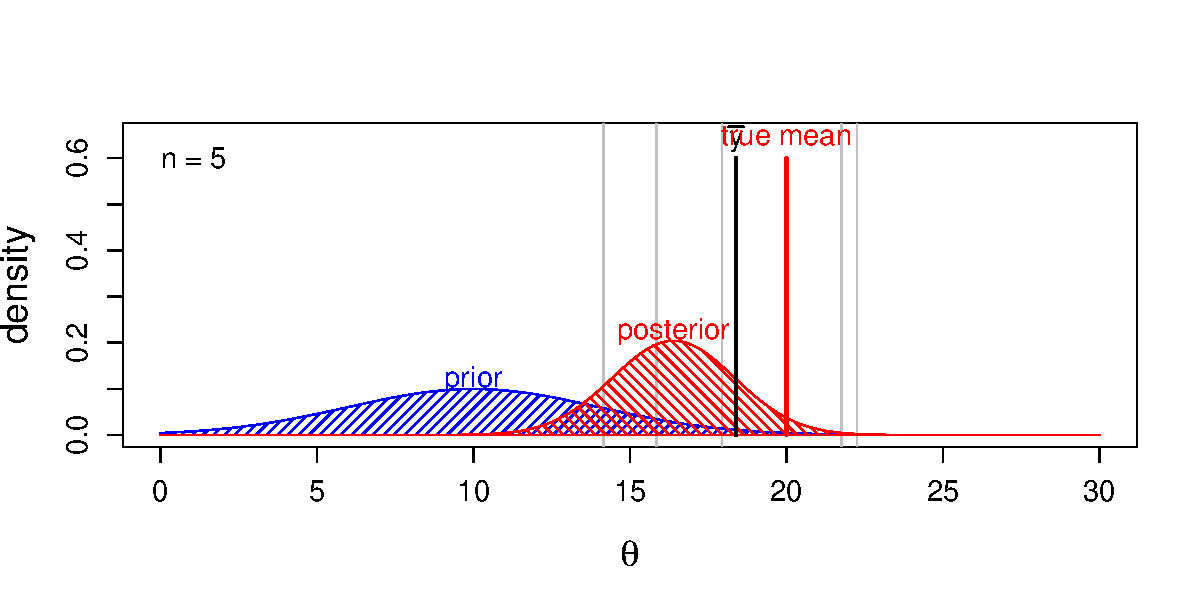
\includegraphics[width=5in]{graphics/updateExample005.pdf}}}
\mode<beamer>{\only<6>{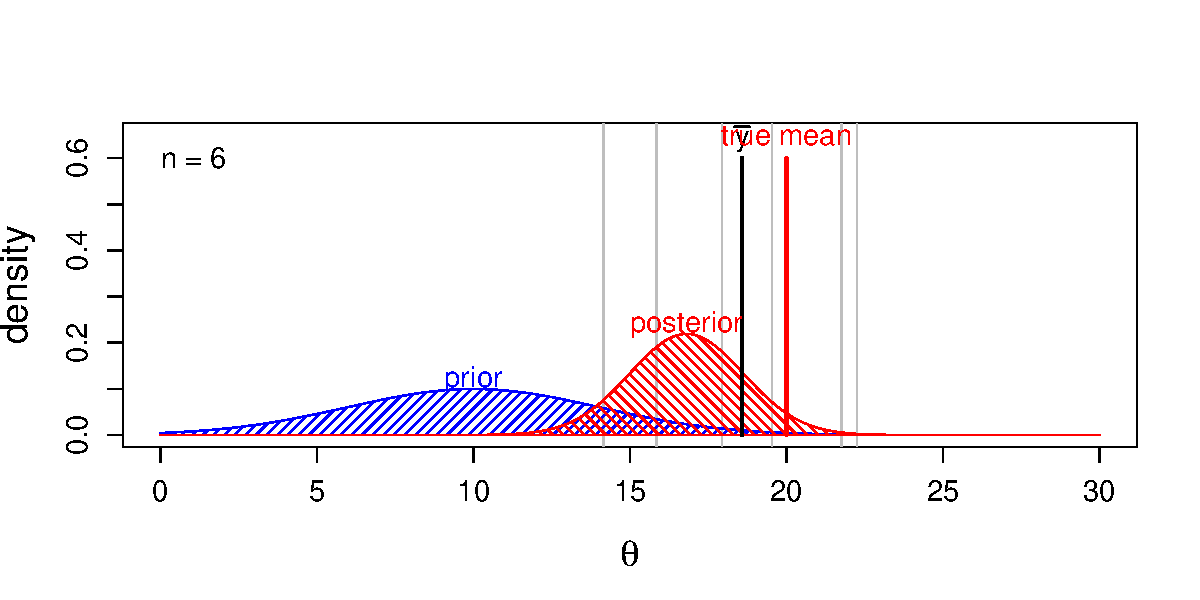
\includegraphics[width=5in]{graphics/updateExample006.pdf}}}
\mode<beamer>{\only<7>{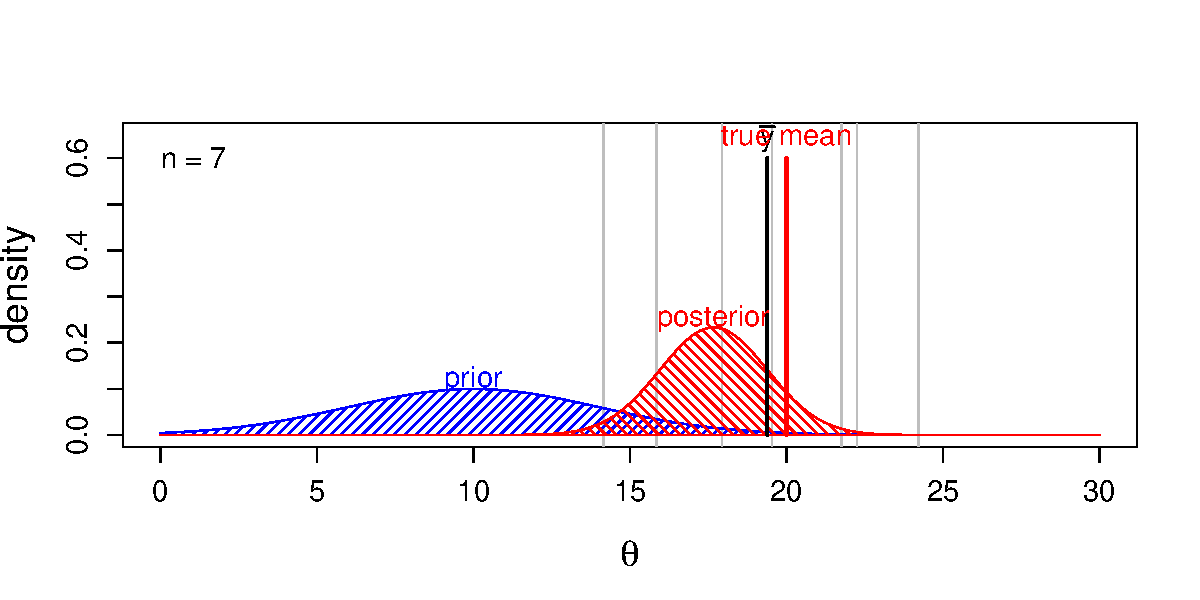
\includegraphics[width=5in]{graphics/updateExample007.pdf}}}
\mode<beamer>{\only<8>{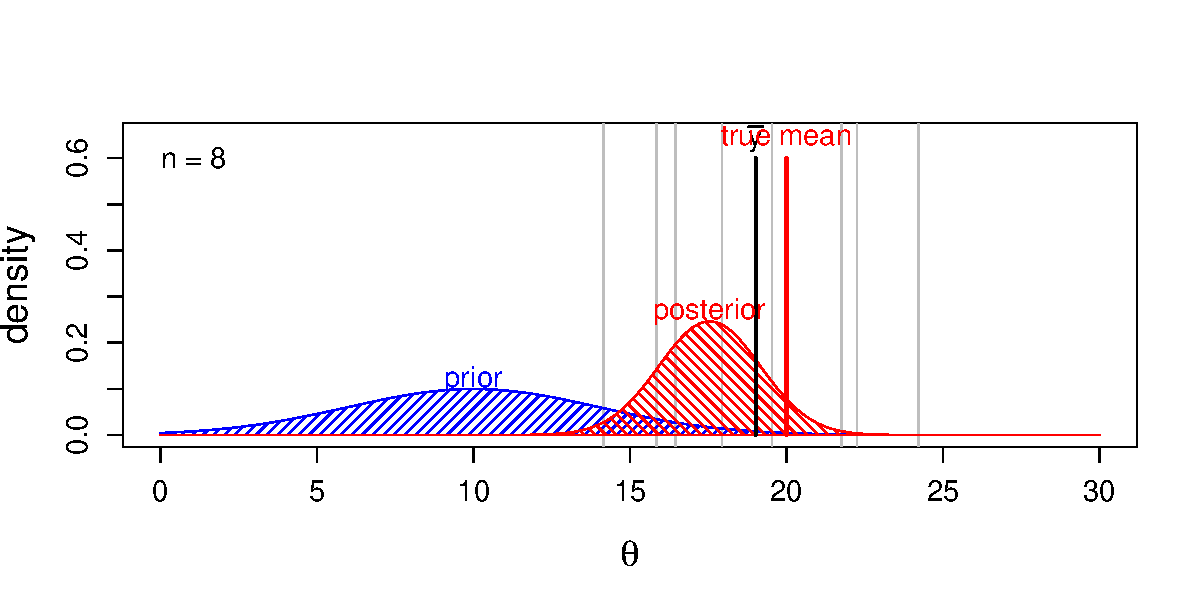
\includegraphics[width=5in]{graphics/updateExample008.pdf}}}
\mode<beamer>{\only<9>{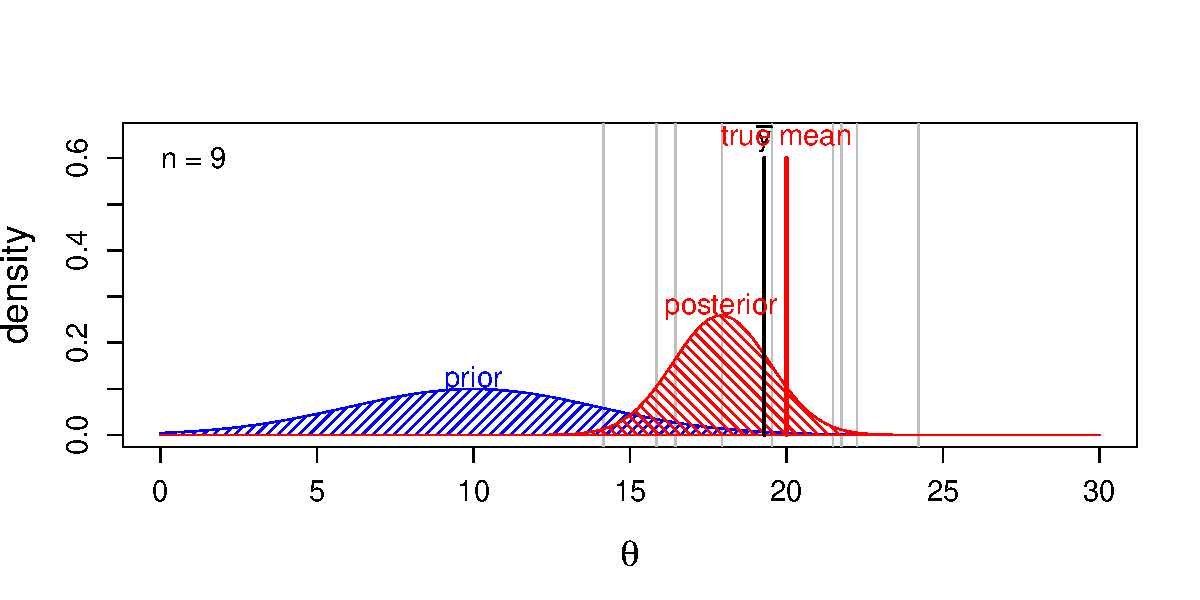
\includegraphics[width=5in]{graphics/updateExample009.pdf}}}
\mode<beamer>{\only<10>{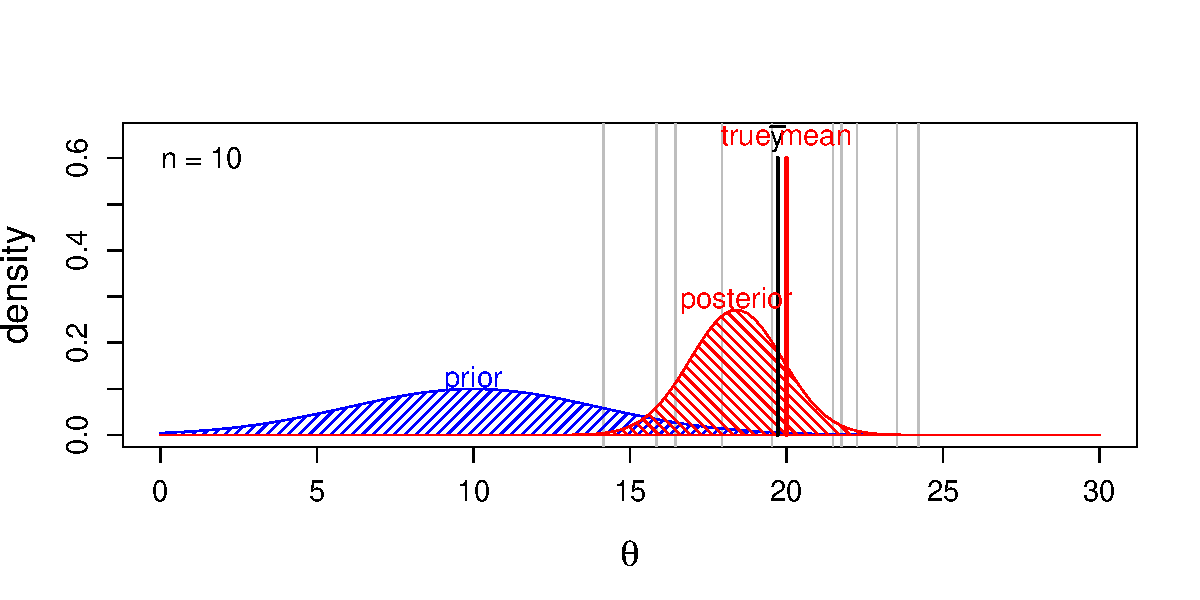
\includegraphics[width=5in]{graphics/updateExample010.pdf}}}
\mode<beamer>{\only<11>{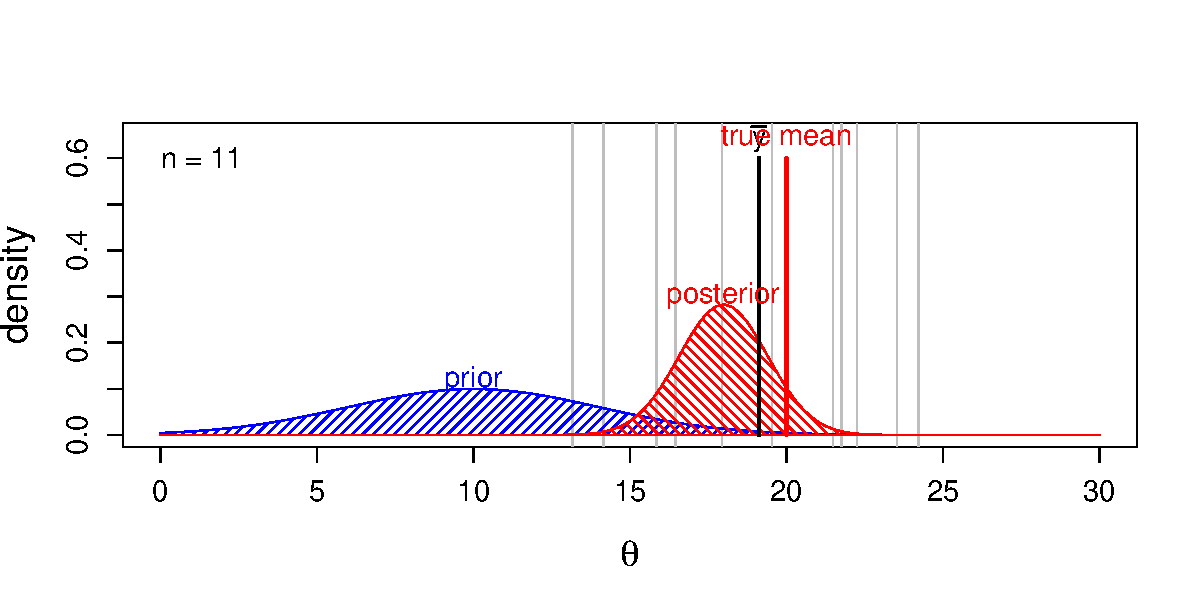
\includegraphics[width=5in]{graphics/updateExample011.pdf}}}
\mode<beamer>{\only<12>{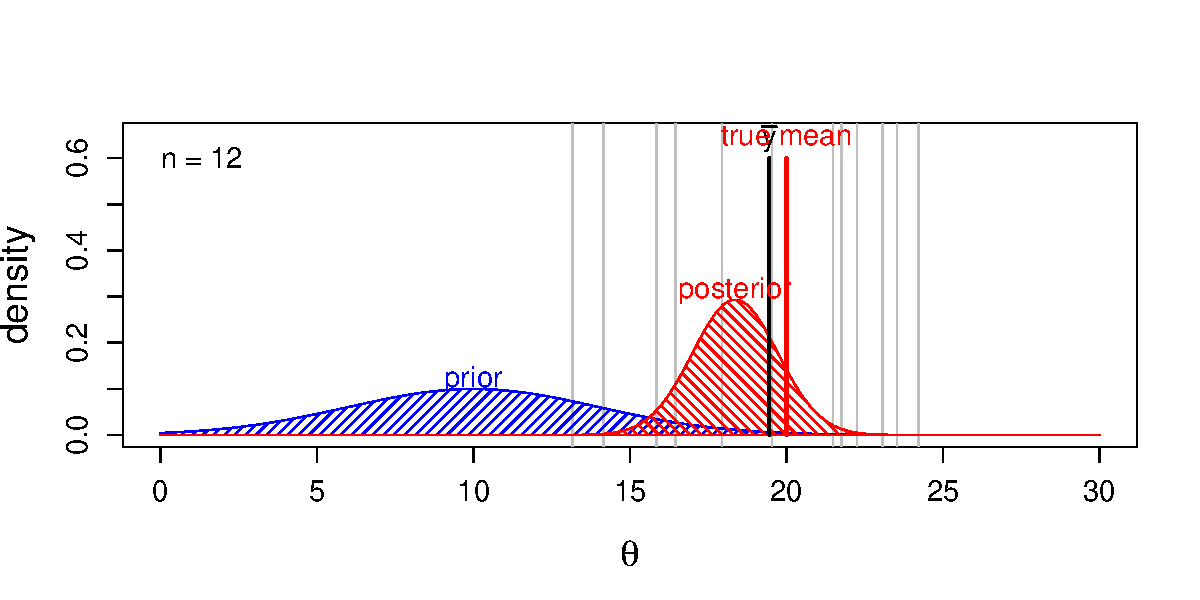
\includegraphics[width=5in]{graphics/updateExample012.pdf}}}
\mode<beamer>{\only<13>{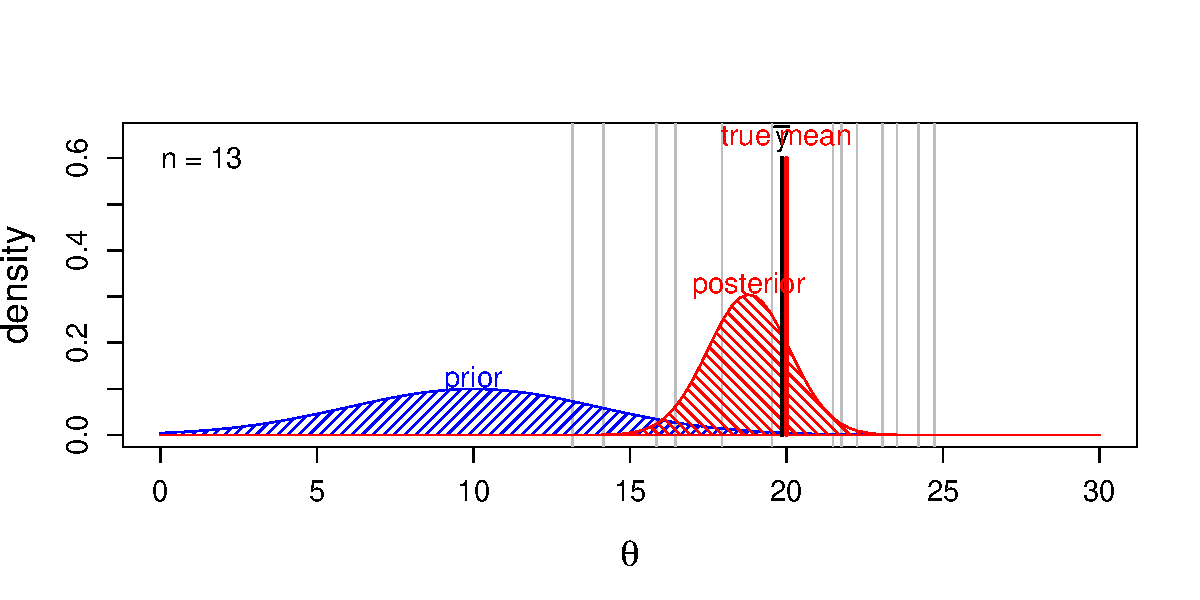
\includegraphics[width=5in]{graphics/updateExample013.pdf}}}
\mode<beamer>{\only<14>{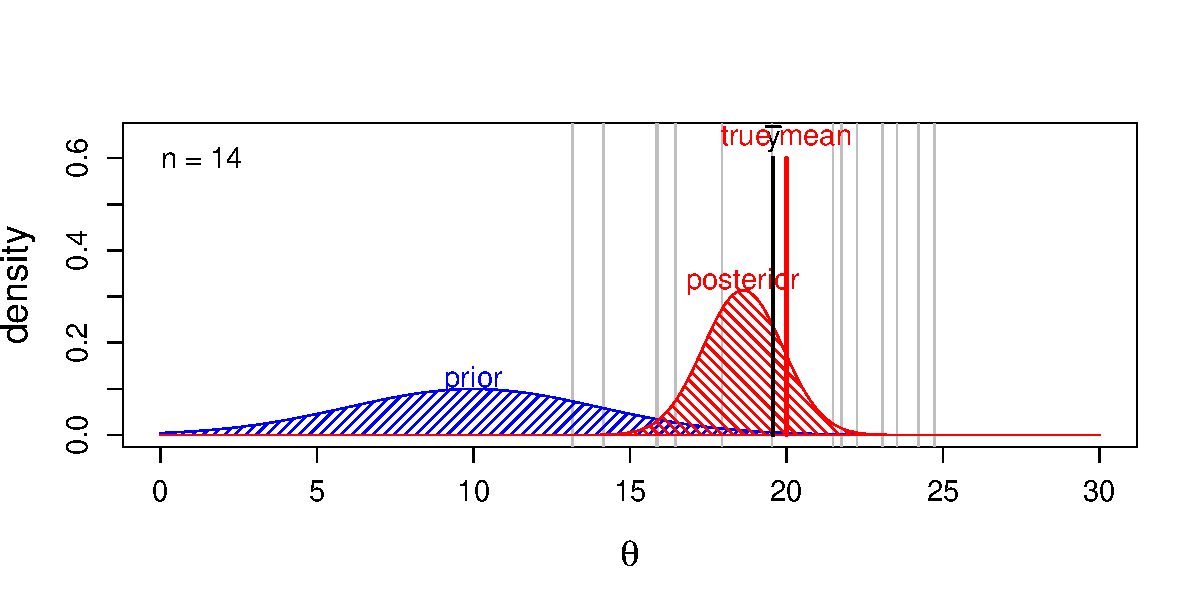
\includegraphics[width=5in]{graphics/updateExample014.pdf}}}
\mode<beamer>{\only<15>{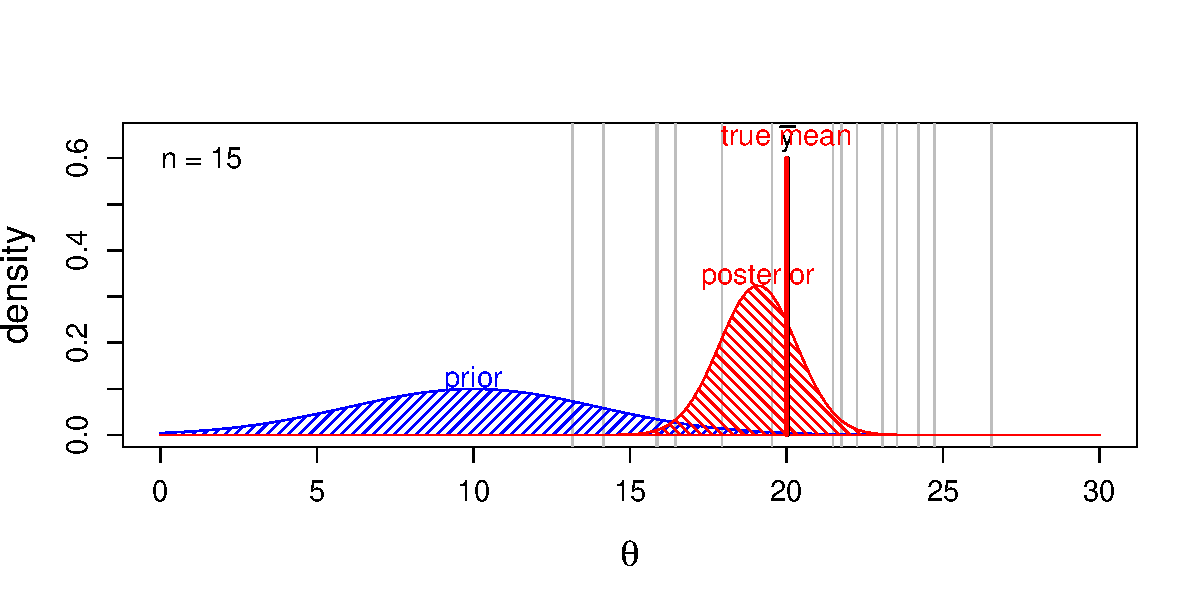
\includegraphics[width=5in]{graphics/updateExample015.pdf}}}
\mode<beamer>{\only<16>{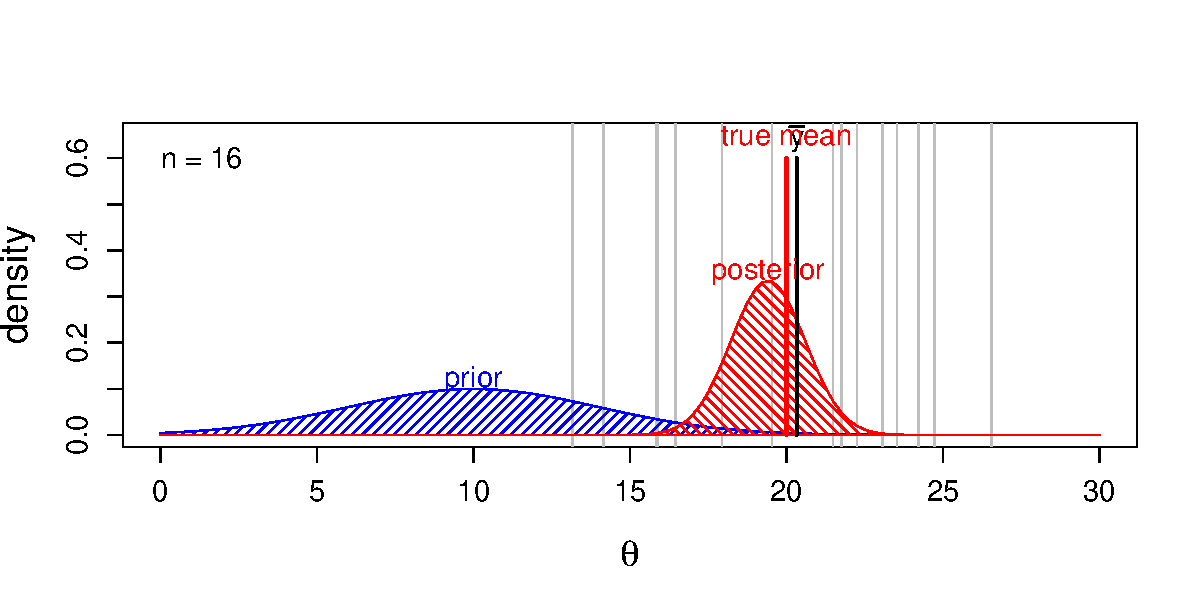
\includegraphics[width=5in]{graphics/updateExample016.pdf}}}
\mode<beamer>{\only<17>{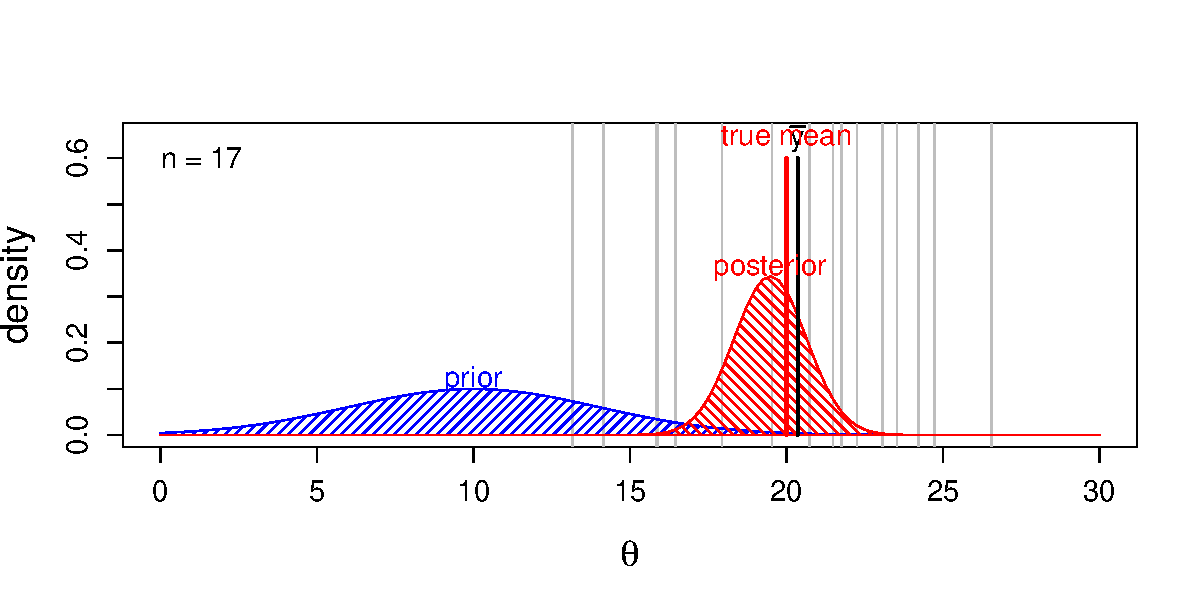
\includegraphics[width=5in]{graphics/updateExample017.pdf}}}
\mode<beamer>{\only<18>{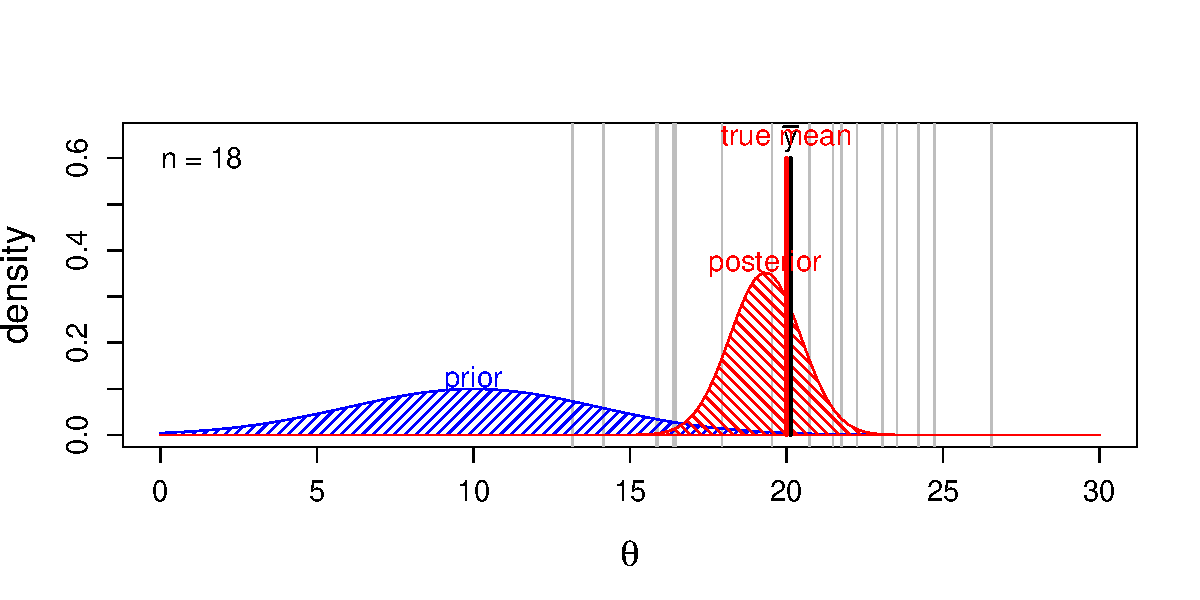
\includegraphics[width=5in]{graphics/updateExample018.pdf}}}
\mode<beamer>{\only<19>{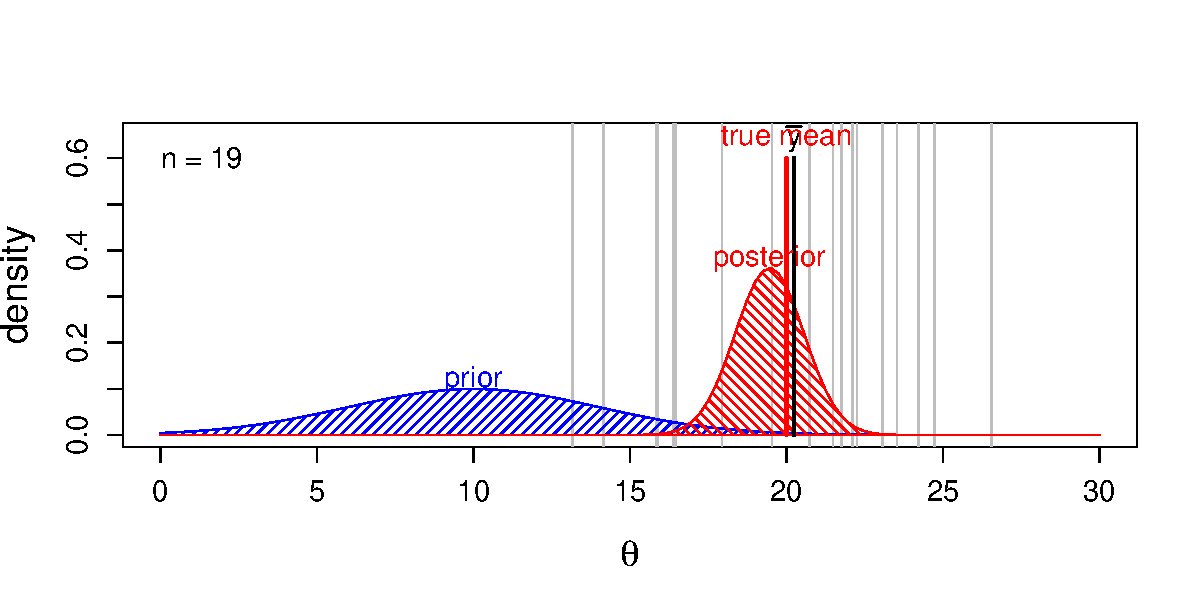
\includegraphics[width=5in]{graphics/updateExample019.pdf}}}
\mode<beamer>{\only<20>{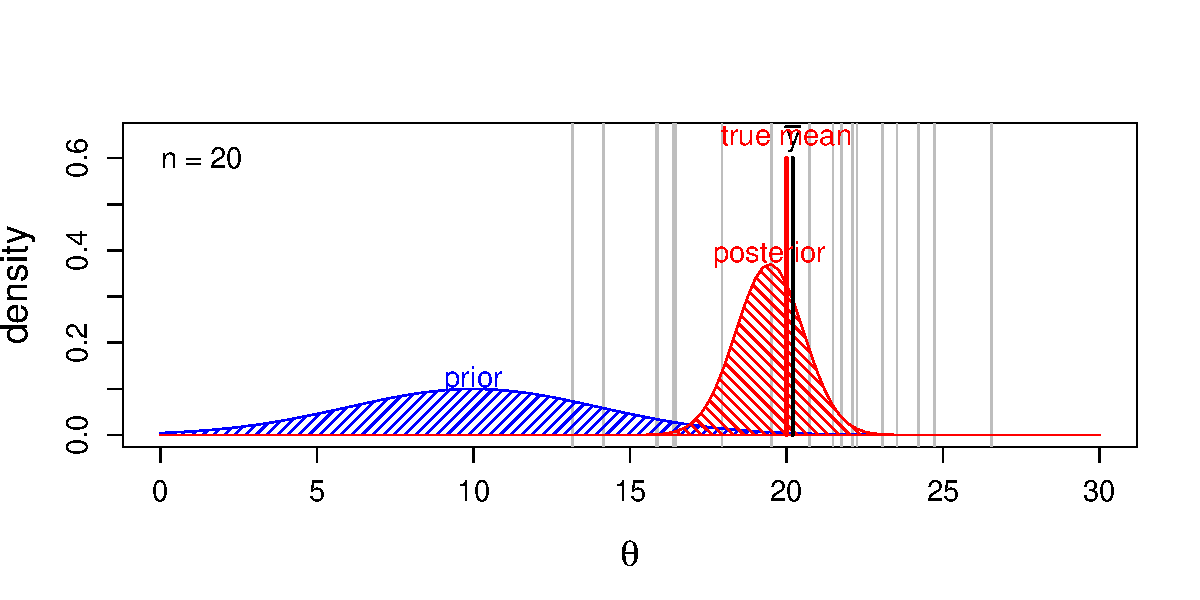
\includegraphics[width=5in]{graphics/updateExample020.pdf}}}
\mode<beamer>{\only<21>{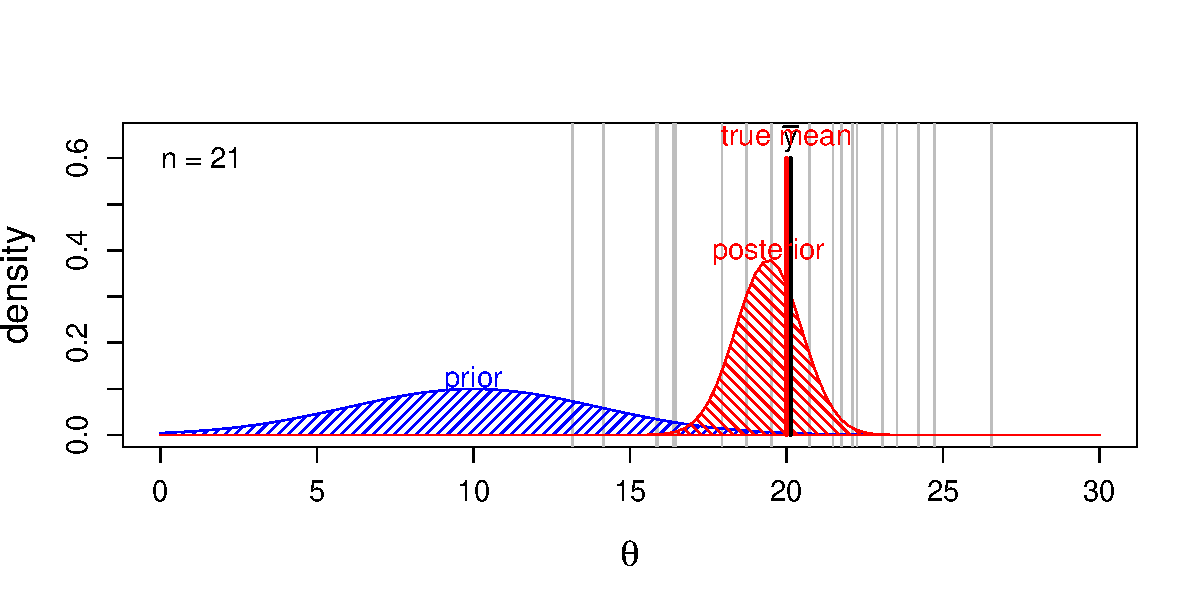
\includegraphics[width=5in]{graphics/updateExample021.pdf}}}
\mode<beamer>{\only<22>{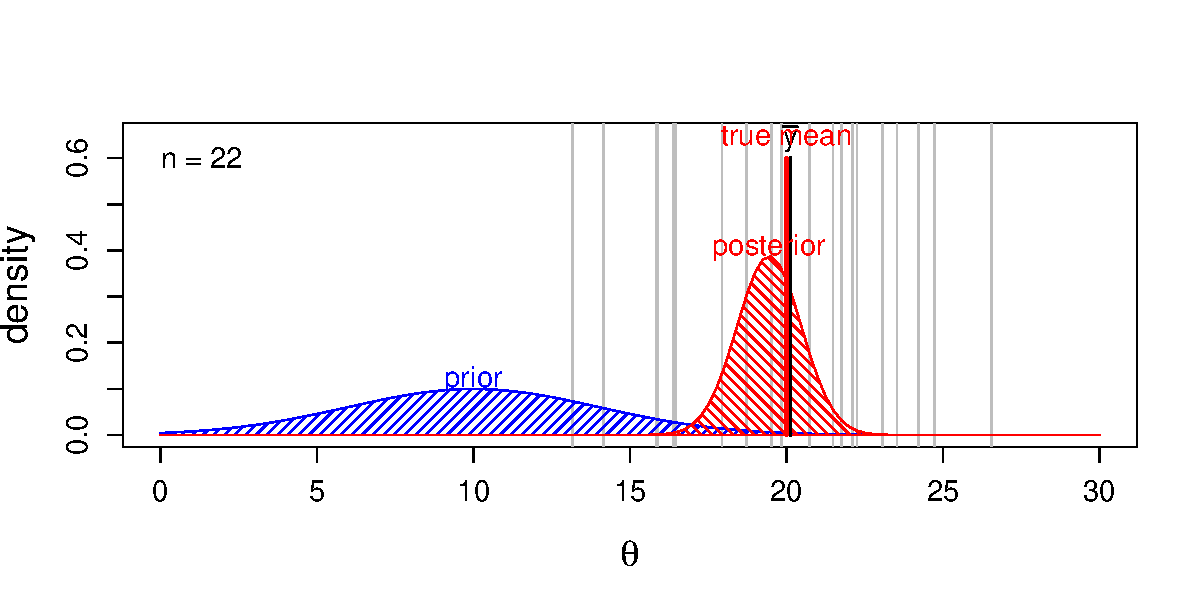
\includegraphics[width=5in]{graphics/updateExample022.pdf}}}
\mode<beamer>{\only<23>{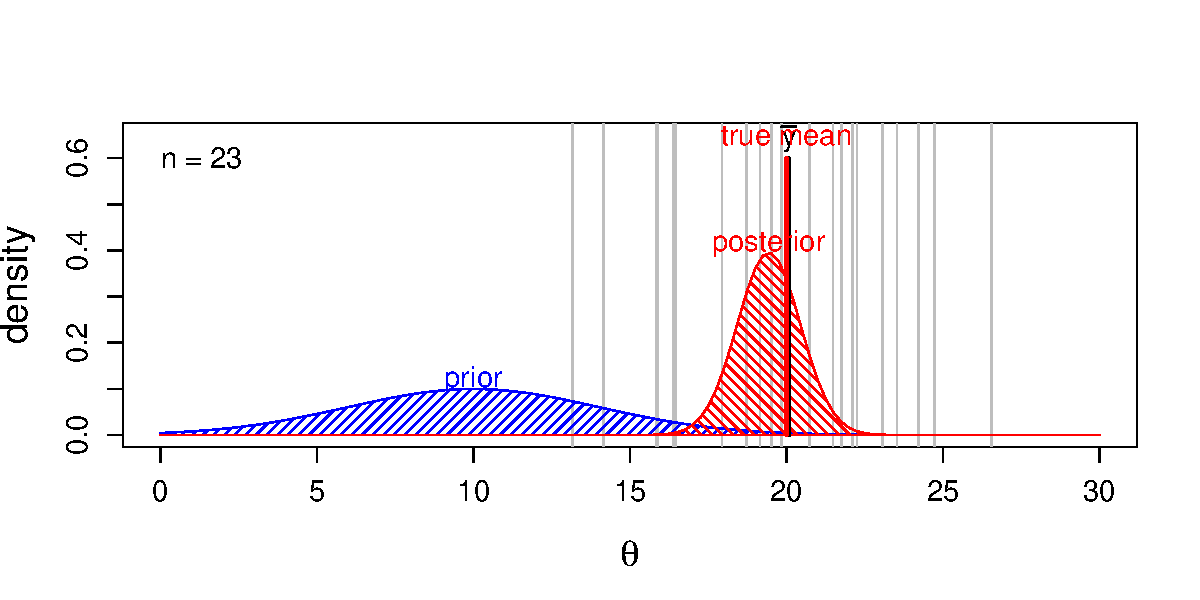
\includegraphics[width=5in]{graphics/updateExample023.pdf}}}
\mode<beamer>{\only<24>{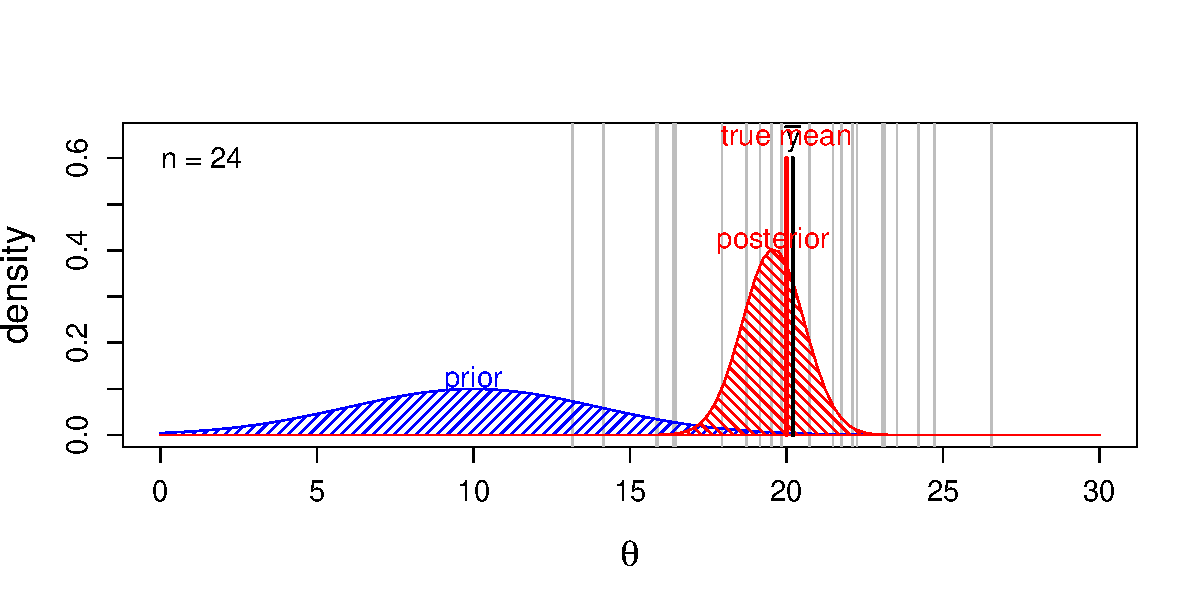
\includegraphics[width=5in]{graphics/updateExample024.pdf}}}
\mode<beamer>{\only<25>{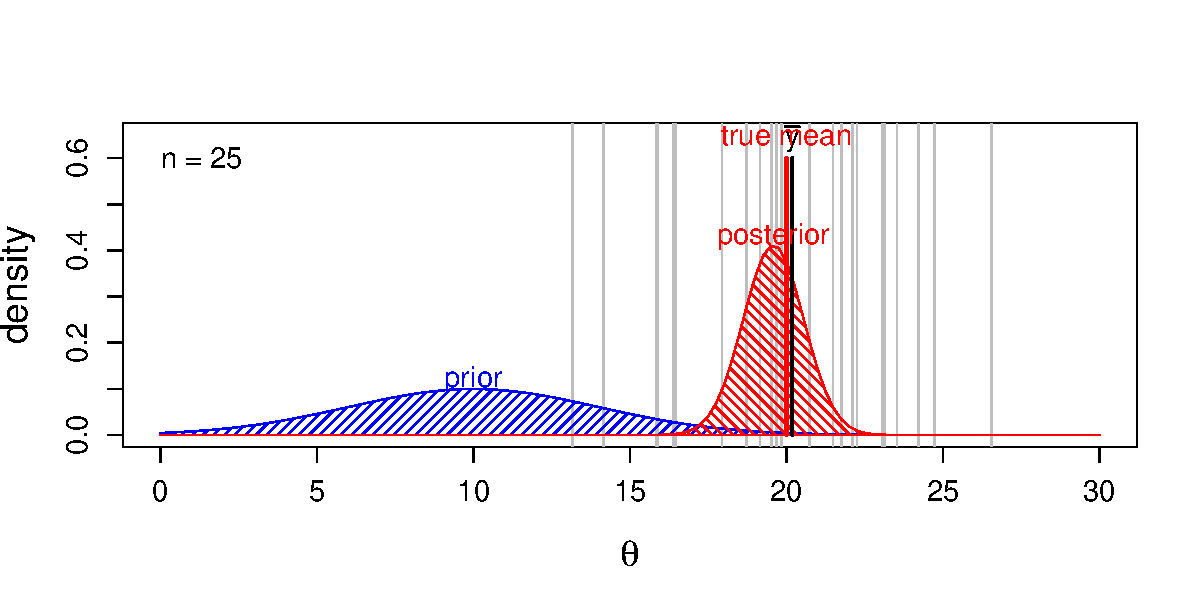
\includegraphics[width=5in]{graphics/updateExample025.pdf}}}
\mode<beamer>{\only<26>{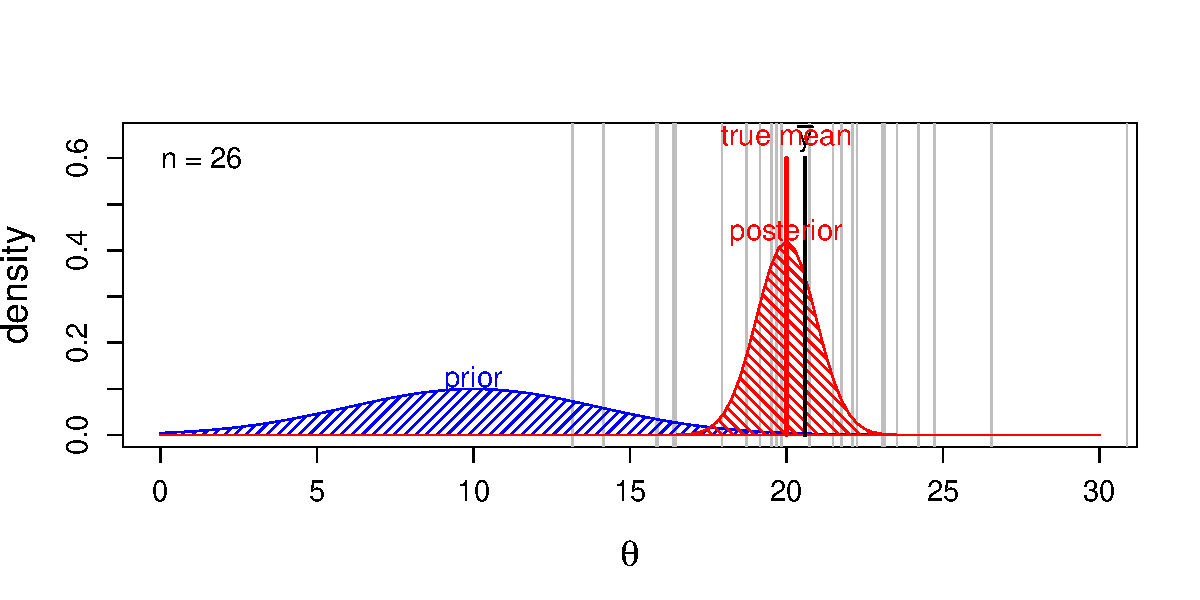
\includegraphics[width=5in]{graphics/updateExample026.pdf}}}
\mode<beamer>{\only<27>{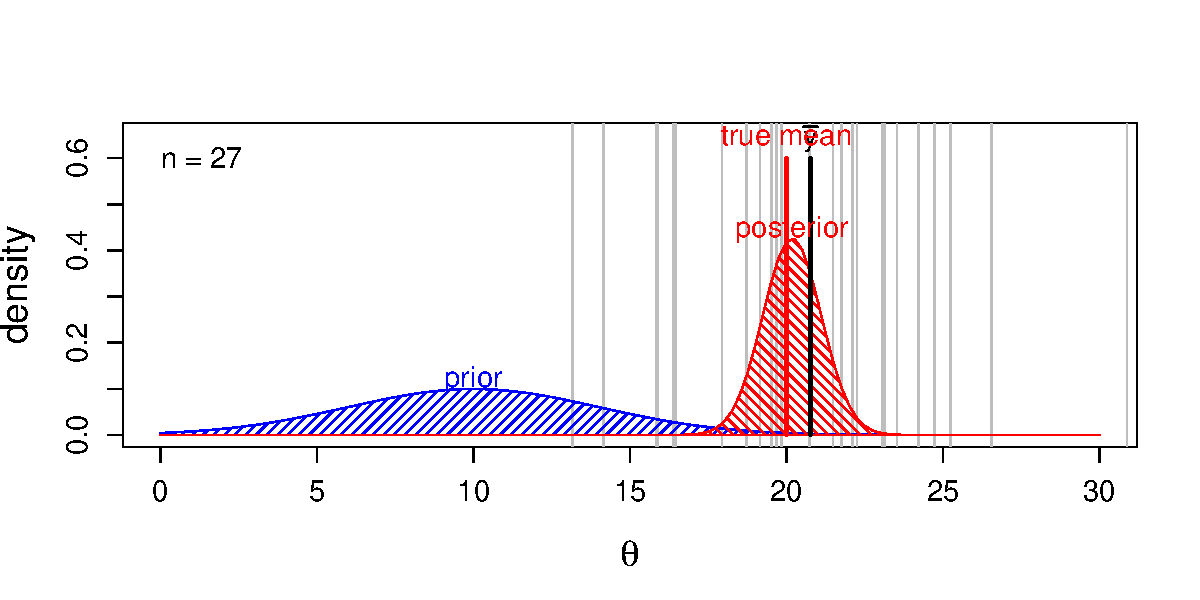
\includegraphics[width=5in]{graphics/updateExample027.pdf}}}
\mode<beamer>{\only<28>{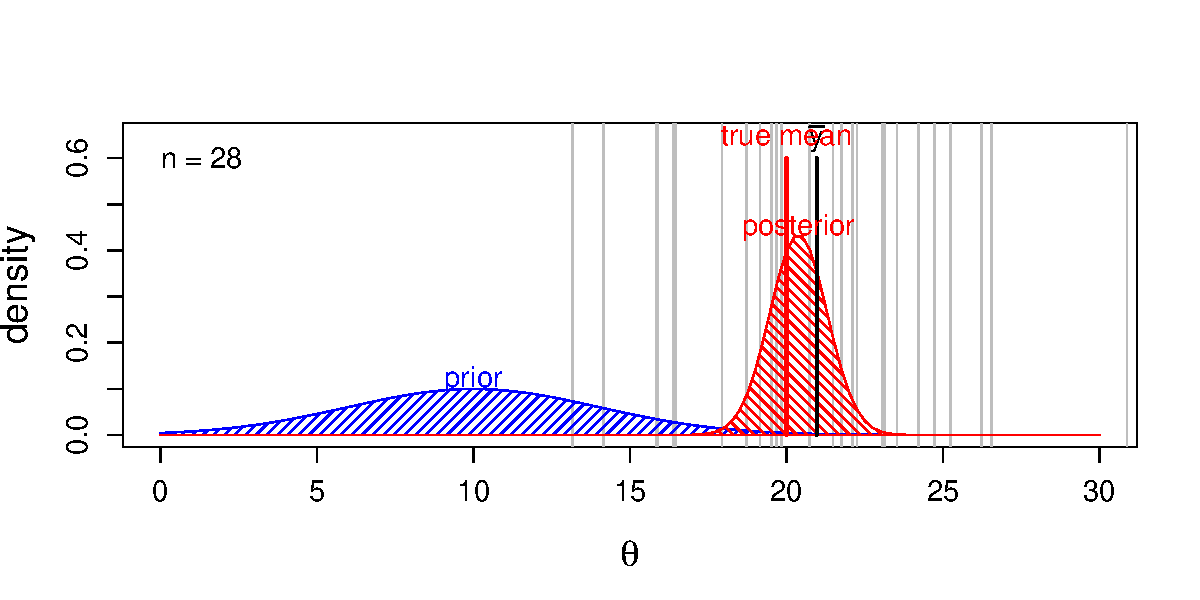
\includegraphics[width=5in]{graphics/updateExample028.pdf}}}
\mode<beamer>{\only<29>{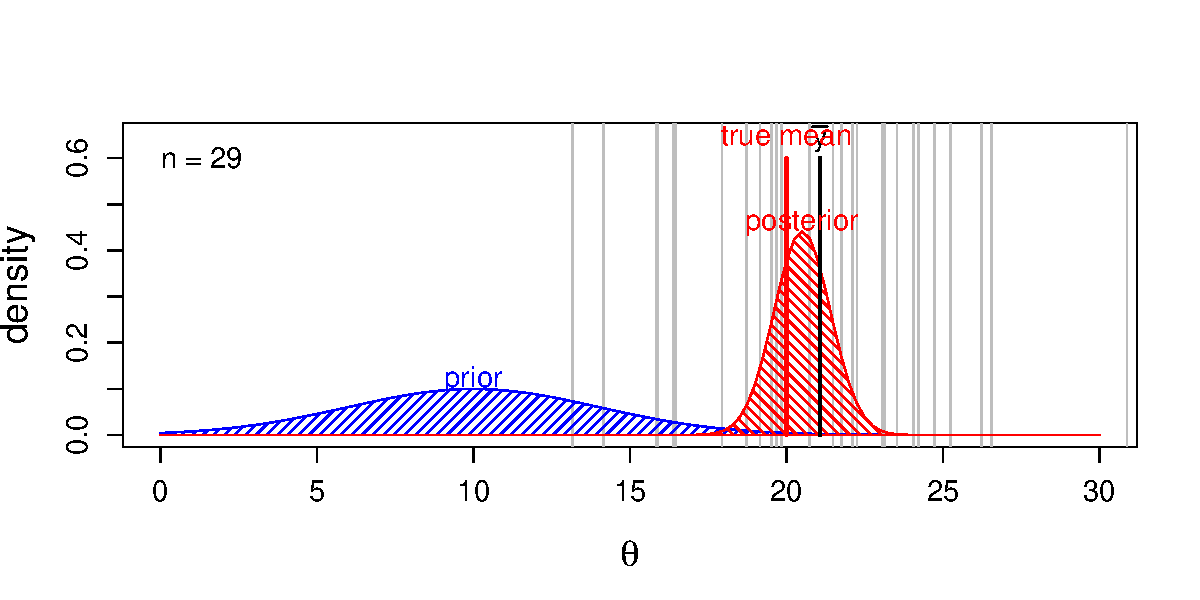
\includegraphics[width=5in]{graphics/updateExample029.pdf}}}
\mode<beamer>{\only<30>{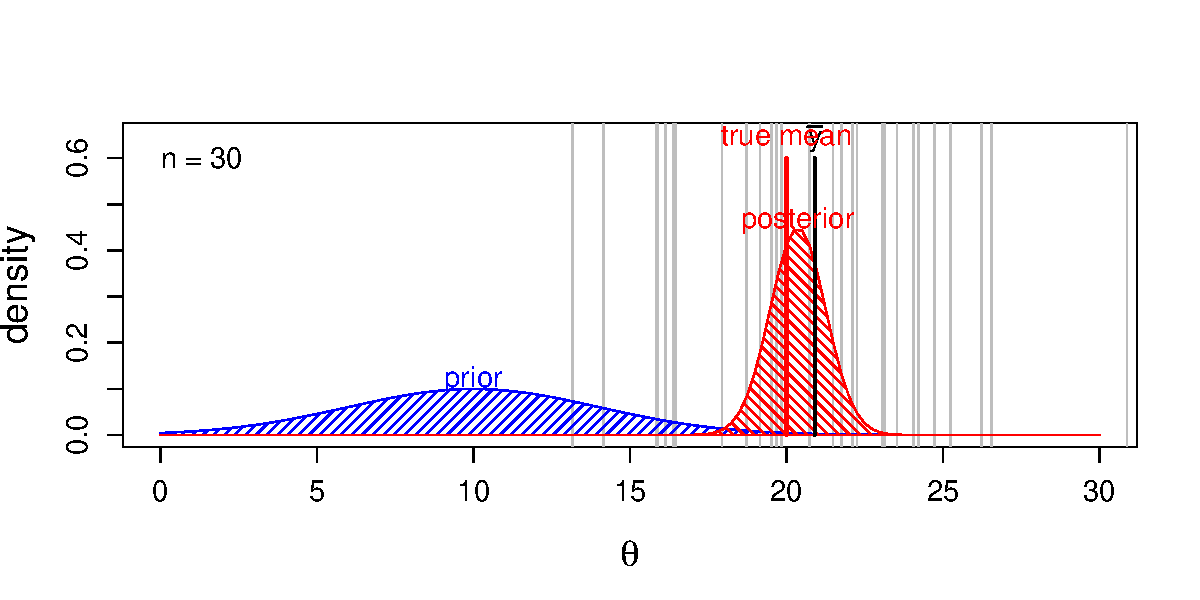
\includegraphics[width=5in]{graphics/updateExample030.pdf}}}
\mode<beamer>{\only<31>{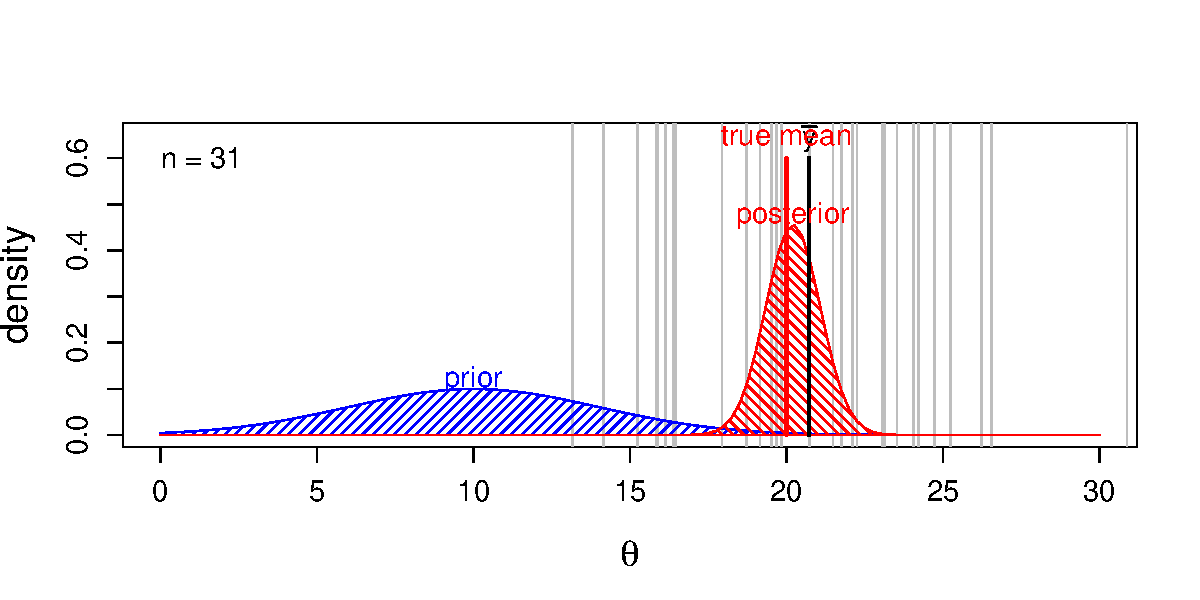
\includegraphics[width=5in]{graphics/updateExample031.pdf}}}
\mode<beamer>{\only<32>{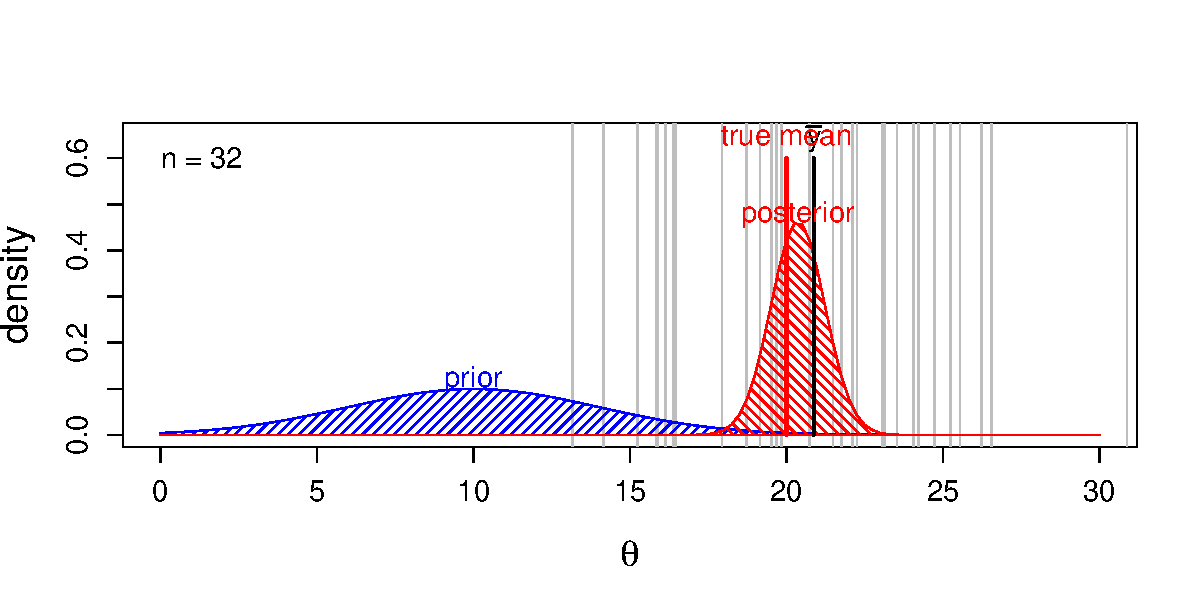
\includegraphics[width=5in]{graphics/updateExample032.pdf}}}
\mode<beamer>{\only<33>{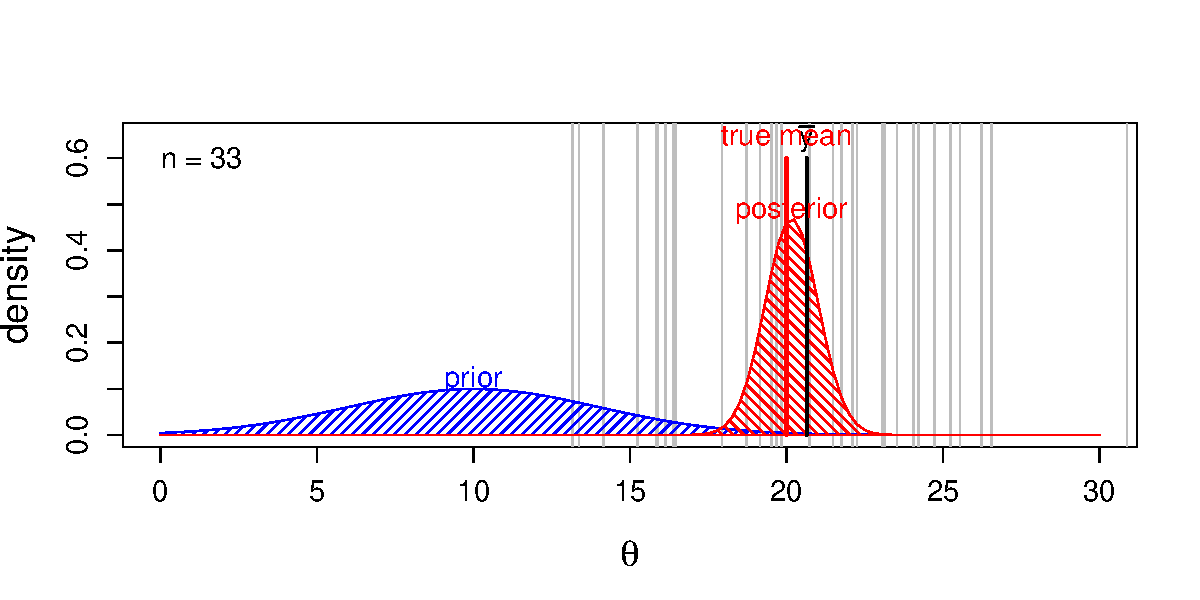
\includegraphics[width=5in]{graphics/updateExample033.pdf}}}
\mode<beamer>{\only<34>{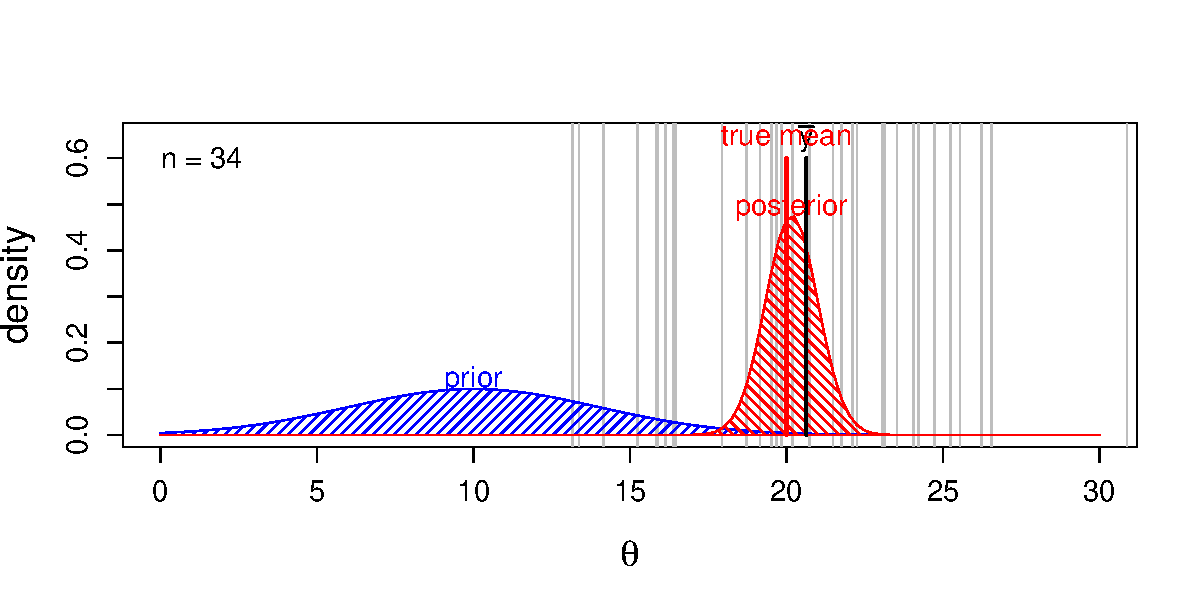
\includegraphics[width=5in]{graphics/updateExample034.pdf}}}
\mode<beamer>{\only<35>{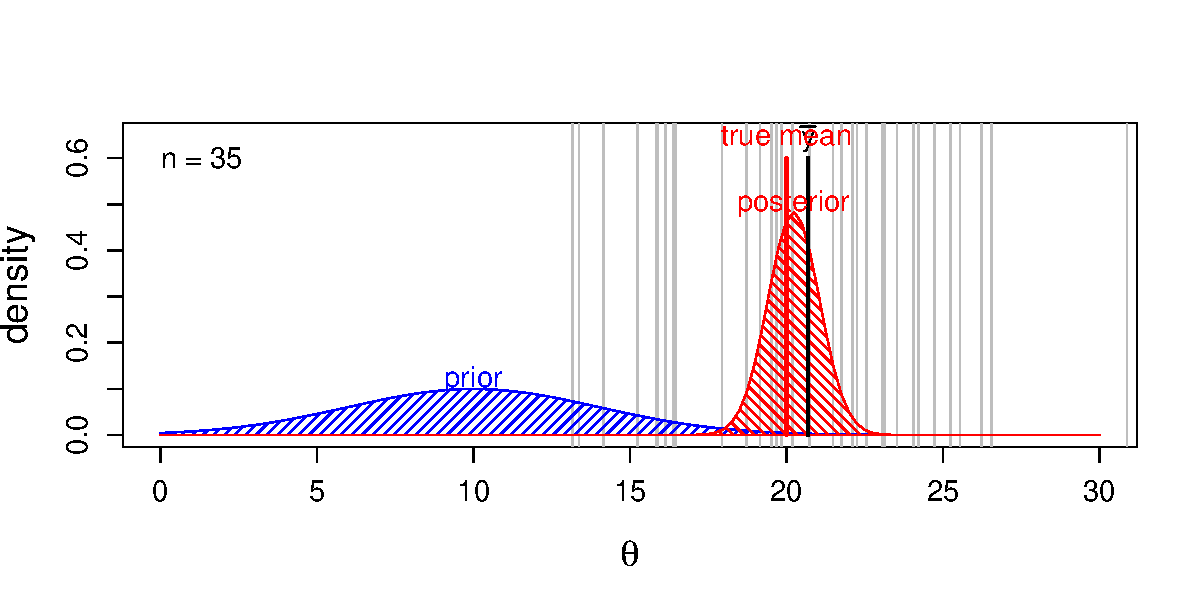
\includegraphics[width=5in]{graphics/updateExample035.pdf}}}
\mode<beamer>{\only<36>{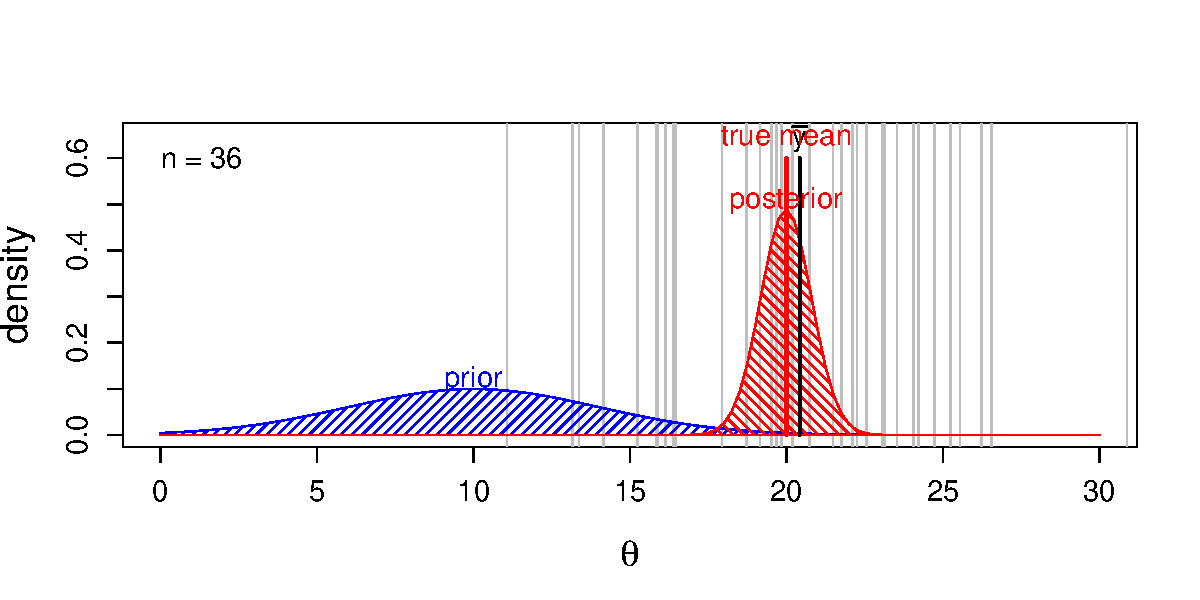
\includegraphics[width=5in]{graphics/updateExample036.pdf}}}
\mode<beamer>{\only<37>{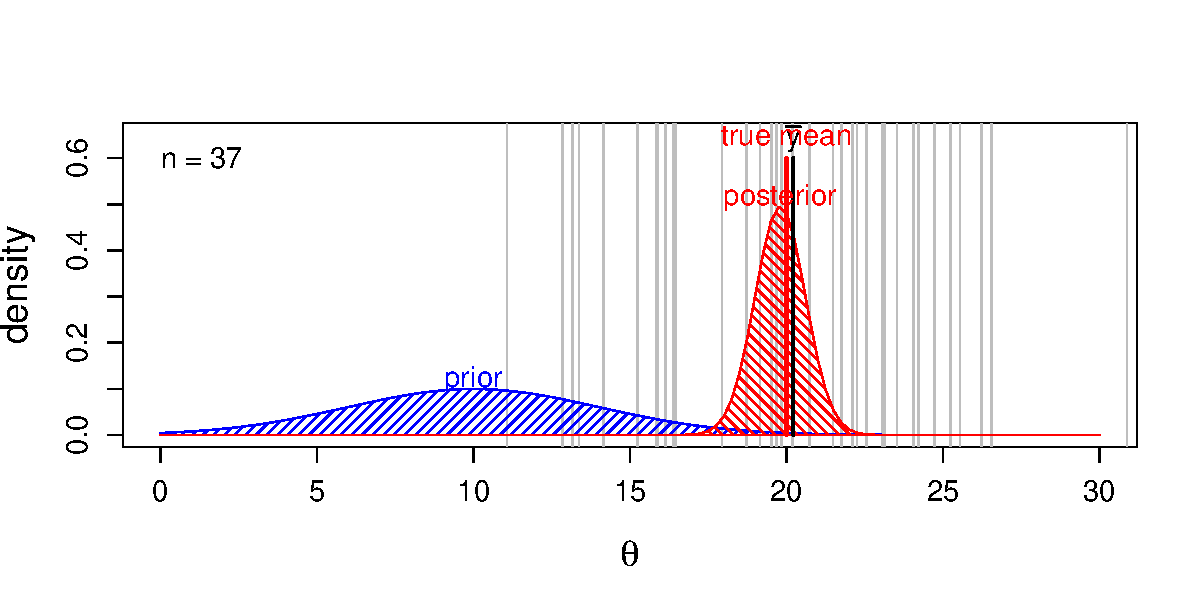
\includegraphics[width=5in]{graphics/updateExample037.pdf}}}
\mode<beamer>{\only<38>{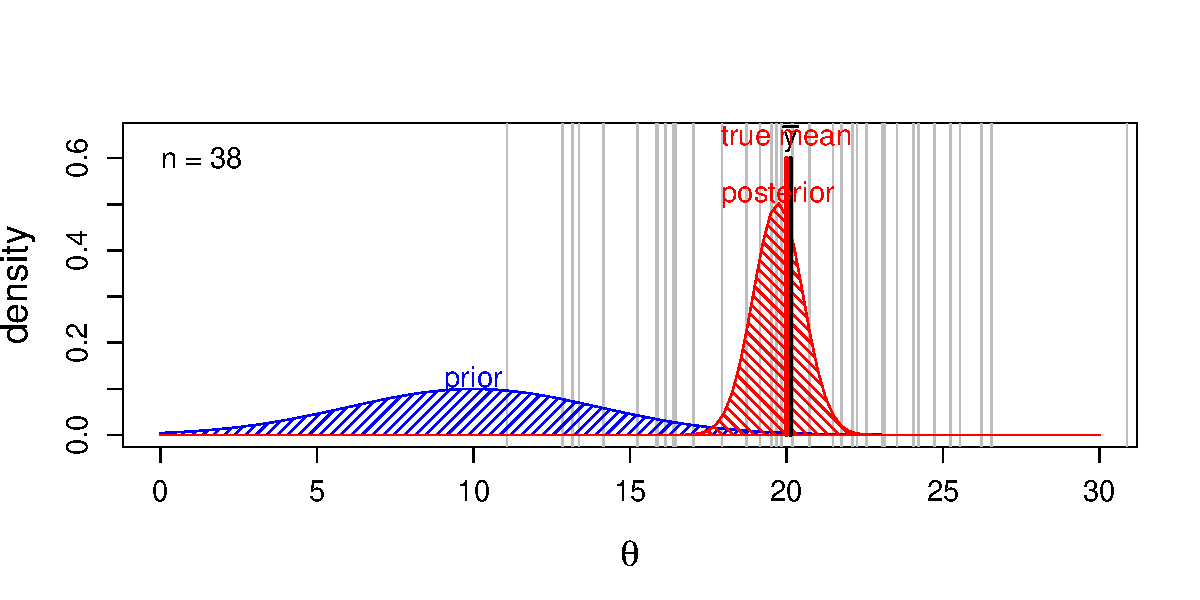
\includegraphics[width=5in]{graphics/updateExample038.pdf}}}
\mode<beamer>{\only<39>{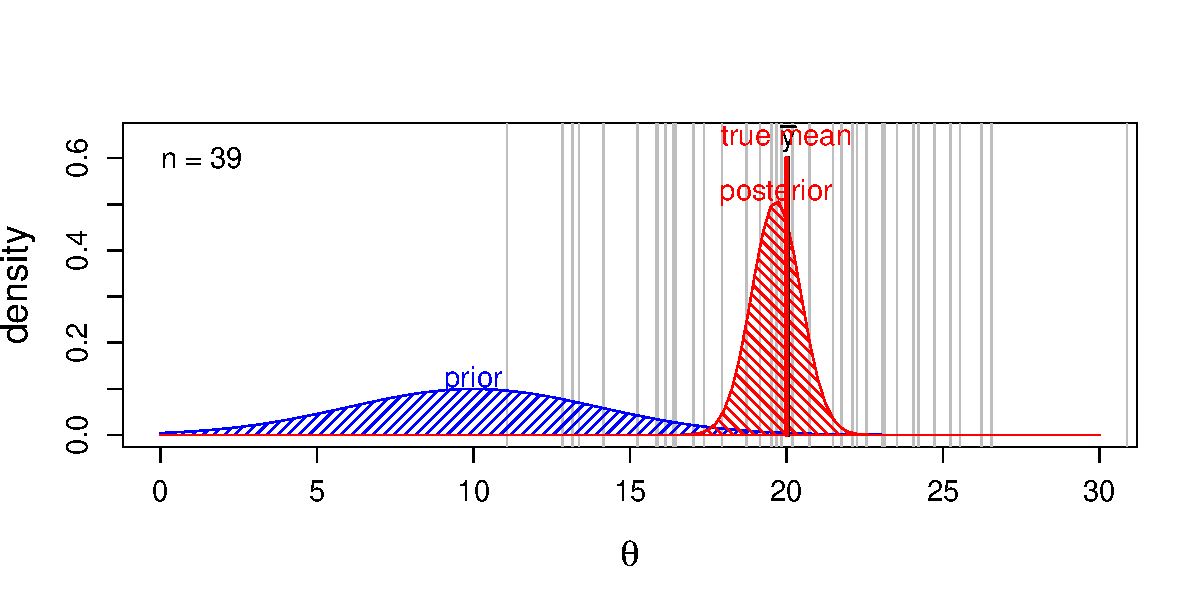
\includegraphics[width=5in]{graphics/updateExample039.pdf}}}
\mode<beamer>{\only<40>{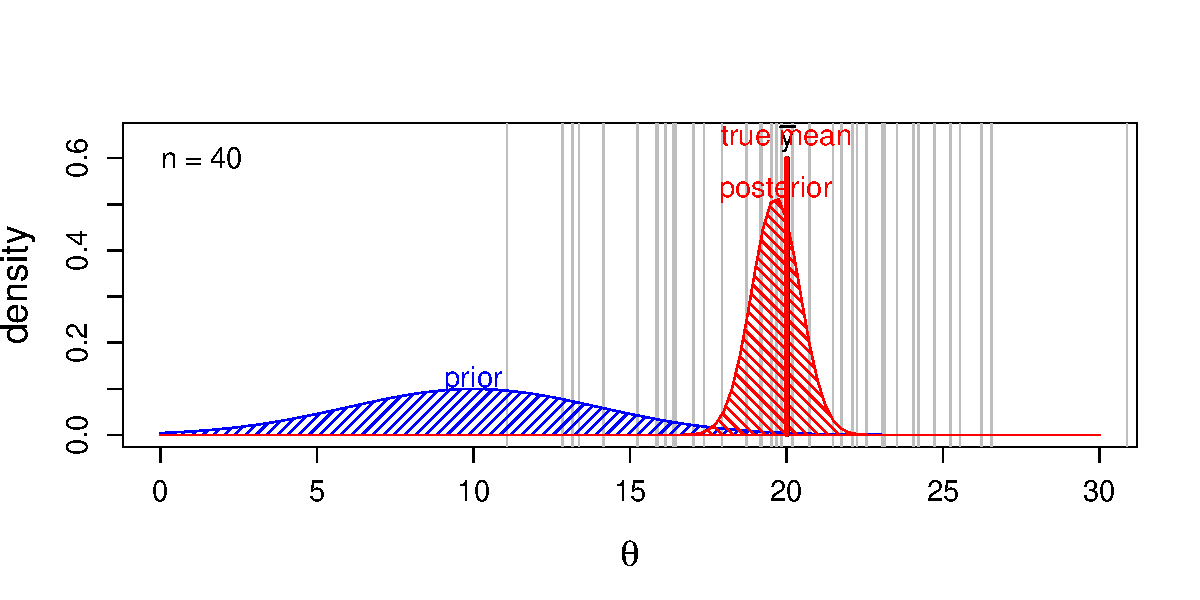
\includegraphics[width=5in]{graphics/updateExample040.pdf}}}
\mode<beamer>{\only<41>{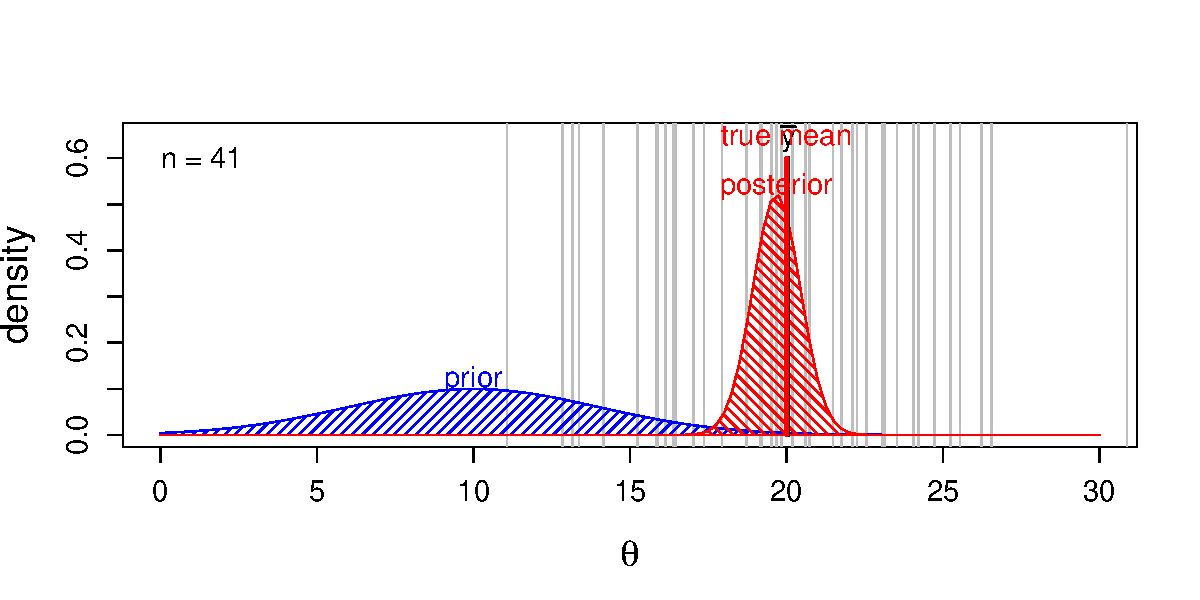
\includegraphics[width=5in]{graphics/updateExample041.pdf}}}
\mode<beamer>{\only<42>{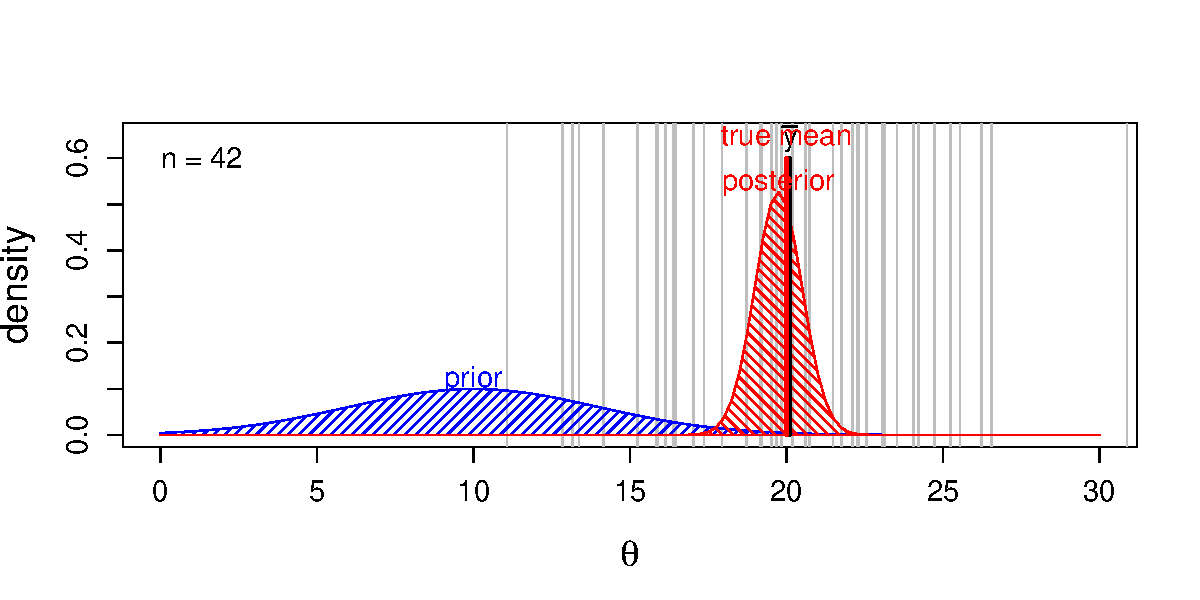
\includegraphics[width=5in]{graphics/updateExample042.pdf}}}
\mode<beamer>{\only<43>{\includegraphics[width=5in]{graphics/updateExample043.pdf}}}
\mode<beamer>{\only<44>{\includegraphics[width=5in]{graphics/updateExample044.pdf}}}
\mode<beamer>{\only<45>{\includegraphics[width=5in]{graphics/updateExample045.pdf}}}
\mode<beamer>{\only<46>{\includegraphics[width=5in]{graphics/updateExample046.pdf}}}
\mode<beamer>{\only<47>{\includegraphics[width=5in]{graphics/updateExample047.pdf}}}
\mode<beamer>{\only<48>{\includegraphics[width=5in]{graphics/updateExample048.pdf}}}
\mode<beamer>{\only<49>{\includegraphics[width=5in]{graphics/updateExample049.pdf}}}
\mode<beamer>{\only<50>{\includegraphics[width=5in]{graphics/updateExample050.pdf}}}

\end{frame}

%\subsection{The likelihood principle}

\begin{frame}<article>{The likelihood principle}

The likelihood function $p\left(y | \theta\right)$ contains all the information in the observed data $y$ from an experiment relevant to inferences about the parameter $\theta$.
\onslide<2->{
\begin{itemize}
\item  Follows directly from Bayes Rule and Bayesian inference.
\item Basically it says that inferences should be based on what is observed, not on what might have been observed.
\item Key distinction from frequentist principles and methods.
\item Has important practical consequences for clinical trial design and analysis.
\begin{itemize}
\item Removes many frequentist restrictions/penalties on:
\begin{itemize}
\item Interim analyses.
\item Interim design changes, e.g., adaptive dose assignment.
\end{itemize}
\end{itemize}
\end{itemize}
}
\onslide<3>{\alert{Caution: How the data is collected is still relevant. For example randomization is still a necessary element of experimental design for assuring exchangeability and validity of causal inference.}}

\end{frame}

\section{Computation for Bayesian modeling}

\begin{frame}
  \frametitle{Computation for Bayesian modeling}

  \begin{itemize}
  \item Full Bayesian analysis requires:
    \begin{itemize}
    \item Characterization of the joint posterior distribution of
      model parameters and of predicted outcomes.
    \item Integration of that joint posterior distribution to
      calculate quantities required for statistical inferences.
    \end{itemize}
  \item For most realistic problems, those are very computationally
    demanding tasks.
  \item Increases in computation speed and development of new
    algorithms over the last 25--30 years have finally made full
    Bayesian analysis a feasible option for routine data analysis.
  \end{itemize}
  
\end{frame}

\subsection{Maximum a Posteriori (MAP) Bayes}

\begin{frame}
  \frametitle{Maximum a Posteriori (MAP) Bayes}

  \begin{itemize}
  \item The set of model parameter values that maximize the posterior
    distribution (aka posterior mode) are called the MAP Bayes
    parameter estimates.
  \item MAP Bayes estimation is a useful approximate Bayesian method.
  \item It is strongly analogous to maximum likelihood (ML)
    estimation.
  \item ML estimation tools can often be adapted to calculate MAP
    Bayes estimates.
  \end{itemize}

\end{frame}

\begin{frame}<article>[shrink]
  \frametitle{\large Recall the NONMEM Maximum Likelihood Objective Function}

  \begin{itemize}
  \item For Single-Subject Data
$$OF_{ML}(x,\theta,\sigma^2) = \sum_{j=1}^{n}\left[\frac{y_j - f(x_j,\theta))^2}{\sigma^2} + \log\sigma^2\right]$$
\item For Population Data
  \begin{itemize}
  \item Individual
$$ -2\log L_i(Y_i|x_i,\theta,C_i) = OF_i(x_i,\theta,C_i) = \sum_{j=1}^{n_i}\left[y_j - f(x_j,\theta))^TC_i^{-1}(y_j-f(x_j,\theta))\right]+\log(\text{det}C_i)$$
\item Population
$$ -2\log L(Y|x,\theta,C) = OF(x,\theta,C) = \sum_{i=1,j=1}^{N,n_i}\left[y_{ij}-f(x_{ij},\theta))^TC_i^{-1}(y_{ij}-f(x_{ij},\theta))\right] + \sum_{i=1}^N\log(\text(det)C_i) $$
\item Individual Variance-Covariance Matrix
\begin{columns}
\column{0.5\textwidth}
$$ C_i = G_i\Omega G_i^T + H_i\Sigma H_i^T$$
\column{0.8\textwidth}
\begin{itemize}
\item $G_i$ is a matrix of partial derivatives of
  $f_{ij}(\theta,x_{ij})$ with respect to $\eta$
\item $\Omega$ is a populatoin inter-individual covariance matrix
\item $H_i$ is a matrix of partial derivatives of
  $f_{ij}(\theta, x_{ij})$ with respect to $\epsilon$
\item $\Sigma$ is a covariance matrix for residual error, $\epsilon$
  (usually diagonal)
\end{itemize}
\end{columns}
\end{itemize}
\end{itemize}

\end{frame}

\begin{frame}<article>
  \frametitle{Individual MAP (Maximum a Posteriori) Bayes Estimation}
  
(e.g. NONMEM POSTHOC or Conditional Estimation Methods)

\begin{itemize}
\item Individual parameter estimates may dominate even when data are very sparse. The balance is affected by relative magnitude of inter-individual covariance ($\Omega$) and residual variance ($\sigma^2$). 
\begin{itemize}
\item Data Dominated Estimate ($\Omega \gg sigma^2$)
\item Pop. Prior Dominated Estimate ($\sigma^2 \gg \Omega$)
\end{itemize}
$$ OF_{\text{POSTHOC},i} = \sum_j\left[\log \sigma^2 + (y_{ij} - M_{ij}(\theta,\eta_i))^2/\sigma^2\right] + \eta_i^\prime\Omega^{-1}\eta_i$$
\end{itemize}

\end{frame}

\begin{frame}<article>[shrink]
  \frametitle{Penalized Maximum Likelihood (so-called Frequentist
    Prior) Estimation of Population Parameters}
  
This is also a MAP Bayes estimation method

\begin{itemize}
\item Recall the population ML (-2log-likelihood) objective function:
  \begin{align*}
     -2\log L(Y|x,\theta,C) = OF(x,\theta,C) = &
     \sum_{i=1,j=1}^{N,n_i}\left[y_{ij}-f(x_{ij},\theta))^TC_i^{-1}(y_{ij}-f(x_{ij},\theta))\right] \\
     &+ \sum_{i=1}^N\log(\text(det)C_i)
  \end{align*}
... plus a -2log-Likelihood penalty
$$ + (\theta - \bar{\theta})\Gamma^{-1}(\theta - \bar{\theta})' + \mu \cdot (\log\text{det}(\Omega)+\text{tr}(\bar{\Omega}\Omega^{-1}))$$
Where:
\begin{itemize}
\item $\Gamma$ is the variance-covariance matrix of the Multivariate Normal prior distribution for population typical values
\item $\mu$ is the degrees of freedom and $\Omega$ is the mode for an inverse Wishart prior distribution for the covariance matrix of the inter-individual random effects
\end{itemize}
\item Result: Estimate posterior modes of the population parameters, constrained by prior distributions at the population level
\end{itemize}

\end{frame}

%# Empirical Bayes 

%#### Empirical Bayes methods are procedures for statistical inference in which the prior distributions are obtained from the same data set as the posterior parameter estimates (mode or full posterior distribution) 

%* Empricial Bayes Estimates may be posterior modes (MAP Bayes) of full posterior distributions

%* In NONMEM:
%    * Conditional estimates of individual random effects are Empirical Bayes Estimates (EBEs) when derived as part of the population estimation problem
%    * Conditional estimates of individual random effects are not Empirical Bayes Estimates (EBEs) when the prior is specified based on an external source of knowledge (e.g. MAXEVAL=0 POSTHOC with published population mean and variance parameters) 


\subsection{Full Bayesian analysis}

\begin{frame}
  \frametitle{Full Bayesian analysis}

  \begin{itemize}
\item Full Bayesian analysis refers to characterization of the joint
posterior distribution, not just it's mode.
\item Most Bayesian inference is based on univariate marginal
  posterior distributions of individual parameters or functions of
 those parameters.
\item That requires integration of the joint posterior distribution,
  usually over several dimensions.
  \end{itemize}

\end{frame}

\begin{frame}
  \frametitle{Full Bayesian analysis}

  \begin{itemize}
  \item If you're lucky those integrals have known analytic solutions,
    but that is rarely true for PK/PD modeling applications.
  \item For integrals in fewer dimensions, a numerical
    quadrature method might be practical. 
  \item Now imagine the computational requirements for hierarchical
    models, e.g., population PK models, with individual-specific
    parameters in the hundreds!!
  \end{itemize}

\end{frame}

\begin{frame}
  \frametitle{Posterior simulation}

  \begin{itemize}
  \item What if you could simulate samples of $\theta$ from the joint
    posterior distribution?
  \item Then you could estimate
    $E\left(f\left(\theta\right)|y\right)$ by the arithmetic mean:
$$E\left(f\left(\theta\right)|y\right) \approx \frac{1}{n}
\sum_{i=1}^n f\left(\theta_i\right)$$
\item More generally, you could characterize the properties of any
  marginal posterior distribution of a model parameter or function of
  model parameters, e.g., moments, quantiles, ...
\item But how do you simulate samples from a high dimensional joint
  posterior distribution?
\item Markov chain Monte Carlo (MCMC) simulation via NONMEM is one
  approach we will explore today.
\end{itemize}

\end{frame}

\begin{frame}{Inferences from posterior simulations}

  \begin{itemize}
  \item Posterior simulation yields vectors of parameters and/or
    predictions from a joint posterior distribution
  \item Marginal distributions
    \begin{itemize}
    \item To describe the posterior distribution of any scalar
      function of the parameters apply the function to each simulated
      vector. The empirical distribution of those values approximates
      the posterior distribution.
    \item The marginal distribution of any single parameter is just a
      special case of that approach.
    \end{itemize}
  \item Inferences are usually based on moments, probabilities or
    percentiles from marginal posterior distributions. They are
    readily estimated from the corresponding sample statistics for the
    simulated values.
  \end{itemize}

\end{frame}

\subsection{Markov chain Monte Carlo (MCMC) simulation}

\begin{frame}{Tools for Bayesian modeling \& inference}

  \begin{itemize}
  \item There remains the challenge of simulating from high
    dimensional posterior distributions.
  \item Markov chain Monte Carlo (MCMC) simulation has become the
    primary method.
    \begin{itemize}
    \item Simulation methods for performing high dimensional
      simulation required for Bayesian modeling.
    \item Simulate random variables from the posterior distributions
      of interest, e.g., means and variances of the population
      distributions of PK/PD parameters.
    \item Inferences follow directly from the distributions of
      simulated parameter values
      \begin{itemize}
      \item Point estimates from mean, median or mode.
      \item Posterior intervals from percentiles, e.g., 95\% interval
        from the 2.5 and 97.5 percentiles.
      \end{itemize}
    \end{itemize}
  \end{itemize}

\end{frame}

\begin{frame}{Markov Chain Monte Carlo (MCMC) simulation}

\begin{itemize}
\item Involves random draws from approximate distributions and then correcting those draws to better approximate the joint posterior.
\item The samples are drawn sequentially so that each draw depends on the previous one, thus forming a Markov chain.
\item Eventually the Markov chain converges (in distribution) to a stationary distribution that is the joint posterior distribution.
\item Algorithms for MCMC include:
\begin{itemize}
\item Metropolis-Hastings algorithm
\item Gibbs sampling
\item Hamiltonian Monte Carlo (HMC) simulation
\end{itemize}
\item MCMC samples are serially correlated:
\begin{itemize}
\item Inferences based on MCMC require more samples than would be required for independent samples
\end{itemize}
\item Practical consequences:
\begin{itemize}
\item Use only samples drawn after convergence is achieved, i.e., discard samples from a “warmup” phase.
\item Draw more samples than you would for independent random draws.
\end{itemize}
\end{itemize}

\end{frame}

\begin{frame}
  \frametitle{Gibbs sampling}
  
\begin{itemize}
\item In most cases a convergent Markov chain may be constructed by progressively sampling from the univariate full conditional distributions:
\begin{eqnarray*}
\theta_1^i &\sim& p\left(\theta_1|\theta_2^{i-1},\theta_3^{i-1},\ldots,\theta_n^{i-1},y\right) \\
\theta_2^i &\sim& p\left(\theta_2|\theta_1^i,\theta_3^{i-1},\ldots,\theta_n^{i-1},y\right) \\
& & \vdots \\
\theta_n^i &\sim& p\left(\theta_n|\theta_1^i,\theta_2^i,\ldots,\theta_{n-1}^i,y\right) \\
\end{eqnarray*}
\item This reduces the multivariate posterior sampling problem to a sequence of more manageable univariate sampling problems.
\end{itemize}

\note{The full conditional distributions are readily derived from the joint distributions.}

\end{frame}

\begin{frame}<article>
  \frametitle{Gibbs sampling example}

\begin{itemize}
\item Data: single observation from a bivariate normal distribution: $y = \left(y_1, y_2\right) \sim N\left(\mu, \Sigma\right)$
\item Unknown mean: $\mu = \left(\mu_1, \mu_2\right)$
\item Known covariance matrix: $\Sigma = \left(\begin{array}{cc} 1 & \rho \\ \rho & 1 \end{array}\right)$
\item Improper uniform prior on $\mu$
\item The conditional posterior distributions of $\mu_1$ and $\mu_2$ are:
\end{itemize}
\begin{eqnarray*}
\mu_1|\mu_2,y &\sim& N\left(y_1+\rho\left(\mu_2-y_2\right),1-\rho^2\right) \\
\mu_2|\mu_1,y &\sim& N\left(y_2+\rho\left(\mu_1-y_1\right),1-\rho^2\right) 
\end{eqnarray*}

\end{frame}

\begin{frame}<article>[fragile]
  \frametitle{Gibbs sampling example}

\begin{itemize}  
\item $y = (0, 0)$ and $\rho = 0.8$
\item For this simple case Gibbs sampling can be done with the following short R function (See R script “gibbs.example.R”):
\end{itemize}
\begin{lstlisting}[frame=single]
gibbs1 = function(nsamp,y,sigma2,mu.init){
## Gibbs sampler for bivariate normal mean with
## known covariance matrix (sigma2), an improper
## uniform prior and given one data point (y)
   mu = matrix(double(2*nsamp),ncol=2)
   mu[1,] = mu.init
   for(i in 2:nsamp){
      mu[i,1] = rnorm.cond(1,1,y,sigma2,mu[i-1,])
      mu[i,2] = rnorm.cond(1,2,y,sigma2,mu[i,])
   }
   mu
}
\end{lstlisting}

\end{frame}

\begin{frame}<article>
  \frametitle{Gibbs sampling example}
  
4 chains with different starting points

\vspace{0.5in}
\hspace{0.35in} 10 samples per chain \hspace{0.9in} 1000 samples per chain \\
\vspace{-0.5in}
\includegraphics[width=2.4in]{graphics/gibbsSamplingExample001.pdf}
\includegraphics[width=2.4in]{graphics/gibbsSamplingExample002.pdf}

\end{frame}

\begin{frame}
  \frametitle{Metropolis-Hasting algorithm}
  
  \begin{itemize}
  \item The Metropolis-Hastings is a general purpose multivariate MCMC
    algorithm.
\item It requires selection of a conditional proposal density
  $q\left(y|x\right)$ that is easy to sample from.
\item To generate $x^{(t+1)} \sim f$ given a previous value $x^{(t)}$:
\vspace{-12pt}
\textcolor{blue}{
  \begin{algorithmic}[1]
  \STATE Generate $y_t \sim q\left(y|x^{(t)}\right)$.
\STATE $x^{(t+1)} = \left\{\begin{array}{ll}
    y_t, & \text{with probability } \rho\left(x^{(t)}, y_t\right) \\
    x^{(t)}, & \text{with probability } 1 - \rho\left(x^{(t)}, y_t\right) 
	\end{array} \right.$ \\
where $\displaystyle \rho\left(x, y\right) =
\text{min}\left\{\frac{f(y)}{f(x)}\frac{q(x|y)}{q(y|x)}, 1\right\} $
  \end{algorithmic}
}
  \end{itemize}

\end{frame}

\begin{frame}[shrink]
  \frametitle{Hamiltonian Monte Carlo (HMC) simulation}
  
  Physical analogy to motivate HMC
  \begin{itemize}
  \item In classical mechanics the Hamiltonian equations describe the
    evolution of a system over time.
  \item The state of the system is described in terms of kinetic
    energy as a function of momentum (mass $\times$ velocity) and
    potential energy as a function of position.
  \item For the analogy equate the model parameters $\theta$ to
    position and equate a set of auxiliary parameters $\rho$ to
    momentum.
  \item Now define a Hamiltonian in terms of the joint posterior
    distribution of $\theta$ and $\rho$:
    \begin{align*}
      H(\theta, \rho) &= -\log\left(p\left(\theta, \rho | y\right)\right) 
                      = -\log\left(p\left(\theta | y\right)
                        p\left(\rho | \theta, y\right)\right) \\
                      &= -\log\left(p\left(\theta | y\right)\right)
                        - \log\left(p\left(\rho | \theta,
                        y\right)\right) \\
                      &= V\left(\theta\right) + T\left(\rho |
                        \theta\right) \\
      V\left(\theta\right) &= -log\left(p\left(\theta | y\right)\right)
                             = \text{potential energy} \\
      T\left(\rho | \theta\right) &= - log\left(p\left(\rho | \theta,  y\right)\right) = \text{kinetic energy}
    \end{align*}
  \end{itemize}

\end{frame}

\begin{frame}
  \frametitle{Hamiltonian Monte Carlo (HMC) simulation}
  
  \begin{itemize}
  \item $\theta$ is what we really care about.
  \item $\rho$ allows the use of Hamiltonian mechanics to more
    efficiently move through the relevant parts of the parameter
    space.
  \item Usually the distribution of $\rho$ is chosen to be independent of
    $\theta$, e.g.,
    $p(\rho | \theta) = p(\rho) = N\left(0, \Sigma\right)$.
  \item Suppose we place a frictionless particle on the potential
    energy surface $\left(-log\left(p\left(\theta |
          y\right)\right)\right)$ at some position $\theta^{t-1}$.
    \begin{itemize}
    \item We give it a shove that imparts a momentum $\rho^{t-1}$ to that
      particle at time $t-1$.
    \item The particle moves over that surface according to
      Hamiltonian dynamics.
    \item Now stop the particle at time $t$ and measure its
      position $\theta^t$.
    \item Now randomly sample a new momentum from $p(\rho)$ and give
      the particle another shove, and so on...
    \end{itemize}
  \end{itemize}

\end{frame}

\begin{frame}
  \frametitle{Hamiltonian Monte Carlo (HMC) simulation}
  
  \begin{itemize}
  \item Though the initial momentum at each step is random, the
    subsequent path will favor regions of lower potential energy
    (higher probability density).
%  \item Thus the particle will spend more time in high probability
%    regions than in low probability ones.
  \item The set of sampled positions are distributed according to the
    target posterior density.
  \item In practice the Hamiltonian equations are solved
    numerically. As a result some error is introduced in the estimated
    path.
  \item A Metropolis step is used to assure that the position samples
    converge in distribution to the target distribution.
  \end{itemize}

\end{frame}

\begin{frame}
  \frametitle{The HMC algorithm}
  
Repeat the following steps:
  \begin{enumerate}
  \item Sample  $\rho^{t-1} \sim N\left(0, \Sigma\right)$
\item Simultaneously update $\theta$ and $\rho$ by numerically solving
  the Hamiltonian equations using the leapfrog method to generate a
  proposal $\theta^*$ for $\theta^t$.
\item Apply a Metropolis step to decide whether to
  accept or reject the proposal $\theta^*$ as $\theta^t$.
  \end{enumerate}

\end{frame}

\begin{frame}
  \frametitle{The leapfrog method}

Using the starting values $\theta^{t-1}$ and $\rho^{t-1}$ the leapfrog
algorithm alternates half-step updates of $\rho$ with full step
updates of $\theta$:
\begin{align*}
  \rho &\leftarrow \rho - \frac{\epsilon}{2} \frac{\partial V}{\partial
  \theta} = \rho + \frac{\epsilon}{2} \frac{d\log\left(p\left(\theta |
         Y\right)\right)}{d\theta} \\
\theta &\leftarrow \theta + \epsilon \Sigma \rho \\
  \rho &\leftarrow \rho - \frac{\epsilon}{2} \frac{\partial V}{\partial
  \theta} = \rho + \frac{\epsilon}{2} \frac{d\log\left(p\left(\theta |
         Y\right)\right)}{d\theta} 
\end{align*}
For each HMC iteration repeat this $L$ times to yield the proposal
values $\theta^*$ and $\rho^*$.

\end{frame}

\begin{frame}
  \frametitle{The Metropolis step}
  
  \begin{itemize}
  \item Compute the ratio:
    \begin{align*}
      r &= \exp\left(H\left(\theta^{t-1}, \rho^{t-1}\right) -
          H\left(\theta^*, \rho^*\right)\right) \\
        &= \frac{p\left(\theta^* | y\right) p\left(\rho^*\right)}{p\left(\theta^{t-1} | y\right) p\left(\rho^{t-1}\right)}
    \end{align*}
  \item Accept/reject step:
     $$ \theta^t = \left\{\begin{array}{ll}
                            \theta^*, & \text{with probability} \min\left(r, 1\right) \\
                            \theta^{t-1}, & \text{otherwise}
                          \end{array} \right. $$
\item Since $\rho$ is sampled independently of
                        $\theta$ and previous values of $\rho$, we
                        just discard $\rho^*$ and sample a new value
                        for the next HMC iteration.
\end{itemize}

\end{frame}

\begin{frame}
  \frametitle{HMC algorithm parameters}
  
Parameters that must be set: discretization time $\epsilon$, number of
leapfrog steps $L$ and mass matrix $\Sigma^{-1}$.\\ \ \\
Sampling efficiency is very sensitive to those parameters:
\begin{itemize}
\item $\epsilon$ too large $\rightarrow$ too many proposals rejected
\item $\epsilon$ too small $\rightarrow$ long simulation times
\item $L$ too large $\rightarrow$ too much work for each iteration
\item $L$ too small $\rightarrow$ devolves to a random walk
\item If $\Sigma^{-1}$ is poorly tuned to the problem, $\epsilon$
  needs to be decreased and $L$ increased to maintain precision and efficiency. 
\end{itemize}
Stan automatically optimizes those parameters using the NUTS (no
U-turn sampling) algorithm \cite{hoffman2014}. 

\end{frame}

\begin{frame}
  \frametitle{HMC performance}
  
  \begin{center}
    \includegraphics[width=0.9\textwidth]{graphics/samplingCompare2.pdf}
  \end{center}
{\scriptsize from RM Neal. MCMC Using Hamiltonian Dynamics (2011) \cite{neal2011}}

\end{frame}

\begin{frame}
  \frametitle{HMC performance}
  
  \begin{center}
    \includegraphics[width=0.9\textwidth]{graphics/samplingCompare1.pdf}
  \end{center}
{\scriptsize from MD Hoffman and A Gelman. The no-U-turn
  sampler: Adaptively setting path lengths in Hamiltonian Monte Carlo
  (2014) \cite{hoffman2014}}

\end{frame}

\begin{frame}
  \frametitle{HMC issues/limitations}
  
  \begin{itemize}
  \item Requires calculation of the gradient
    $\frac{d\log\left(p\left(\theta | Y\right)\right)}{d\theta}$
  \item Suitable for sampling of continuous parameters only
    \begin{itemize}
    \item Cannot sample discrete parameters
    \item Discrete data is OK as long as the likelihood depends only
      on continuous parameters.
    \item Models with discrete parameters, e.g., finite mixture
      models, can often be implemented by marginalizing out the
      discrete parameters.
    \end{itemize}
  \end{itemize}

\end{frame}

\section{Overview of NONMEM implementations}

\begin{frame}
  \frametitle{Overview of NONMEM implementations}
  
  \begin{itemize}
  \item MAP estimation
    \begin{itemize}
    \item Using prior distributions with any optimization method
    \end{itemize}
  \item MCMC
    \begin{itemize}
    \item METHOD = BAYES: Metropolis-Hastings within Gibbs sampling
    \item METHOD = NUTS: No U-turn sampler (HMC with automatic
      optimization of sampling parameters)
    \end{itemize}
  \end{itemize}

\end{frame}

\begin{frame}
  \frametitle{Prior specification in NONMEM}
  
  \begin{itemize}
  \item THETA: (multivariate) normal distribution
  \item OMEGA \& SIGMA: inverse Wishart
    \begin{itemize}
    \item NUTS also supports
      \begin{itemize}
      \item lognormal or half-t distributions for SDs, i.e., square
        roots of the diagonal elements of OMEGA or SIGMA
      \item LKJ distribution for the correlation matrix
      \end{itemize}
    \end{itemize}
    \end{itemize}

  \end{frame}

  \begin{frame}<article>
    \frametitle{Some NONMEM bugs/issues involving BAYES \& NUTS}

    \begin{itemize}
    \item The THIN option does not work correctly with the FORTRAN
      write statements when using parallel computation
      \begin{itemize}
      \item Only thins the samples for the first file, e.g., ipar1.txt
      \end{itemize}
    \item NUTS also does not work correctly with the FORTRAN write
      statements when using parallel computation
      \begin{itemize}
      \item Creates only the first file.
      \item Writes multiple records for each individual-iteration
        combination; there should only be one. In addition the records
        are not always the same; they should be.
      \end{itemize}
    \item Supposedly you can specify truncated priors by constraining
      the initial estimates, but in our hands most runs using such
      constraints fail.
      \begin{itemize}
        \item Attempts to ``bullet-proof'' the code didn't seem to help,
        e.g., combining constraints with statements that test for
        violations of the constraints and execute EXIT when a
        violation occurs combined with the NOABORT option.
      \end{itemize}
    \end{itemize}
    
  \end{frame}

\section{Hands-on 1: Example illustrating Bayesian data analysis workflow}

\begin{frame}
  \frametitle{Hands-on 1: Example illustrating Bayesian data analysis workflow}
  \framesubtitle{Modeling workflow using NONMEM \& R}
  
We will use R to implement data analysis workflows:
\begin{itemize}
\item Data management
\item Launching NONMEM via R functions
\item Summarizing and analyzing the MCMC samples generated by NONMEM
  \begin{itemize}
  \item Tabulation of parameter estimates using an RStan function
\item Graphical diagnostics and summaries using functions from the bayesplot package
\item Posterior predictive checking via R code and ggplot2 plots
  \end{itemize}
\end{itemize}

\end{frame}

% R packages & functions: rstan, bayesplot, functions in stanTools.R
% Walk through R script 
% Also briefly show Rmd example

\begin{frame}
  \frametitle{NONMEM workflow example}
  \framesubtitle{\large PK-PD modeling of time-averaged biomarker and
    PK data}
  
  \begin{itemize}
  \item Phase 1 single dose study in healthy volunteers
    \begin{itemize}
    \item Parallel dose-escalation design
    \item 8 subjects per dose arm
    \item Single doses of ME-2
      \begin{itemize}
      \item Placebo, 1.25, 5, 10, 15, 20, 30, 40, 60 and 80 mg
      \end{itemize}
    \item PK: plasma concentrations of parent drug
    \item Biomarker: ex vivo inhibition of factor Xa activity in
      plasma
      \begin{itemize}
      \item PK and biomarker measured at 0, 0.083, 0.167, 0.25, 0.5,
        0.75, 1, 1.5, 2, 3, 4, 6, 8, 12, 18 and 24 hours after dose.
      \end{itemize}
    \end{itemize}
  \item Hands-on exercise:
    \begin{itemize}
    \item Model relationship between time-averaged factor Xa
      inhibition and time-averaged ME-2 plasma concentrations
    \end{itemize}
  \end{itemize}

\end{frame}

\begin{frame}
  \frametitle{EDA: PK and biomarker data}

\vspace{-0.1in}  
\includegraphics[width=2.3in]{graphics/FXaPKBiomarkerPlots001.pdf}
\includegraphics[width=2.3in]{graphics/FXaPKBiomarkerPlots002.pdf}

\end{frame}

\begin{frame}
  \frametitle{EDA: Relationship between biomarker and PK data}
  
\vspace{-0.1in}  
\includegraphics[width=2.3in]{graphics/FXaPKBiomarkerPlots003.pdf}
\includegraphics[width=2.3in]{graphics/FXaPKBiomarkerPlots005.pdf}

\end{frame}

\begin{frame}
  \frametitle{Model}
  
\begin{itemize}
\item Sigmoid Emax model relating time-averaged \% inhibition of factor Xa activity to time-averaged ME-2 plasma concentration in the $i^{th}$ subject:
\begin{eqnarray*}
\overline{E}_{24,i} &\sim& N\left(\hat{E}_{24,i},\sigma\right) \\
\hat{E}_{24,i} &=& \frac{E_{max} \overline{c}_{24,i}^\gamma}{EC_{50}^\gamma + \overline{c}_{24,i}^\gamma}
\end{eqnarray*}
\item Weakly informative prior distributions:
  \begin{align*}
    \text{logit}\left(\frac{E_{max}}{100}\right) &\sim N\left(0,
                                                   \sqrt{2}\right) \\
    \log\left(EC_{50}\right)  &\sim N\left(\log(245), 1\right) \\
\log\left(\gamma\right) &\sim N\left(\log(2.1), \sqrt{0.5}\right) \\
\log\left(\sigma\right) &\sim N\left(\log(10), 1\right)
  \end{align*}
%  \begin{eqnarray*}
%E_{max} &\sim& U\left(0, 100\right) \\
%EC_{50}  &\sim& \text{half-}N\left(0, 250\right) \\
%\gamma &\sim& \text{half-}N\left(0, 5\right) \\
%\sigma &\sim& \text{half-Cauchy}\left(0, 10\right)
%\end{eqnarray*}
\end{itemize}
{\scriptsize See \cite{gelman2006} for half-Cauchy rationale.}

\end{frame}

\begin{frame}
  \frametitle{Files}
  
  \begin{itemize}
  \item Data: data/derived/fxa.data.avg.csv
  \item MAP
    \begin{itemize}
    \item NONMEM model: model/fxaInhibitAvgMAPstub.ctl
    \item Rmd file: script/fxaInhibitAvgMAP.Rmd
    \end{itemize}
  \item BAYES (Gibbs / Metropolis-Hastings)
    \begin{itemize}
    \item NONMEM model: model/fxaInhibitAvgBAYESstub.ctl
    \item Rmd file: script/fxaInhibitAvgBAYES.Rmd
    \end{itemize}
  \item NUTS
    \begin{itemize}
    \item NONMEM model: model/fxaInhibitAvgNUTSstub.ctl
    \item Rmd file: script/fxaInhibitAvgNUTS.Rmd
    \end{itemize}
  \end{itemize}

\end{frame}

\section{Prior distributions}

\begin{frame}
  \frametitle{Brief discussion on prior distributions}

  \begin{itemize}
  \item Think of prior distributions as part of the model.
\item Priors should be chosen and 
subjected to scrutiny much like other model components.
\item Model checking should ideally include sensitivity analysis of
  the priors.
\item Choice of priors is most critical with sparse or limited data.
  \end{itemize}

See \url{https://github.com/stan-dev/stan/wiki/Prior-Choice-Recommendations}

\end{frame}

\begin{frame}
  \frametitle{What is the function of a prior distribution}

  \begin{itemize}
  \item<1-> Represent prior knowledge
\item<2-> Regularization to facilitate computation
  \begin{itemize}
 \item Typically weakly-moderately informative
\item E.g., Cauchy with most of its mass in a plausible range, but heavy tails allow for diagnosis of prior-posterior discrepancies.
  \end{itemize}
  \end{itemize}

\end{frame}

\begin{frame}
  \frametitle{What does it mean to be informative, uninformative or
    weakly informative?}
  
Not well defined, but here's an attempt at some loose definitions:
  \begin{itemize}
  \item<1-> Weakly informative prior: A prior that rules out unreasonable
    parameter values but is not so strong as to rule out values that
    might make sense
\item<2-> Informative prior: A prior that purposely represents
  information intended to influence the  posterior distribution
  \begin{itemize}
  \item To capture prior knowledge
\item To challenge the analysis with competing points of view, e.g.,
  use of pessimistic or optimistic priors.
  \end{itemize}
\item<3-> Uninformative prior: Ostensibly a prior that represents no
  information and therefore ``let's the data tell the story.''
  \begin{itemize}
  \item E.g., a constant over the entire real line---an improper prior
  \end{itemize}
  \end{itemize}

\end{frame}

\begin{frame}
\frametitle{Beware: That ``uninformative'' prior might not be!}

\begin{itemize}
\item Suppose you use an improper prior for a standard deviation---a
  constant over the positive real line.
\item That means all positive values are equally likely. Sounds like a
  reasonable definition of uninformative doesn't it?
\item But that means that the prior assigns infinitely more
  probability to the set of values greater than any fixed value you care to
  choose.
\item This will tend to bias the posterior to high values.
\item Bottom line: A uniform distribution does not automatically
  confer uninformativeness.
\end{itemize}

\end{frame}

\begin{frame}<article>
  \frametitle{More on NONMEM prior specification}
  


\end{frame}

\section{Hands-on 2: MAP popPK with selective use of informative priors}

\begin{frame}
  \frametitle{Hands-on 2: MAP popPK with selective use of informative
    priors for nuisance parameters: pediatric atorvastatin}

\begin{center}
\includegraphics[width=\textwidth]{graphics/KnebelTitle.png}
\end{center}  

\end{frame}

\begin{frame}
  \frametitle{The scenario}

  \begin{itemize}
  \item Sparse PK sampling in 39 pediatric patients.
\item Previous popPK model for adult patients used a 2 compartment
  model with first order absorption for parent drug.
\item Pediatric data alone was not sufficient to estimate all
  parameters of that model.
\item The choice:
  \begin{itemize}
  \item Simplify the model to the point where all parameters are
    estimable.
\item Retain the more complete model and borrow information from the adult model with appropriate scaling.
  \end{itemize}
  \item Knebel et al chose a cautious form of the latter:
    \begin{itemize}
    \item Informative priors based on the adult model, but only for 2
      parameters that are not crucial for the inferences of interest,
      $k_a$ and $V_3$.
    \end{itemize}
  \end{itemize}

Assignment: replicate that analysis using MAP Bayes estimation

\end{frame}

\begin{frame}
  \frametitle{The model}

\begin{columns}
\column{0.5\textwidth}
\includegraphics[width=\textwidth]{graphics/KnebelModel.png}
\column{0.5\textwidth}
We will limit our exercise to the parent drug.
\begin{itemize}
\item 2 compartment model with 1st order absorption (ADVAN4 TRANS4)
\item Normal residual variation with SD proportional to predicted
  concentration ($c_{\text{obs},i} \sim N\left(\widehat{c}_i,
    \widehat{c}_i sigma\right)$)
\item Informative prior distributions for $k_a$ and $V_3$
\item Weakly informative priors for the remaining parameters
\end{itemize}
\end{columns}

\end{frame}

\begin{frame}
  \frametitle{The model}

\begin{footnotesize}
  \begin{align*}
    \log\left(\{\widehat{CL/F}, \widehat{V_2/F}, Q/F, k_a,
    V_3/F\}\right) \sim\ &
                                                        N\left(\{5.65,
                                                        5.60, 4.29,
                                                        -1.33, 7.07\},\right. \\
                                                        & \left.\{12, 12, 12,
                                                        0.00684,
                                                        0.0156\}\right)
    \\
    \log\left(\{CL/F_i, V_2/F_i\}\right) \sim\ &
                                           N\left(\log\left(\{\widehat{CL/F},
                                           \widehat{V_2/F}\}\right),
                                           \Omega\right) \\
\Omega_{\{CL, V_2\}} \sim\ & \text{inverse Wishart}\left(\left[\begin{array}{cc}
                 0.1003 &  0.06034 \\
                  0.06034 &  0.8477
    \end{array}\right], 4\right)
  \end{align*}
\end{footnotesize}

\end{frame}

\begin{frame}
  \frametitle{Files}
  
  \begin{itemize}
  \item Data: data/derived/atorvWrkShop.csv
    \item NONMEM model: model/atorvMAPBayesstub.ctl
    \item Rmd file: script/atorvMAPBayes.Rmd
  \end{itemize}

\end{frame}

%\section{Model evaluation and comparison}

\begin{frame}<article>
  \frametitle{Bayesian model evaluation \& comparison: The ideal}

  \begin{itemize}
  \item Mixture of all possible ``true'' models including all known
    substantive information
  \item Extends the notion of Bayesian modeling of uncertainty to
    include uncertainty in model structure
  \item Under such a grand mixture model the tasks of model
    evaluation, model comparison and sensitivity analysis are all
    handled within a single analysis
    \begin{itemize}
    \item Each model in the mixture is associated with a posterior
      probability that it is the ``true'' (or ``best'') model. This provides a metric
      for comparing models.
    \item Sensitivity to model choice is obtained by comparing
      model-specific posterior predictions
    \end{itemize}
    \item Like most ideals it cannot be achieved in full, only approached via
    practical compromises
  \end{itemize}
  
\end{frame}

\begin{frame}<article>
  \frametitle{Bayesian model evaluation \& comparison}
  \framesubtitle{\large Philosophical consequences of the ideal}

  \begin{itemize}
  \item Model selection is often avoided in favor of using a
    ``fuller'' model that contains potential competing models as
    special cases
    \begin{itemize}
    \item Particularly avoided is the classic approach of performing a
      sequence of hypothesis tests
    \item The ``fuller'' model approach acknowledges and quantifies
      the uncertainty in the relative ``correctness'' of competing
      models.
    \end{itemize}
  \item Types of ``fuller'' models
    \begin{itemize}
    \item Discrete mixture models, e.g.,
      \begin{eqnarray*}
        p\left(y|\theta\right) &=& \Pr\left(M_1\right) p\left(y|\theta,M_1\right) + \Pr\left(M_2\right) p\left(y|\theta,M_2\right) +\\
        & & \cdots + \Pr\left(M_n\right) p\left(y|\theta,M_n\right) 
      \end{eqnarray*}
    \item Continuous mixture models, e.g., models containing all
      covariates of potential interest
    \end{itemize}
  \end{itemize}

\end{frame}

\begin{frame}<article>
  \frametitle{Bayesian model evaluation \& comparison}
  \framesubtitle{\large Typical practical Bayesian model development}

  \begin{itemize}
  \item Propose initial model structure based on available prior
    information.
    \begin{itemize}
    \item Realistically exploratory analysis of the new data also
      influences this process,
    \end{itemize}
  \item Assess whether model is consistent with the data and prior
    information
    \begin{itemize}
    \item Posterior predictive checking
    \item Are model inferences, predictions and values of parameters
      or other derived quantities consistent with other knowledge?
    \end{itemize}
  \item Assess sensitivity to potentially influential assumptions,
    e.g., choice of prior distributions
  \item If deficiencies are discovered that could adversely affect
    important inferences then explore model revisions and reassess as
    before.
  \end{itemize}

\end{frame}

\begin{frame}<article>
  \frametitle{Bayesian model evaluation \& comparison}
  \framesubtitle{\large Typical practical Bayesian model development
    (cont.)}

  \begin{itemize}
  \item Use the model resulting from this process for pre-planned
    inferences.
  \item Optionally there may be additional hypothesis-generating
    activities, e.g.,
    \begin{itemize}
    \item Data mining efforts to explore the influence of covariates
      not considered in the original model
    \item Further exploration of alternative model structures not
      considered in the previous sensitivity analyses
    \end{itemize}
  \end{itemize}

\end{frame}

\begin{frame}<article>
  \frametitle{Posterior predictive checking (PPC)}
  
  \begin{itemize}
  \item Graphical checks
    \begin{itemize}
    \item Comparing data \& predictions
    \item Comparing data summaries and model predictions/inferences
    \item Residuals
    \end{itemize}
  \item Formal numerical checks
    \begin{itemize}
    \item Posterior predictive p-values based on a test statistic
    \end{itemize}
  \end{itemize}

\end{frame}

\begin{frame}<article>
  \frametitle{Graphical checks: Comparing data \& predictions}
  
    Posterior medians \& 90\% prediction intervals compared to
    observed data
  \begin{center}
    \includegraphics[width=2.4in,trim=0.2in 0 0
    0,clip]{graphics/me2HandsOn2Plots011.pdf}
    \includegraphics[width=2.4in,trim=0.2in 0 0
    0,clip]{graphics/me2HandsOn2Plots024.pdf}
  \end{center}

\end{frame}

\begin{frame}<article>
  \frametitle{Graphical checks: Comparing data summaries and model predictions/inferences}
  
    Posterior densities of predicted mean peak effect and area under
    the effect curve compared to observed means.
\vspace{-0.25in}
  \begin{center}
    \includegraphics[width=2.4in,trim=0.2in 0 0
    0,clip]{graphics/me2HandsOn2Plots025.pdf}
    \includegraphics[width=2.4in,trim=0.2in 0 0
    0,clip]{graphics/me2HandsOn2Plots026.pdf}
  \end{center}

\end{frame}

\begin{frame}<article>
  \frametitle{Graphical checks: Residuals}
  
    Uncertainty in residuals and predictions can be depicted with lines representing prediction intervals
  \begin{center}
    \includegraphics[width=2.4in,trim=0.2in 0 0
    0,clip]{graphics/me2HandsOn2Plots028.pdf}
    \includegraphics[width=2.4in,trim=0.2in 0 0
    0,clip]{graphics/me2HandsOn2Plots029.pdf}
  \end{center}

\end{frame}

\begin{frame}<article>
  \frametitle{Sensitivity analysis}
  
  \begin{itemize}
  \item Generally desirable to assess sensitivity of key inferences to
    model assumptions
    \begin{itemize}
    \item True for any modeling strategy, not just Bayesian approaches
    \end{itemize}
  \item Model assumptions to be evaluated
    \begin{itemize}
    \item Model structure, i.e., functional forms of the likelihood
      and prior distribution
    \item Quantitative assumptions, i.e., values of the parameters of
      the prior distribution
    \item Let's focus on the prior distribution since that is unique
      to Bayesian modeling
    \end{itemize}
  \end{itemize}

\end{frame}

\begin{frame}<article>
  \frametitle{Sensitivity analysis: Prior distribution}
  
  \begin{itemize}
  \item When your intention is for the prior distribution to be
    non-informative
    \begin{itemize}
    \item Compare effect of different prior distributions on important
      inferences or predictions
      \begin{itemize}
      \item Different degrees of weak informativeness, e.g., normal
        distributions with various large variances
      \item Different distribution types, e.g., t-distributions with
        various degrees of freedom instead of a normal distribution
      \end{itemize}
    \end{itemize}
  \end{itemize}

\end{frame}

\begin{frame}<article>
  \frametitle{Sensitivity analysis: Prior distribution}
  
  When your intention is for the prior distribution to be informative
  \begin{itemize}
  \item Desirable to assess the relative influence of prior knowledge
    and new data on important inferences.
  \item Sensitivity to the prior distribution is not necessarily a bad
    thing, but it is desirable to know the extent to which the prior
    affects your inferences.
  \item Should explore a range of priors consistent with the range of
    knowledge and beliefs held by other stakeholders in the analysis.
  \item For example:
    \begin{itemize}
    \item When evaluating the probable benefit of some treatment,
      consider priors that reflect more or less skepticism than the
      one used for the primary analysis.
    \item If the primary analysis concludes the treatment is more
      beneficial than a comparator:
      \begin{itemize}
      \item Consider identifying the least skeptical prior that would
        make the conclusion unconvincing.
      \item Assess whether that skeptical prior is plausible.
      \end{itemize}
    \end{itemize}
  \end{itemize}

\end{frame}

\begin{frame}<article>
  \frametitle{Bayesian model comparison}
  
  \begin{itemize}
  \item Competing models may be compared with respect to the various
    modeling evaluation methods just described, i.e.,
    \begin{itemize}
    \item Posterior predictive checks
    \item Consistency with other substantive knowledge
    \end{itemize}
  \item Specific metrics for comparing models include:
    \begin{itemize}
    \item Measures of out of sample predictive accuracy \cite[Chapter 7]{gelman2014}
      \begin{itemize}
      \item Watanabe-Akaike Information Criterion (WAIC)
\item Leave one out cross validation (LOO-CV)
\item Both may be estimated from Stan output using the loo R package
  \cite{vehtari2015}.
      \end{itemize}
    \end{itemize}
  \end{itemize}

\end{frame}

\begin{frame}<article>
  \frametitle{Bayesian model comparison}
  
  \begin{itemize}
 \item Demo: Using the hands-on session example, let's compare the
  previously specified model with a model that assumes Emax = 100\%.
  \begin{itemize}
    \item Data: data/derived/fxa.data.csv
  \item Stan model 1: model/fxaInhibit1Ncp.stan
  \item R script for model 1: script/fxaInhibit1Ncp.R
  \item Stan model 2: model/fxaInhibit2Ncp.stan
  \item R script for model 2: script/fxaInhibit2Ncp.R
\item R script for model comparison: fxaInhibitModelCompare.R
  \end{itemize}
  \end{itemize}

\end{frame}

\begin{frame}<article>
  \frametitle{Other approaches not covered}
  
  \begin{itemize}
  \item Other “IC’s”, e.g., Akaike IC, Bayesian IC, Schwartz IC, …
  \item Bayes factors
    \begin{itemize}
    \item For model comparison
    \item For model averaging
    \end{itemize}
  \item Other model averaging or mixture model approaches
  \end{itemize}

\end{frame}


\section{Assessing convergence \& adequacy of sample sizes}

\begin{frame}
  \frametitle{Assessing convergence \& adequacy of sample sizes}
  
\begin{itemize}
\item Early samples may be unrepresentative of the target distribution
\item MCMC samples within a chain are autocorrelated 
\begin{itemize}
\item Inferences based on MCMC samples are less precise than those from the same number of independent samples
\item Autocorrelation also influences the rate of convergence
\end{itemize}
\end{itemize}

\end{frame}

\begin{frame}
  \frametitle{Assessing convergence \& adequacy of sample sizes}
  
\begin{columns}
\column{0.6\textwidth}
\begin{itemize}
\item Use a warmup phase, i.e., discard early iterations
\item Monitor convergence via multiple chains with different starting points
\begin{itemize}
\item Look for chains to converge to a common distribution
\item You want chain history plots to look more like straight horizontal “fuzzy caterpillars” than “wiggly snakes”
\item Monitor Gelman-Rubin diagnostics (Rhat) and/or Gelman-Rubin-Brooks plots
\begin{itemize}
\item Essentially ratios of total variance to within chain variance.
\item Should approach 1 for all parameters of interest on convergence
\end{itemize}
\end{itemize}
\end{itemize}
\column{0.4\textwidth}
\center
\vspace{-16pt}
Poor convergence \& mixing\\
\includegraphics[width=\textwidth,height=0.4\textheight]{graphics/poorConvergence.pdf}\\
\vspace{-8pt}
Good convergence \& mixing\\
\includegraphics[width=\textwidth,height=0.4\textheight]{graphics/goodConvergence.pdf}
\end{columns}

\end{frame}

\begin{frame}
\frametitle{IMHO}  

  \begin{itemize}
\item Do NOT trust automatic convergence detection to determine number
of burn-in samples. 
\item In particular, do NOT use NONMEM's termination tests (CTYPE
  option) for terminating burn in.
  \end{itemize}


\end{frame}

\begin{frame}
  \frametitle{How many samples?}
  
\begin{itemize}
\item Number of samples depends on the inference(s) of interest and the desired precision
\item For independent samples:
\begin{itemize}
\item A posterior mean of a parameter $\theta$ is estimated with an error of $\sim \frac{s_\theta}{\sqrt{n}}$ where $s_\theta$ is the standard deviation of the simulated values of $\theta$ and $n$ is the number of samples.
\item A probability $p$ is estimated with an error of $\sim \sqrt{\frac{p(1-p)}{n}}$.
\end{itemize}
\item In general more samples are required for estimating tail quantiles and probabilities than for central tendencies and probabilities near 0.5
\end{itemize}

\end{frame}

\begin{frame}
  \frametitle{How many samples?}

\vspace{-0.1in}
\begin{footnotesize}
\begin{itemize}
\item Suppose the posterior distribution of $\theta$ is $N\left(\mu = 10, \sigma = 2\right)$.
\item What if we use simulation to estimate various features of that distribution?
\item The following are bootstrap estimates of error due to simulation:
\end{itemize}
\end{footnotesize}
\vspace{-0.1in}
\includegraphics[width=2.4in]{graphics/simPrecision001.png}
\includegraphics[width=2.4in]{graphics/simPrecision002.png}

\end{frame}

\begin{frame}
  \frametitle{How many MCMC samples?}
  
\begin{itemize}
\item Given a set of MCMC samples it is possible to adjust for autocorrelation to estimate:
\begin{itemize}
\item The equivalent number of independent samples, aka effective
  sample size (n\_eff)
\item The standard error in the estimated posterior mean
\item The rstan print and summary functions provide estimates of each.
\end{itemize}
\item Guidance based on independent samples may then be applied
\end{itemize}
For more rigorous and comprehensive treatment see Robert and
  Casella 2004  and 2010 \cite{robertAndCasella2004,robertAndCasella2010}.

\end{frame}

\section[Getting posterior samples for individual parameters]{Getting
  your hands on posterior samples for individual parameters and
  predictions}

\begin{frame}
  \frametitle{Getting your hands on posterior samples for individual
    parameters and predictions}

  \begin{itemize}
  \item With METHOD = BAYES or NUTS NONMEM writes MCMC sampled
    parameter values to a file named in the \$ESTIMATION statement
    (Defaults to $<$model name$>$.ext).
  \item Only population parameters are written.
  \item Use FORTRAN WRITE statements (verbatim code) to write
    individual parameter or prediction values to files \cite[Example 8,
    pp. 277--280]{nonmem741}.
  \end{itemize}
  
\end{frame}

\section{Priors for covariance matrices (OMEGA \& SIGMA)}

\begin{frame}
  \frametitle{Priors for covariance matrices (OMEGA \& SIGMA)}

    \begin{itemize}
  \item METHOD = BAYES
    \begin{itemize}
    \item Inverse Wishart
    \end{itemize}
    \item METHOD = NUTS
      \begin{itemize}
      \item OLKJDF = 0: Inverse Wishart
       \item OLKJDF $>$ 0: LKJ distribution for the correlation matrix
         with shape parameter = OLKJDF
         \begin{itemize}
         \item OVARF $>$ 0: lognormal distribution for
           $\sqrt{\Omega_{ii}}$ where $\Omega_{ii}$ is a diagonal
           element of OMEGA parameterized as:
           $$
           \log(\sqrt{\Omega_{ii}}) \sim
           N\left(\log\left(\sqrt{\text{OmegaPrior(i,i)}}\right), \frac{1}{\text{OVARF}}\right).
           $$
         \end{itemize}
       \item OVARF $<$ 0:  half-t distribution for
           $\sqrt{\Omega_{ii}}$ where $\Omega_{ii}$ is a diagonal
           element of OMEGA parameterized as:
           $$
           \sqrt{\Omega_{ii}} \sim \text{half-}t\left(0,
             \sqrt{\text{OmegaPrior(i,i)}}, \left|OVARF\right|\right)
             $$
     \end{itemize}
    \end{itemize}

  
\end{frame}

\begin{frame}
  \frametitle{NONMEM parameterization of the inverse Wishart distribution}
  
NONMEM implementation of inverse Wishart prior for $\Omega$ (or
    $\Sigma$):
    \begin{align*}
      \Omega &\sim W^{-1}\left(\nu\Omega_\text{prior}, \nu\right) \\
W^{-1} &= \text{Standard parameterization of the inverse Wishart} \\
\nu &= \text{degrees of freedom} \\
E\left(\Omega\right) &= \frac{\nu\Omega_\text{prior}}{\nu - n - 1} \\
\text{Var}\left(\Omega_{ii}\right) &= \frac{E\left(\Omega_{ii}\right)  \left(\nu - n -
                          1\right)}{\nu} \\
n &= \text{dim}\left(\Omega\right)
    \end{align*}

\end{frame}

\begin{frame}
  \frametitle{Inverse Wishart distribution}

Guidance for setting $Omega_\text{prior}$ and $\nu$:
\begin{align*}
  \nu_i &=
  \frac{2E\left(\Omega_{ii}\right)}{\text{Var}\left(\Omega_{ii}\right)} + n
  + 3 \\
\Omega_{\text{prior},ii} &= \frac{E\left(\Omega_{ii}\right)\left(\nu_i - n -
                          1\right)}{\nu_i} \\
\end{align*}
\begin{itemize}
\item Set diagonal elements of $\Omega_\text{prior}$ to the calculated values
of $\Omega_{\text{prior},ii}$
\item Set $\nu = \text{min}\left(\nu_i\right)$.
\end{itemize}

\end{frame}

\section[Hands-on 3: Full Bayes popPK]{Hands-on 3: Full Bayes popPK with selective use of
  informative priors}

\begin{frame}
  \frametitle{Hands-on 3: Full Bayes popPK with selective use of
    informative priors for nuisance parameters: pediatric
    atorvastatin}
  
  \begin{itemize}
  \item Let's repeat the analysis of the pediatric atorvastatin data
    from the hands-on 1 example using METHOD = NUTS.
\item Incorporate some of the things we've discussed since then.
  \begin{itemize}
\item Graphical and quantitative assessment of convergence.
\item Capturing individual parameter MCMC samples.
\item Posterior predictive checking.
\end{itemize}
\item Also revise the priors:
  \begin{itemize}
  \item Add weakly informative priors for THETA(6) (log(F1chew)) \&
    THETA(7) (log(SD)).
    \item Use more reasonable weakly informative priors for THETA(1),
      THETA(2) \& THETA(3)
      \item Use lognormal priors for diag(OMEGA) and LKJ for IIV
        correlation matrix.
  \end{itemize}
  \end{itemize}

\end{frame}

\begin{frame}
  \frametitle{Files}
  
  \begin{itemize}
  \item Data: data/derived/atorvWrkShop.csv
    \item NONMEM model: model/atorv1stub.ctl
    \item Rmd file: script/atorv1.Rmd
  \end{itemize}

\end{frame}

\section{When stuff goes wrong}

\begin{frame}
  \frametitle{When stuff goes wrong}
  
  \begin{itemize}
  \item Diagnosing and remedying sampling problems encountered with MCMC
\item Reparameterization, e.g., centered vs non-centered parameterizations for hierarchical models
\item Prior distributions as part of the solution
  \end{itemize}

\end{frame}

\begin{frame}
  \frametitle{Improving computational efficiency and sampling
    performance}
  
The main strategies are:
\begin{itemize}
\item Reparameterization
\item Adjusting MCMC tuning parameters
\item Weakly informative priors to regularize fitting of hierarchical models
\end{itemize}

\end{frame}

\begin{frame}
  \frametitle{Reparameterization}

  \begin{itemize}
  \item Model parameterization can markedly affect the geometry of the
    joint posterior distribution.
\item Posterior distributions with extreme curvature or sharp
  transitions lead to sampling inefficiency or outright failure.
\item A well-selected reparameterization can often ``smooth out'' the
  geometry, thereby improving sampling performance.
\item For example switch from centered to non-centered parameterization (or vice
  versa) of random effects in hierarchical models.
\item Other reparameterizations that reduce posterior curvature and
  correlation, e.g., truncated Emax parameterization.
\item Use MU referencing when possible with BAYES and NUTS.
\end{itemize}
  
\end{frame}

\begin{frame}
  \frametitle{Centered (CP) and non-centered (NCP) parameterization
    with NONMEM}
  
Consider an individual parameter $\phi_i \sim N(\mu, \omega)$.
\begin{itemize}
\item CP refers to specifying $\phi_i$ directly using that distribution
  centered at $\mu$.
\item NCP refers to specifying $\phi_i$ indirectly using a standard
  normal, $\eta_{\text{std},i} \sim N(0, 1)$, and
  then calculating $\phi_i = \mu + \omega \eta_{\text{std},i}$
\item The above is generalized  to multivariate normal case using a
  Cholesky decomposition to generate a multivariate normal vector from
  standard normal $\eta$s.
\end{itemize}

\end{frame}


\begin{frame}
  \frametitle{Centered (CP) and non-centered (NCP) parameterization}
  
  \begin{itemize}
  \item For NUTS, 
    \begin{itemize}
    \item AUTO = 0 or 1 for CP
      \item AUTO = 2 for NCP
 \item AUTO = 3 for something in between. Uses $N(0, \omega)$ instead
   of $N(0, 1)$
    \end{itemize}
\item To my knowledge there are no equivalent implementations for BAYES.
  \end{itemize}

\end{frame}

\begin{frame}
  \frametitle{\large Reparameterize to reduce correlation among parameters}
  
  \begin{columns}
    \column{0.5\textwidth}
    \includegraphics[width=\textwidth]{graphics/BachmanGillespie_tuncatedEmaxAbstract_CPT1998.pdf}\\
    CP\&T 63:199 (1998)
    \column{0.5\textwidth}
    \begin{itemize}
\item With BAYES method high correlation among parameters often causes
  high autocorrelation in the MCMC samples.
\item This often happens with asymptotic functions like the Emax
  function. 
\item NUTS is more robust to such correlation.
    \end{itemize}
  \end{columns}

\end{frame}

\begin{frame}
  \frametitle{Prior distributions as part of the solution}
  
IIV variances are difficult to estimate, particularly with
    data from a small number of individuals. What to do?
  \begin{itemize}
  \item Reduce the number of random effects until you find a set you
    can estimate with high precision, or
\item Use a weakly informative prior for $\Omega$ that is consistent
  with our knowledge of IIV and excludes clearly
  implausible values.
  \end{itemize}
I argue that for most PMX models the latter is more consistent with
our knowledge and should be the preferred approach.



\end{frame}





\section{Hands-on 4: Full Bayes popPKPD using semi-mechanistic model}

\begin{frame}
  \frametitle{Hands-on 4: Full Bayes popPKPD using semi-mechanistic
    model}
  
PKPD model of drug-induced neutropenia

\begin{center}
\includegraphics[width=0.5\textwidth]{graphics/neutropenia1TorstenNcpPlots001.pdf}
\includegraphics[width=0.5\textwidth]{graphics/neutropenia1TorstenNcpPlots002.pdf}
\end{center}

\end{frame}

\begin{frame}
  \frametitle{Friberg-Karlsson semi-mechanistic model for
drug-induced myelosuppression}

  \begin{itemize}
\item PK model: Two compartment model with first order absorption describing
  plasma drug concentration on the $i^{th}$ occasion in the $j^{th}$
  subject as a function of time, dose and body weight:
  \begin{scriptsize}
    \begin{eqnarray*}
      \log\left(c_{ij}\right) &\sim& N\left(\log\left(\hat{c}_{ij}\right),\sigma\right) \\
      \hat{c}_{ij} &=&
                       f_{2cpt}\left(t_{ij},D_j,\tau_j,CL_j,Q_j,V_{1j},V_{2j},k_{aj}\right) 
    \end{eqnarray*}
  \end{scriptsize}
  \item Friberg-Karlsson semi-mechanistic model for
drug-induced myelosuppression \cite{3181,2364,2518,3187,3188,3537}
  \end{itemize}
\vspace{-6pt}
\begin{center}
\includegraphics[width=0.75\textwidth]{graphics/neutrophilModel.jpg}\\
Figure 2 of reference \cite{3181}
\end{center}

\end{frame}

\begin{frame}
  \frametitle{Friberg-Karlsson semi-mechanistic model for
drug-induced myelosuppression}

\begin{columns}
\column{0.5\textwidth}
\begin{footnotesize}
  \begin{eqnarray*}
    \frac{dProl}{dt} &=& \textcolor{red}{k_{prol}}Prol\left(1 -
      E_{drug}\right)\left(\frac{\textcolor{red}{Circ_0}}{Circ}\right)^{\textcolor{red}{\gamma}} -
    \textcolor{red}{k_{tr}}Prol \\
\frac{dTransit1}{dt} &=& \textcolor{red}{k_{tr}}Prol - \textcolor{red}{k_{tr}}Transit1 \\
\frac{dTransit2}{dt} &=& \textcolor{red}{k_{tr}}Transit1 - \textcolor{red}{k_{tr}}Transit2 \\
\frac{dTransit3}{dt} &=& \textcolor{red}{k_{tr}}Transit2 - \textcolor{red}{k_{tr}}Transit3 \\
\frac{dCirc}{dt} &=& \textcolor{red}{k_{tr}}Transit3 - \textcolor{red}{k_{circ}}Circ \\
  \end{eqnarray*}
\vspace{-0.25in}
  \begin{eqnarray*}
%    E_{drug} &=& \frac{E_{max} \widehat{c}}{EC_{50} + \widehat{c}} \\
    E_{drug} &=& \alpha \widehat{c} \\
\textcolor{red}{k_{prol}} &=& \textcolor{red}{k_{circ}} = \textcolor{red}{k_{tr}} \\
\textcolor{red}{MTT} &=& \frac{n + 1}{\textcolor{red}{k_{tr}}}
  \end{eqnarray*}
\end{footnotesize}
\column{0.5\textwidth}
\begin{footnotesize}
\begin{eqnarray*}
  \widehat{c} &\equiv& \text{plasma drug concentration} \\
Circ &\equiv& \text{absolute neutrophil count (ANC)}
\end{eqnarray*}
\end{footnotesize}
 
Parameters in \textcolor{red}{red} are {\em system} parameters, i.e., drug-independent.
\end{columns}

\end{frame}

\begin{frame}
\frametitle{Friberg-Karlsson model}

\vspace{-24pt}
  \begin{scriptsize}
    \begin{align*}
     \log\left(c_i\right) &\sim
                                N\left(\log\left(\hat{c}_i\right),\sigma_{PK}\right)
                                &  \log\left(ANC_i\right) &\sim
                                                                   N\left(\log\left(\text{Circ}_i\right),\sigma_{PD}\right) \\
      \hat{c}_i &= \frac{x_{2i}}{V_{1}} 
      & \text{Circ}_{i} &= x_{8i} \\
x_1^\prime &= -k_a x_1 &
x_2^\prime &= k_a x_1 - \frac{CL + Q}{V_1} x_2 + \frac{Q}{V_2}
             x_3 \\
x_3^\prime &= \frac{CL + Q}{V_1} x_2 - \frac{Q}{V_2}  x_3 &
x_4^\prime &= k_{tr} \text{Prol} \left((1 - E_\text{drug})
             \left(\frac{\text{Circ}_0}{\text{Circ}}\right)^\gamma -
             1\right) \\ 
x_5^\prime &= k_{tr} (\text{Prol} - \text{Transit}_1) &
x_6^\prime &= k_{tr} (\text{Transit}_1 - \text{Transit}_2) \\
x_7^\prime &= k_{tr} (\text{Transit}_2 - \text{Transit}_3) &
x_8^\prime &= k_{tr} (\text{Transit}_3 - \text{Circ}) \\
\text{where} \\
x_4 &= \text{Prol}  &
x_5 &= \text{Transit}_1 \\
x_6 &= \text{Transit}_2 &
 x_7 &= \text{Transit}_3 \\
x_8 &= \text{Circ} &
k_{tr} &= \frac{4}{MTT} \\
x\left(0\right) &= \left\{0, 0, 0, \text{Circ}_0, \text{Circ}_0,
                  \text{Circ}_0, \text{Circ}_0, \text{Circ}_0\right\}
    \end{align*}
  \end{scriptsize}

\end{frame}

\begin{frame}[shrink]
  \frametitle{IIV and prior distributions}

  \begin{itemize}
  \footnotesize
\item Inter-individual variation
  \begin{scriptsize}
    \begin{eqnarray*}
      \lefteqn{\log\left(CL_j,Q_j,V_{1j},V_{2j},k_{aj},MTT_j,Circ_{0j},\alpha_j\right)}\ \ \ \ \ \ \ \ \ \ \ \  \\
      &\sim& N\left(\log\left(\widehat{CL}\left(\frac{bw_j}{70}\right)^{0.75},\widehat{Q}\left(\frac{bw_j}{70}\right)^{0.75},
          \widehat{V}_1\left(\frac{bw_j}{70}\right),\widehat{V}_2\left(\frac{bw_j}{70}\right),\widehat{k}_a,\right.\right.
             \\
    & & \left. \left.\widehat{MTT}, \widehat{Circ_0}, \widehat{\alpha}\right),\Omega\right)
    \end{eqnarray*}
  \end{scriptsize}
\item Prior distributions: moderately informative for PK, strongly
  informative for system parameters, weakly informative for drug effect
  \begin{scriptsize}
    \begin{eqnarray*}
      \widehat{CL} &\sim&  \log N\left(\log(10),
                                           0.5\right) \;\;
                                           \widehat{Q}
                                           \sim  \log N\left(\log(15),
                                           0.5\right) \;\;
      \widehat{V}_1 \sim  \log N\left(\log(35), 0.5\right) \\
      \widehat{V}_2 &\sim&  \log N\left(\log(105), 0.5\right) \;\;
      \widehat{k}_a \sim
                                            \log N\left(\log(2),
                           0.5\right) \\
      \widehat{MTT} &\sim& \log N\left(\log(125), 0.2\right) \;\; 
      \widehat{Circ_0} \sim \log N\left(\log(5), 0.2\right) \;\;
      \gamma \sim \log N\left(\log(0.17), 0.2\right) \\
      \widehat{\alpha} &\sim& \log N\left(\log(3\times 10^{-4}), 1\right) \\
     \Omega &\sim& \text{inverse Wishart}\left(\left[\begin{array}{cccccccc}
                 0.045 & 0 & 0 & 0 & 0 & 0 & 0 & 0  \\
                 0 & 0.045 & 0 & 0 & 0 & 0 & 0 & 0 \\  
                 0 & 0 & 0.045 & 0 & 0 & 0 & 0 & 0 \\  
                 0 & 0 & 0 & 0.045 & 0 & 0 & 0 & 0 \\  
                 0 & 0 & 0 & 0 & 0.045 & 0 & 0 & 0 \\  
                 0 & 0 & 0 & 0 & 0 & 0.045 & 0 & 0 \\  
                 0 & 0 & 0 & 0 & 0 & 0 & 0.045 & 0 \\  
                 0 & 0 & 0 & 0 & 0 & 0 & 0 & 0.045
    \end{array}\right], 11\right)
    \end{eqnarray*}
  \end{scriptsize}
\end{itemize}

\end{frame}

\section[Selecting Bayesian estimation methods]{Practical strategies for selecting Bayesian estimation methods for specific types of problems}

\begin{frame}
  \frametitle{Practical strategies for selecting Bayesian estimation
    methods for specific types of problems}
  
  \begin{itemize}
  \item When to go Bayes (and why)?
  \item Which method?
  \item Which tool?
  \end{itemize}

\end{frame}

\begin{frame}
  \frametitle{When to go Bayes (and why)?}
  
  \begin{itemize}
  \item Bayesian data analysis and inference are always applicable to
    PMX modeling applications. 
    \begin{itemize}
    \item I think most scientists tend to
    interpret probability in Bayesian terms, so it makes sense to use
    methods consistent with that. 
\item However, BDA is usually more
    computationally demanding and time consuming.
    \end{itemize}
  \item Pragmatism leads us to go Bayesian when it pays off the most.
  \item E.g., when you want your inferences to be informed by both prior
    information and new data.
  \item IMHO we should be using informative prior distributions more
    extensively, particularly during the “learn” stages of drug
    development.
  \end{itemize}

\end{frame}

\begin{frame}
  \frametitle{Which method?}
  
  \begin{itemize}
  \item MCMC when it is practical.
  \item MAP Bayes for large scale models (e.g., QSP) that require more
    computation time than is practical for MCMC.
  \item MAP Bayes for more rapid exploration of multiple models
    followed by MCMC for the final model (or small set of contenders).
  \item Generally prefer NUTS over MH/Gibbs (BAYES)
  \end{itemize}

\end{frame}

\section{Preview of Bayesian data analysis using Stan and Torsten}

\begin{frame}
  \frametitle{Preview of Bayesian data analysis using Stan and
    Torsten}
  

\end{frame}

\subsection{What is Stan?}

\begin{frame}
  \frametitle{What is Stan? \includegraphics[width=36pt,trim=0 96pt 0 0]{graphics/stan_logo.pdf}}

  Stan (\url{http://mc-stan.org/}) is a general purpose Bayesian
  modeling package \cite{stan-users-guide-219,stan-reference-manual-219,stan-functions-reference-219}
  \begin{itemize}
  \item General model specification language
  \item Primarily uses a Hamiltonian Monte Carlo (HMC) sampler
    (standard HMC or NUTS (no U-turn sampler)). Other methods include:
    \begin{itemize}
    \item Optimization for estimation of posterior modes.
    \item Variational inference for approximate Bayesian inference.
    \end{itemize}
  \item Developed by a team headed by Andrew Gelman of Columbia
    University
  \item C++ program available with several interfaces: rstan, PyStan,
    CmdStan, MatlabStan, Stan.jl, StataStan, ShinyStan
  \end{itemize}

\end{frame}

\begin{frame}
  \frametitle{Stan: Why is it called that?}

\begin{columns}
  \column{0.5\textwidth}
\includegraphics[width=\textwidth]{graphics/Stanislaw-Ulam-nuclear-scientist.pdf}
  \column{0.5\textwidth}
 Stanislaw Ulam, co-inventor of Monte Carlo methods, holding an analog computer known as the FERMIAC that performed a mechanical simulation of random diffusion of neutrons (\url{http://fas.org/sgp/othergov/doe/lanl/pubs/00326866.pdf}).
\end{columns}

\end{frame}

\subsection{How do I get it?}

\begin{frame}
  \frametitle{Stan: How do I get it?}

  \begin{itemize}
  \item Most Stan interfaces may be downloaded from the Stan website
    (\url{http://mc-stan.org/}).
\item rstan \cite{rstan-software-219} is available on CRAN
  (\url{https://cran.r-project.org/})
\item Documentation
  \begin{itemize}
  \item Stan:
    \begin{itemize}
    \item Stan User's Guide: \url{https://mc-stan.org/docs/2_19/stan-users-guide-2_19.pdf}
    \item Stan Reference Manual: \url{https://mc-stan.org/docs/2_19/reference-manual-2_19.pdf}
    \item Stan Functioons Reference: \url{https://mc-stan.org/docs/2_19/functions-reference-2_19.pdf}
    \end{itemize}
\item RStan: \url{https://cran.r-project.org/web/packages/rstan/index.html}
  \end{itemize}
  \end{itemize}
  
\end{frame}

\begin{frame}
  \frametitle{Stan model specification language}
  
  Very flexible model specification language
  \begin{itemize}
  \item Imperative language: statements executed in the order in which
    they are written.
  \item Computational control structures, e.g., if-then-else, for and
    while loops
  \item Large collection of:
    \begin{itemize}
    \item Operators
    \item Built-in functions
    \item Probability distributions
    \end{itemize}
  \item User-defined functions and distributions
  \end{itemize}

\end{frame}

\begin{frame}
  \frametitle{Stan features particularly relevant to pharmacometrics}
  
  \begin{itemize}
  \item<1-> Functions for numerical solution of ODEs:
    \begin{itemize}
    \item integrate\_ode\_rk45
      \begin{itemize}
      \item Runge Kutta Dopri 4th/5th order algorithm with the
        implementation from Boost
      \item Suitable for non-stiff ODEs
      \end{itemize}
    \item integrate\_ode\_bdf
      \begin{itemize}
      \item Backward differentiation formula (BDF) method with the
        implementation from SUNDIALS (CVODES)
      \item Designed for stiff ODEs
      \end{itemize}
    \end{itemize}
  \item<2-> There are no built-in handlers for PKPD event
    schedules---requires user programming.
  \item<3-> HMC/NUTS more efficiently samples the complex,
    high-dimensional joint posterior distributions resulting from
    nonlinear PMX models.
  \end{itemize}

\end{frame}

\subsection{Torsten: Library of PKPD functions for Stan}

\begin{frame}
  \frametitle{Torsten: Library of PKPD functions for Stan}
  
  A set of Stan functions that provides functionality
  similar to NONMEM's PREDPP library \\
  \ \\ Core functions in the current version:
  \begin{itemize}
  \item<1-> One \& two compartment PK models with 1st order absorption
    \begin{itemize}
    \item Analytical solutions
    \end{itemize}
  \item<2-> Linear compartment model specified as a rate constant matrix
    \begin{itemize}
    \item Semi-analytical solution based on matrix exponential
    \end{itemize}
  \item<3-> General compartmental model specified as a system of 1st order
    ODEs
    \begin{itemize}
\item Numerical solutions
    \item Non-stiff solver: Runge Kutta Dopri 4th/5th order algorithm with the
  implementation from Boost
\item Stiff solver: Backward differentiation formula (BDF) method with the
  implementation from SUNDIALS (CVODES)
    \end{itemize}
  \end{itemize}

\end{frame}

\begin{frame}
  \frametitle{Torsten Teorell}

\begin{center}
\includegraphics[height=0.5\textheight]{graphics/teorell2.jpg}
\includegraphics[height=0.5\textheight]{graphics/teorellModel1.pdf}
\includegraphics[height=0.5\textheight]{graphics/teorellModel2.pdf}
\end{center}
T. Teorell. Kinetics of distribution of substances
administered to the body. I. The extravascular modes of
administration. Arch Int Pharmacodyn et Ther 57: 205-225, 1937.
  
\end{frame}

\begin{frame}
  \frametitle{Torsten PMX functions}

  \begin{itemize}
  \item Uses NONMEM/PREDPP conventions for data specification and
    event handling
  \item Data format: Time-ordered event records for each individual
    \`a la NONMEM
  \item Implemented NONMEM data types: TIME, CMT, AMT, RATE, EVID, II,
    ADDL, SS
  \item Recursive calculation: For each event time calculate the
    amount in each compartment given the compartment amounts plus
    doses at the previous event time.
  \item Allows for time-varying (piece-wise constant) parameter
    values.
  \end{itemize}
  
\end{frame}

\begin{frame}<article>
  \frametitle{Recent additions to Torsten}
  
%% Mixed model functions
%% Univariate integral
%% Piecewise linear interpolation

\end{frame}

\begin{frame}
  \frametitle{Torsten: Library of PKPD functions for Stan}

  \begin{itemize}
  \item Current version of Torsten is available at:
    \url{https://github.com/metrumresearchgroup/Torsten}
\item Includes installation instructions for use with CmdStan and RStan.
\item Documentation:
  \url{https://github.com/metrumresearchgroup/Torsten/blob/master/docs/torsten_manual.pdf}
  \end{itemize}
  
\end{frame}

\begin{frame}
  \frametitle{Torsten example: PKPD model of drug-induced neutropenia}
  
\begin{center}
\includegraphics[width=0.5\textwidth]{graphics/neutropenia1TorstenNcpPlots001.pdf}
\includegraphics[width=0.5\textwidth]{graphics/neutropenia1TorstenNcpPlots002.pdf}
\end{center}

\end{frame}

\begin{frame}
  \frametitle{Friberg-Karlsson semi-mechanistic model for
drug-induced myelosuppression}

  \begin{itemize}
\item PK model: Two compartment model with first order absorption describing
  plasma drug concentration on the $i^{th}$ occasion in the $j^{th}$
  subject as a function of time, dose and body weight:
  \begin{scriptsize}
    \begin{eqnarray*}
      \log\left(c_{ij}\right) &\sim& N\left(\log\left(\hat{c}_{ij}\right),\sigma\right) \\
      \hat{c}_{ij} &=&
                       f_{2cpt}\left(t_{ij},D_j,\tau_j,CL_j,Q_j,V_{1j},V_{2j},k_{aj}\right) 
    \end{eqnarray*}
  \end{scriptsize}
  \item Friberg-Karlsson semi-mechanistic model for
drug-induced myelosuppression \cite{3181,2364,2518,3187,3188,3537}
  \end{itemize}
\vspace{-6pt}
\begin{center}
\includegraphics[width=0.75\textwidth]{graphics/neutrophilModel.jpg}\\
Figure 2 of reference \cite{3181}
\end{center}

\end{frame}

\begin{frame}
  \frametitle{Friberg-Karlsson semi-mechanistic model for
drug-induced myelosuppression}

\begin{columns}
\column{0.5\textwidth}
\begin{footnotesize}
  \begin{eqnarray*}
    \frac{dProl}{dt} &=& \textcolor{red}{k_{prol}}Prol\left(1 -
      E_{drug}\right)\left(\frac{\textcolor{red}{Circ_0}}{Circ}\right)^{\textcolor{red}{\gamma}} -
    \textcolor{red}{k_{tr}}Prol \\
\frac{dTransit1}{dt} &=& \textcolor{red}{k_{tr}}Prol - \textcolor{red}{k_{tr}}Transit1 \\
\frac{dTransit2}{dt} &=& \textcolor{red}{k_{tr}}Transit1 - \textcolor{red}{k_{tr}}Transit2 \\
\frac{dTransit3}{dt} &=& \textcolor{red}{k_{tr}}Transit2 - \textcolor{red}{k_{tr}}Transit3 \\
\frac{dCirc}{dt} &=& \textcolor{red}{k_{tr}}Transit3 - \textcolor{red}{k_{circ}}Circ \\
  \end{eqnarray*}
\vspace{-0.25in}
  \begin{eqnarray*}
%    E_{drug} &=& \frac{E_{max} \widehat{c}}{EC_{50} + \widehat{c}} \\
    E_{drug} &=& \alpha \widehat{c} \\
\textcolor{red}{k_{prol}} &=& \textcolor{red}{k_{circ}} = \textcolor{red}{k_{tr}} \\
\textcolor{red}{MTT} &=& \frac{n + 1}{\textcolor{red}{k_{tr}}}
  \end{eqnarray*}
\end{footnotesize}
\column{0.5\textwidth}
\begin{footnotesize}
\begin{eqnarray*}
  \widehat{c} &\equiv& \text{plasma drug concentration} \\
Circ &\equiv& \text{absolute neutrophil count (ANC)}
\end{eqnarray*}
\end{footnotesize}
 
Parameters in \textcolor{red}{red} are {\em system} parameters, i.e., drug-independent.
\end{columns}

\end{frame}

\begin{frame}
  \frametitle{IIV and prior distributions}

  \begin{itemize}
  \footnotesize
\item Inter-individual variation
  \begin{scriptsize}
    \begin{eqnarray*}
      \lefteqn{\log\left(CL_j,Q_j,V_{1j},V_{2j},k_{aj},MTT_j,Circ_{0j},\alpha_j\right)}\ \ \ \ \ \ \ \ \ \ \ \  \\
      &\sim& N\left(\log\left(\widehat{CL}\left(\frac{bw_j}{70}\right)^{0.75},\widehat{Q}\left(\frac{bw_j}{70}\right)^{0.75},
          \widehat{V}_1\left(\frac{bw_j}{70}\right),\widehat{V}_2\left(\frac{bw_j}{70}\right),\widehat{k}_a,\right.\right.
             \\
    & & \left. \left.\widehat{MTT}, \widehat{Circ_0}, \widehat{\alpha}\right),\Omega\right)
    \end{eqnarray*}
  \end{scriptsize}
\item Prior distributions: moderately informative for PK, strongly
  informative for system parameters, weakly informative for drug effect
  \begin{scriptsize}
    \begin{eqnarray*}
      \widehat{CL} &\sim&  \log N\left(\log(10),
                                           0.5\right) \;\;
                                           \widehat{Q}
                                           \sim  \log N\left(\log(15),
                                           0.5\right) \;\;
      \widehat{V}_1 \sim  \log N\left(\log(35), 0.5\right) \\
      \widehat{V}_2 &\sim&  \log N\left(\log(105), 0.5\right) \;\;
      \widehat{k}_a \sim
                                            \log N\left(\log(2),
                           0.5\right) \\
      \widehat{MTT} &\sim& \log N\left(\log(125), 0.2\right) \;\; 
      \widehat{Circ_0} \sim \log N\left(\log(5), 0.2\right) \;\;
      \gamma \sim \log N\left(\log(0.17), 0.2\right) \\
      \widehat{\alpha} &\sim& \log N\left(\log(3\times 10^{-4}), 1\right) \;\;
      \sigma \sim \text{half-Cauchy}\left(0, 1\right) \\
      \Omega &=& \text{diag}\left(\omega\right) P\
                      \text{diag}\left(\omega\right) \\
\omega_i &\sim& \text{half-Cauchy}\left(0, 1\right), i \in \{1, 2,
                \ldots, 8\} \ \ \ \ \
P \sim \text{LKJCorr}\left(1\right)
    \end{eqnarray*}
  \end{scriptsize}
\end{itemize}

\end{frame}

\begin{frame}
  \frametitle{Good convergence and mixing with only 4 chains of 100 warmup and 100
    post-warmup samples/chain}
  
{\scriptsize
\begin{tabular}{cccccc}
\hline\hline
parameter&mean&sd&95\% CI&\textcolor{red}{n\_eff}&\textcolor{red}{Rhat}\tabularnewline
\hline
CLHat&$1.30e+01$&$2.51e+00$&($8.48e+00$, $1.82e+01$)&\textcolor{red}{$400$}&\textcolor{red}{$0.996$}\tabularnewline
QHat&$1.76e+01$&$4.92e+00$&($9.75e+00$, $2.88e+01$)&\textcolor{red}{$400$}&\textcolor{red}{$0.997$}\tabularnewline
V1Hat&$4.51e+01$&$9.29e+00$&($2.90e+01$, $6.52e+01$)&\textcolor{red}{$400$}&\textcolor{red}{$1.000$}\tabularnewline
V2Hat&$1.06e+02$&$1.61e+01$&($7.81e+01$, $1.38e+02$)&\textcolor{red}{$400$}&\textcolor{red}{$0.995$}\tabularnewline
kaHat&$2.30e+00$&$4.75e-01$&($1.48e+00$, $3.37e+00$)&\textcolor{red}{$324$}&\textcolor{red}{$1.004$}\tabularnewline
sigma&$9.73e-02$&$4.62e-03$&($8.90e-02$, $1.06e-01$)&\textcolor{red}{$349$}&\textcolor{red}{$1.003$}\tabularnewline
alphaHat&$3.06e-04$&$2.99e-05$&($2.46e-04$, $3.66e-04$)&\textcolor{red}{$308$}&\textcolor{red}{$0.997$}\tabularnewline
mttHat&$1.22e+02$&$1.76e+01$&($9.22e+01$, $1.61e+02$)&\textcolor{red}{$400$}&\textcolor{red}{$1.002$}\tabularnewline
circ0Hat&$5.35e+00$&$4.72e-01$&($4.44e+00$, $6.32e+00$)&\textcolor{red}{$400$}&\textcolor{red}{$0.993$}\tabularnewline
gamma&$1.94e-01$&$1.53e-02$&($1.66e-01$, $2.27e-01$)&\textcolor{red}{$303$}&\textcolor{red}{$1.009$}\tabularnewline
sigmaNeut&$9.92e-02$&$5.59e-03$&($8.93e-02$, $1.10e-01$)&\textcolor{red}{$400$}&\textcolor{red}{$1.003$}\tabularnewline
omega[1]&$5.00e-01$&$2.57e-01$&($2.27e-01$, $1.11e+00$)&\textcolor{red}{$400$}&\textcolor{red}{$1.003$}\tabularnewline
omega[2]&$7.30e-01$&$3.08e-01$&($3.67e-01$, $1.59e+00$)&\textcolor{red}{$400$}&\textcolor{red}{$1.011$}\tabularnewline
omega[3]&$5.83e-01$&$2.69e-01$&($2.68e-01$, $1.18e+00$)&\textcolor{red}{$400$}&\textcolor{red}{$0.998$}\tabularnewline
omega[4]&$3.85e-01$&$1.58e-01$&($1.86e-01$, $7.22e-01$)&\textcolor{red}{$335$}&\textcolor{red}{$1.005$}\tabularnewline
omega[5]&$5.33e-01$&$2.49e-01$&($2.18e-01$, $1.07e+00$)&\textcolor{red}{$400$}&\textcolor{red}{$1.005$}\tabularnewline
omega[6]&$4.10e-01$&$1.77e-01$&($2.08e-01$, $8.29e-01$)&\textcolor{red}{$310$}&\textcolor{red}{$1.003$}\tabularnewline
omega[7]&$2.13e-01$&$9.64e-02$&($1.08e-01$, $4.95e-01$)&\textcolor{red}{$319$}&\textcolor{red}{$1.005$}\tabularnewline
omega[8]&$1.77e-01$&$1.17e-01$&($3.95e-02$, $5.02e-01$)&\textcolor{red}{$336$}&\textcolor{red}{$0.996$}\tabularnewline
\hline
\end{tabular}}

%> get_elapsed_time(fit)/3600
%          warmup   sample
%chain:0 18.28517 22.22456
%chain:0 17.92847 20.85189
%chain:0 19.26678 21.38614
%chain:0 18.83869 22.16733
%> apply(get_elapsed_time(fit)/3600, 1, sum)
% chain:0  chain:0  chain:0  chain:0 
%40.50972 38.78036 40.65292 41.00603 

\end{frame}

\begin{frame}
  \frametitle{Model fits (posterior median \& 90 \% CI)}
  
\begin{center}
\includegraphics[width=0.5\textwidth]{graphics/neutropenia1TorstenNcpPlots018.pdf}
\includegraphics[width=0.5\textwidth]{graphics/neutropenia1TorstenNcpPlots019.pdf}
\end{center}

\end{frame}




% Examples
%% Basic popPKPD modeling workflow with Torsten
%% FK model
%% Fauxlatuzumab vedotin model

\subsection{Why Stan/Torsten?}

\begin{frame}
  \frametitle{Why Stan/Torsten?}
  
  Flexibility
  \begin{itemize}
  \item<1-> Flexible w.r.t. stochastic structure
    \begin{itemize}
    \item Any number of levels variability
    \item Large selection of built-in probability distributions
    \item Permits sub-models with very different stochastic
      hierarchies
    \end{itemize}
  \item<2-> Flexible w.r.t. deterministic structure
    \begin{itemize}
    \item Control structures: if-then-else, for and while loops
    \item Large collection of built-in functions
    \item Operators and functions for vector and matrix calculations
    \end{itemize}
  \end{itemize}
  \onslide<3->Computational efficiency
  \begin{itemize}
  \item<3-> Typically faster than Gibbs or Metropolis-Hastings
    \begin{itemize}
    \item Measured in terms of
      $\frac{\text{time}}{\text{effective sample size}}$
    \end{itemize}
  \item<4-> Also includes optimization and variational inference methods
    for rapid approximate Bayesian analysis
  \end{itemize}

\end{frame}

\begin{frame}
  \frametitle{Why Stan/Torsten?}

Some alternative general purpose modeling tools with
        Bayesian analysis capabilities
        \begin{itemize}
        \item BUGS variants (WinBUGS, OpenBUGS, JAGS)
        \item SAS (Proc MCMC + SAS/IML)
        \item Pharmacometrics s/w: NONMEM \& Monolix
      \end{itemize}

\end{frame}

\begin{frame}
  
\vspace{-8pt}
\begin{center}
{\setlength{\tabcolsep}{3pt}
\footnotesize
\begin{tabular}{lccccccc}
  attribute & \mcrot{1}{l}{60}{Stan/Torsten} & \mcrot{1}{l}{60}{WinBUGS} & \mcrot{1}{l}{60}{OpenBUGS} & 
 \mcrot{1}{l}{60}{JAGS} & \mcrot{1}{l}{60}{\twoelementtable{SAS Proc}{MCMC}} & \mcrot{1}{l}{60}{NONMEM} &
 \mcrot{1}{l}{60}{Monolix} \\
\hline
Flexibility wrt stochastic \\
structure  & ++ & ++ & ++ & ++ & + & $-$ & $-$ \\ \hline
Flexibility wrt deterministic \\
structure & ++ & $-$ & $-$ & $-$ & ++ & + & + \\ \hline
Built-in distributions & ++ & + & + & + & + & $-$ & $-$ \\ \hline
Discrete parameters & $-$ & + & + & + & + & $-$ & $-$ \\ \hline
Support for PK models \\ \cline{1-1}
\ \ \ \ \ ODE solver(s) & $+$ & + & $\pm$ & $-$ & + & + & + \\ \hline
\ \ \ \ \ Event schedules, e.g., \\
\ \ \ \ \ multiple dosing & + & + & $-$ & $-$ & $-$ &+ & +\\ \hline
Within chain parallel \\
computation & $-$ & $-$ & $-$ & $-$ & ? & + & ? \\ \hline
Active development \\
program & + & $-$ & $-$ & + & + & + & + \\ \hline
Portability & ++ & $-$ & $-$ & ++ & + & ++ & ++ \\ \hline
Open source & + & $-$ & + & + & $-$ & $-$ & $-$ \\ \hline
Cost & + & + & + & + & $-$$-$$-$ & $-$$-$ & $-$$-$ \\
\hline
\end{tabular}
}
\end{center}

\end{frame}

\begin{frame}<article>
  \frametitle{What can you do in Stan that you can't do with your current tools?}

Submodels with different stochastic structures and complex deterministic structures
\begin{itemize}
\item BUGS can do the first but not the second.
\item Vice versa for NONMEM and Monolix.
\end{itemize}

\end{frame}

\section{Role of Stan/Torsten for PMX applications}

\begin{frame}
  \frametitle{Current role of Stan/Torsten for PMX applications}
    
  \begin{itemize}
  \item<1-> Very flexible platform for fully Bayesian analyses that cannot
    be implemented in standard PMX platforms, e.g., NONMEM or Monolix,
    without substantial compromises.
  \item<2-> You can do more routine popPK and popPKPD analyses with Stan,
    particularly with the Torsten extensions, but
    \begin{itemize}
    \item Computation times make it non-optimal for such applications
    \end{itemize}
  \item<3-> Bottom line: For the moment save it for problems where
    \begin{itemize}
    \item Fully Bayesian methods are particularly valuable, e.g., use of
      informative priors.
    \item A more flexible model specification language is needed.
    \end{itemize}
  \end{itemize}

\end{frame}

\section{Stan \& Torsten development plans}

\begin{frame}
  \frametitle{Stan \& Torsten development plans}

Our ambition is to make Stan/Torsten a viable open-source tool for
  a wide range of PMX data analyses:
  \begin{itemize}
  \item<2-> Bayesian calibration of complex QSP models,
    \item<3-> Analysis of data from heterogeneous sources, e.g.,
  \begin{itemize}
  \item<3-> combinations of non-clinical and clinical data and
    \item<3-> combinations of individual and aggregate data,
    \end{itemize}
    \item<4-> As well as more routine popPK and popPKPD analyses.
  \end{itemize}

\end{frame}

  \begin{frame}
  \frametitle{Stan \& Torsten development plans}

Near-term development plans include:
  \begin{itemize}
\item<1-> Better fast approximate Bayesian methods
\item<2-> Additional parallel computation capabilities
\item<3-> Additional DE support (PDE, DAE, DDE, SDE)
\item<4-> R package(s) to simplify implementation of pharmacometrics models
\item<4-> R package(s) for specialized visualization and reporting of PKPD model analyses
  \end{itemize}

\only<5>{
  \begin{block}{Assertion}
    Addition of those features will make Stan/Torsten a superior open
    source alternative for (your favorite PMX platform here)
  \end{block}
}

\end{frame}


\section{Acknowledgments}

\begin{frame}
  \frametitle{Credit where it is due...}
  
  \begin{columns}[t]
    \column{0.4\textwidth}
{\bf Metrum Research Group}
\begin{itemize}
  \item Charles Margossian
\item Yi Zhang
\item Marc Gastonguay
\end{itemize}
    \column{0.6\textwidth}
{\bf Stan developers}
\begin{itemize}
\item Andrew Gelman, Columbia Univ.
\item Bob Carpenter, Columbia Univ.
\item Mike Betancourt, Columbia Univ.
\item Daniel Lee, Columbia Univ.
\item Sebastian Weber, Novartis
\item + contributions from many more
\end{itemize}
  \end{columns}
\ \\ \ \\
{\bf Funding sources}:
\begin{itemize}
\item Bill \& Melinda Gates Foundation
\item Office of Naval Research STTR Program
  \begin{itemize}
  \item contract no. N00014-16-P-2039
\item contract no. N6833518C0110
  \end{itemize}
\end{itemize}

\end{frame}

%\section*{A posterior distribution}

\begin{frame}<article>
  \frametitle{Fan mail from some frequentists}

\only<2>{\begin{textblock*}{2.5in}(0in,1.5in)
\includegraphics[width = 3.25in]{graphics/posteriors.png}\\
\end{textblock*}
\begin{textblock*}{2.5in}(2.5in,1.8in)
\Large\it A posterior distribution
\end{textblock*}}
\begin{minipage}{\textwidth}
{\bf Bayesian} (bey' -zh{\it uh}n) {\it n.} {\bf 1.} Result of
breeding a statistician with a clergyman to produce the much sought
after ``honest statistician''\footnote{anonymous}. \linebreak {\bf 2.}  One who asks you what you think before a clinical trial in order to tell you what you think afterwards\footnote{S Senn. Statistical Issues in Drug development, 2nd Ed. Wiley, 2008. p. 51.}. {\bf 3.} One who, vaguely expecting a horse, and catching a glimpse of a donkey, strongly believes he has seen a mule\footnote{ibid. p. 46}.
\end{minipage}
\vspace{3in}

\end{frame}

\nocite{}

\section{References}

\setbeamertemplate{bibliography item}[text]

\begin{frame}[allowframebreaks]{References}

\scriptsize
\bibliographystyle{unsrt}
\bibliography{./custom,$HOME/svn-references/alpha}

\end{frame}

%\section{Additional slides}

%\begin{frame}
%  \frametitle{Additional slides}
  
%\end{frame}



\end{document}